


% -------------
% new frame
% -------------
\begin{frame}{}
\large
    \begin{center}
        Backup
    \end{center}
\end{frame}

% -------------
% Data and simulations
% -------------
\begin{frame}{Data and simulations}
\smaller
    \begin{block}{Data}
        \begin{itemize}
            \item 2016 run rereco-MINIAOD ($\mathcal{L} = 35.9\fbinv, \sqrt{s}=13\TeV$)
            \item \texttt{SingleMuon\_run2016[B-H]-03Feb2017} triggered with \texttt{HLT\_Iso(Tk)Mu24}
            \item \texttt{SingleElectron\_run2016[B-H]-03Feb2017} triggered with \texttt{HLT\_Ele27\_WPTight\_Gsf} 
        \end{itemize}
    \end{block}
    
    \begin{block}{Simulation}
        \begin{itemize}
            \item primary signal: \ttbar, \tW, \WW $^*$, \wjets $^*$ (* treated as background in counting analysis.)
            \item background:  \zjets, \gjets, $\PZ\PZ$, $\PZ\PW$, QCD
            \item simulation assumes $\BWl = 0.108$
            \item simulation are produced with
            \begin{itemize}
            \smaller
                \item NNPDF3.0 for parton distribution function.
                \item \PYTHIA8 for parton shower, hadronization and decay of unstable particles.
                \item \texttt{CUETP8M2T4} and \texttt{CUETP8M1} tuning for underlying events. 
                \item \GEANTfour for detector simulation
                \item the same software program for reconstruction and triggering as collision data
            \end{itemize}
        \end{itemize}
    \end{block}
\end{frame}


\begin{frame}{Data}
\smaller
    \begin{center}
    \resizebox{0.7\textwidth}{!}{
    % \small
    \begin{tabular}{l c c}
        \hline
        Sample                                              & Run ranges    & $\int L (\fbinv)$ \\
        \hline
        \texttt{SingleMuon/Run2016B-03Feb2017\_ver2-v2}     & 272007-275376 & 5.33                \\
        \texttt{SingleMuon/Run2016C-03Feb2017-v2}           & 275657-276283 & 2.4                 \\
        \texttt{SingleMuon/Run2016D-03Feb2017-v2}           & 276315-276811 & 4.26                \\
        \texttt{SingleMuon/Run2016E-03Feb2017-v2}           & 276831-277420 & 4.1                 \\
        \texttt{SingleMuon/Run2016F-03Feb2017-v2}           & 277772-278808 & 3.2                 \\
        \texttt{SingleMuon/Run2016G-03Feb2017-v2}           & 278820-280385 & 7.8                 \\
        \texttt{SingleMuon/Run2016H-03Feb2017\_ver*-v1}     & 281613-284044 & 9.2                 \\
        \hline
        \texttt{SingleElectron/Run2016B-03Feb2017\_ver2-v2} & 272007-275376 & 5.33                  \\
        \texttt{SingleElectron/Run2016C-03Feb2017-v2}       & 275657-276283 & 2.4                   \\
        \texttt{SingleElectron/Run2016D-03Feb2017-v2}       & 276315-276811 & 4.26                  \\
        \texttt{SingleElectron/Run2016E-03Feb2017-v2}       & 276831-277420 & 4.1                   \\
        \texttt{SingleElectron/Run2016F-03Feb2017-v2}       & 277772-278808 & 3.2                   \\
        \texttt{SingleElectron/Run2016G-03Feb2017-v2}       & 278820-280385 & 7.8                   \\
        \texttt{SingleElectron/Run2016H-03Feb2017\_ver*-v1} & 281613-284044 & 9.2                   \\
        \hline
    \end{tabular}

}
    \end{center}
\end{frame}


\begin{frame}{Simulation}
\smaller
    \begin{center}
    \resizebox{0.6\textwidth}{!}{\begin{table}[ht]
    \centering
    \setlength{\tabcolsep}{2em}
    \renewcommand{\arraystretch}{1.1}
    \caption{Simulated MC samples.} \label{tab:dat:mc2016}
    % \small
    \begin{tabular}{l l c}
        \hline
        Process                                           & Generator         & $\sigma \times \text{BR} (pb)$ \\
        \hline
        $t\bar{t}$                                        & \POWHEG+\PYTHIA     & 831.76                        \\
        $t\bar{t}$  (leptonic)                            & \POWHEG+\PYTHIA     & 87.32                          \\
        $t\bar{t}$  (semi-leptonic)                       & \POWHEG+\PYTHIA     & 364.35                         \\
        $tW/\bar{t}W$                                     & \POWHEG+\PYTHIA     & 35.6                           \\
        \hline
        Z+jets                                            &                  &                                \\
        \hspace*{1em} $10 < m_{\ell\ell} < 50$ GeV        & \MCATNLO+\PYTHIA   & 18610                          \\
        \hspace*{1em} $m_{\ell\ell} > 50 $GeV             & \MCATNLO+\PYTHIA   & 5765                           \\
        \hspace*{1em} $m_{\ell\ell} > 50, N_{j} = 0 $GeV  & \MCATNLO+\PYTHIA   & 4757                           \\
        \hspace*{1em} $m_{\ell\ell} > 50, N_{j} = 1 $GeV  & \MCATNLO+\PYTHIA   & 884.4                          \\
        \hspace*{1em} $m_{\ell\ell} > 50, N_{j} = 2 $GeV  & \MCATNLO+\PYTHIA   & 338.9                          \\
        \hline
        W + 1 jet                                         & \MADGRAPH+\PYTHIA  & 11486.5                        \\
        W + 2 jet                                         & \MADGRAPH+\PYTHIA  & 3775.2                         \\
        W + 3 jet                                         & \MADGRAPH+\PYTHIA  & 1139.8                         \\
        W + 4 jet                                         & \MADGRAPH+\PYTHIA  & 655.82                         \\
        \hline
        $qq\rightarrow WW \rightarrow 2\ell 2\nu$         & \POWHEG           & 12.13                          \\
        $gg\rightarrow WW \rightarrow 2\ell 2\nu$         & \POWHEG           & 0.588                          \\
        WZ $\rightarrow 3\ell \nu$                        & \POWHEG+\PYTHIA    & 5.29                           \\
        WZ $\rightarrow 2\ell 2q$                         & \MCATNLO+\PYTHIA   & 5.595                          \\
        ZZ $\rightarrow 2\ell 2\nu$                       & \POWHEG+\PYTHIA    & 0.564                          \\
        ZZ $\rightarrow 2\ell 2q$                         & \MCATNLO+\PYTHIA   & 3.22                           \\
        ZZ $\rightarrow 4\ell$                            & \MCATNLO+\PYTHIA   & 1.21                           \\
        \hline
    \end{tabular}

    
\end{table}
}
    \end{center}
\end{frame}


% -------------
% selection
% -------------
\begin{frame}{Object Selection}
\smaller
    \begin{table}
        \centering
        \setlength{\tabcolsep}{1em}
        \renewcommand{\arraystretch}{1.5}
        \resizebox{0.95\textwidth}{!}{    \begin{tabular}{c|c|c|c }
    
        \hline
             & kinematic space  & reconstruction quality  & overlapping veto\\ \hline                                                                   
        \multirow{2}{*}{\Pe}    & \multirow{2}{*}{$\pt>20\GeV, ~\abs{\eta}<2.5$}    & Tight identification  &   \\
                                &                                                   & Tight isolation       &   \\ \hline
        \multirow{2}{*}{\PGm}   & \multirow{2}{*}{$\pt>10\GeV, ~\abs{\eta}<2.4$}    & Tight identification  &   \\
                                &                                                   & Tight isolation       &   \\ \hline
        \multirow{4}{*}{\PGth}  & \multirow{4}{*}{$\pt>20\GeV, ~\abs{\eta}<2.3$}    & Decay mode matching   &   \multirow{4}{*}{$\DR(\PGth,\Pe/\PGm)>0.3$} \\
                                &                                                   & (V)Tight isolation    &   \\
                                &                                                   & Tight \PGm rejection  &   \\
                                &                                                   & VTight \Pe rejection  &   \\ \hline
        jet                     & \multirow{2}{*}{$\pt>30\GeV, ~\abs{\eta}<2.5$}    & Loose identification  &   \multirow{2}{*}{$\DR(j,\Pe/\PGm/\PGth)>0.4$} \\
        (\PQb tag)              &                                                   & (Medium CSV)          &   \\                    
        \hline
    \end{tabular}
}
    \end{table}
\end{frame}


\begin{frame}{signal constituents}
Constituents [\%] of selected signal events.
    \begin{table}
        \centering
        \setlength{\tabcolsep}{1em}
        \renewcommand{\arraystretch}{2}
        \resizebox{0.96\textwidth}{!}{\begin{sidewaystable}[ht]
    \centering
    \setlength{\tabcolsep}{0.4em}
    \renewcommand{\arraystretch}{1.5}

    \caption{Composition of accepted $t\bar{t}$+$tW$ events, breakdown by 21 WW decay.  Values are in percent.}
    \resizebox{\textwidth}{!}{
    \begin{tabular}{|l|cc|cc|cc|cc|cc|cc|cc|cc|}
    
    
    \hline
    channel & \multicolumn{2}{|c|}{$\mu e$} & \multicolumn{2}{c|}{$\mu\mu$} & \multicolumn{2}{|c|}{$\mu \tau$} & \multicolumn{2}{|c|}{$\mu$+jets} & \multicolumn{2}{|c|}{$ee$} & \multicolumn{2}{|c|}{$e\mu$} & \multicolumn{2}{|c|}{$e \tau$} & \multicolumn{2}{|c|}{$e+jets$} \\
    \hline
    $\rm n_{b tag}$ & $n_b=1$ & $n_b\geq2$ & $n_b=1$ & $n_b\geq2$ & $n_b=1$ & $n_b\geq2$ & $n_b=1$ & $n_b\geq2$ & $n_b=1$ & $n_b\geq2$ & $n_b=1$ & $n_b\geq2$ & $n_b=1$ & $n_b\geq2$ & $n_b=1$ & $n_b\geq2$ \\ 
    \hline
    
    $tt/tW \to ee$                     &   -- &   -- &   -- &   -- &   -- &   -- &   -- &   -- & 87.4 & 87.8 &   -- &   -- &  0.7 &   -- &  3.1 &  3.1 \\ 
    $tt/tW \to \mu\mu$                 &   -- &   -- & 81.6 & 83.0 &   -- &   -- &  1.3 &  1.2 &   -- &   -- &   -- &   -- &   -- &   -- &   -- &   -- \\ 
    $tt/tW \to e\mu$                   & 86.5 & 87.0 &   -- &   -- &  0.8 &  0.5 &  3.3 &  3.3 &   -- &   -- & 82.7 & 84.1 &   -- &   -- &  1.4 &  1.4 \\ 
    $tt/tW \to \tau_{e}\tau_{e}$       &   -- &   -- &   -- &   -- &   -- &   -- &   -- &   -- &   -- &   -- &   -- &   -- &   -- &   -- &   -- &   -- \\ 
    $tt/tW \to \tau_{\mu}\tau_{\mu}$   &   -- &   -- &  0.7 &  0.6 &   -- &   -- &   -- &   -- &   -- &   -- &   -- &   -- &   -- &   -- &   -- &   -- \\ 
    $tt/tW \to \tau_{e}\tau_{\mu}$     &   -- &   -- &   -- &   -- &   -- &   -- &   -- &   -- &   -- &   -- &  0.6 &  0.6 &   -- &   -- &   -- &   -- \\ 
    $tt/tW \to \tau_{e}\tau_{h}$       &   -- &   -- &   -- &   -- &   -- &   -- &   -- &   -- &   -- &   -- &   -- &   -- &  3.1 &  3.2 &   -- &   -- \\ 
    $tt/tW \to \tau_{\mu}\tau_{h}$     &   -- &   -- &   -- &   -- &  3.2 &  3.6 &   -- &   -- &   -- &   -- &   -- &   -- &   -- &   -- &   -- &   -- \\ 
    $tt/tW \to \tau_{h}\tau_{h}$       &   -- &   -- &   -- &   -- &   -- &   -- &   -- &   -- &   -- &   -- &   -- &   -- &   -- &   -- &   -- &   -- \\ 
    $tt/tW \to e\tau_{e}$              &   -- &   -- &   -- &   -- &   -- &   -- &   -- &   -- & 11.7 & 11.5 &   -- &   -- &   -- &   -- &  0.8 &  0.8 \\ 
    $tt/tW \to e\tau_{\mu}$            &  4.1 &  4.0 &   -- &   -- &   -- &   -- &   -- &   -- &   -- &   -- & 11.2 & 11.0 &   -- &   -- &   -- &   -- \\ 
    $tt/tW \to e\tau_{h}$              &   -- &   -- &   -- &   -- &   -- &   -- &   -- &   -- &   -- &   -- &   -- &   -- & 57.5 & 63.6 &  3.4 &  3.6 \\ 
    $tt/tW \to \mu\tau_{e}$            &  8.3 &  8.2 &   -- &   -- &   -- &   -- &  0.6 &  0.7 &   -- &   -- &  3.6 &  3.6 &   -- &   -- &   -- &   -- \\ 
    $tt/tW \to \mu\tau_{\mu}$          &   -- &   -- & 15.7 & 15.8 &   -- &   -- &   -- &   -- &   -- &   -- &   -- &   -- &   -- &   -- &   -- &   -- \\ 
    $tt/tW \to \mu\tau_{h}$            &   -- &   -- &   -- &   -- & 57.4 & 63.6 &  3.4 &  3.6 &   -- &   -- &   -- &   -- &   -- &   -- &   -- &   -- \\ 
    $tt/tW \to eh$                     &   -- &   -- &   -- &   -- &   -- &   -- &   -- &   -- &   -- &   -- &  1.6 &   -- & 35.9 & 30.5 & 85.6 & 85.4 \\ 
    $tt/tW \to \mu h$                  &   -- &   -- &  1.7 &  0.5 & 35.7 & 30.1 & 85.3 & 85.3 &   -- &   -- &   -- &   -- &   -- &   -- &   -- &   -- \\ 
    $tt/tW \to \tau_{e}h$              &   -- &   -- &   -- &   -- &   -- &   -- &   -- &   -- &   -- &   -- &   -- &   -- &  1.9 &  1.6 &  4.8 &  4.7 \\ 
    $tt/tW \to \tau_{\mu}h$            &   -- &   -- &   -- &   -- &  2.1 &  1.6 &  5.0 &  4.9 &   -- &   -- &   -- &   -- &   -- &   -- &   -- &   -- \\ 
    $tt/tW \to \tau_{h}h$              &   -- &   -- &   -- &   -- &   -- &   -- &   -- &   -- &   -- &   -- &   -- &   -- &   -- &   -- &   -- &   -- \\ 
    $tt/tW \to hh$                     &   -- &   -- &   -- &   -- &   -- &   -- &   -- &   -- &   -- &   -- &   -- &   -- &   -- &   -- &   -- &   -- \\ 

    \hline
    \end{tabular}}
    \label{tab:analysis:selection:signal_breakdown}
    
\end{sidewaystable}
}
    \end{table}
\end{frame}

% -------------
% selection yields
% -------------
\begin{frame}{Event Selection baseline}
    \begin{table}
        \centering
        \setlength{\tabcolsep}{1em}
        \renewcommand{\arraystretch}{2}
        \resizebox{0.99\textwidth}{!}{


    \begin{tabular}{l|cccccccc|cc}
    \hline
        & QCD & VV  & $\gamma$ & Z & W & t & tW & tt & total & data      \\
    \hline
    
    $\mu e$, $n_b=1$                   &       --$\pm$     -- &     90.3$\pm$    4.2 &      0.9$\pm$    0.9 &    202.7$\pm$   37.6 &     13.4$\pm$    5.1 &      9.5$\pm$    2.6 &   2107.6$\pm$   53.1 &  38871.4$\pm$   87.5 &  41295.8$\pm$  109.2 &  41047.0$\pm$  202.6 \\ 
    $\mu e$, $n_b\geq2$                &       --$\pm$     -- &      5.9$\pm$    1.0 &       --$\pm$     -- &       --$\pm$     -- &      3.1$\pm$    2.2 &      2.3$\pm$    1.6 &    625.7$\pm$   28.9 &  22647.7$\pm$   66.8 &  23270.9$\pm$   74.1 &  23918.0$\pm$  154.7 \\ 
    \hline
    $\mu\mu$, $n_b=1$                  &       --$\pm$     -- &    370.4$\pm$    5.8 &      4.1$\pm$    1.8 &  18046.9$\pm$  455.4 &     52.4$\pm$   11.7 &     55.8$\pm$    6.7 &   3406.2$\pm$   68.8 &  62266.6$\pm$  112.4 &  84202.3$\pm$  474.3 &  84284.0$\pm$  290.3 \\ 
    $\mu\mu$, $n_b\geq2$               &       --$\pm$     -- &     45.8$\pm$    1.5 &      0.0$\pm$    0.0 &   1945.7$\pm$  142.0 &      3.6$\pm$    2.6 &      3.9$\pm$    1.8 &    959.3$\pm$   36.2 &  35685.2$\pm$   85.1 &  38643.4$\pm$  169.6 &  39253.0$\pm$  198.1 \\ 
    \hline
    $\mu\tau$, $n_b=1$                 &   1130.7$\pm$  108.8 &     52.3$\pm$    2.6 &     11.8$\pm$    3.2 &    866.7$\pm$   78.7 &    730.8$\pm$   42.9 &    182.6$\pm$   12.4 &   1291.0$\pm$   41.9 &  18430.0$\pm$   60.6 &  22695.9$\pm$  159.6 &  21621.0$\pm$  147.0 \\ 
    $\mu\tau$, $n_b\geq2$              &    346.6$\pm$   51.5 &      5.5$\pm$    0.7 &      0.9$\pm$    0.8 &    103.6$\pm$   29.6 &     56.9$\pm$   14.4 &     36.8$\pm$    5.6 &    322.6$\pm$   21.0 &   9647.6$\pm$   43.7 &  10520.4$\pm$   78.3 &   9934.0$\pm$   99.7 \\ 
    \hline
    $\mu$+jets, $n_b=1$                &  24300.4$\pm$ 3404.9 &    371.0$\pm$    5.2 &   1501.2$\pm$   67.5 &   7533.2$\pm$  265.9 &  49248.1$\pm$  327.3 &   8484.6$\pm$   85.3 &  24447.8$\pm$  187.0 & 514064.6$\pm$  327.2 & 629950.9$\pm$ 3453.3 & 630704.0$\pm$  794.2 \\ 
    $\mu$+jets, $n_b\geq2$             &   4650.7$\pm$ 1399.5 &     61.4$\pm$    2.0 &    248.3$\pm$   31.8 &   1331.9$\pm$  114.0 &   6524.2$\pm$  118.8 &   5172.2$\pm$   66.7 &  10335.6$\pm$  121.4 & 356185.1$\pm$  272.2 & 384509.5$\pm$ 1442.2 & 385397.0$\pm$  620.8 \\ 
    \hline
    $e e$, $n_b=1$                     &       --$\pm$     -- &    138.2$\pm$    3.6 &      2.8$\pm$    1.2 &   4726.5$\pm$  215.7 &      5.4$\pm$    2.8 &      1.1$\pm$    0.8 &   1382.0$\pm$   42.7 &  23447.3$\pm$   66.9 &  29703.3$\pm$  229.9 &  29491.0$\pm$  171.7 \\ 
    $e e$, $n_b\geq2$                  &       --$\pm$     -- &     16.2$\pm$    0.9 &      0.1$\pm$    0.1 &    500.5$\pm$   67.8 &      3.7$\pm$    2.6 &      2.1$\pm$    1.2 &    371.4$\pm$   22.1 &  13412.7$\pm$   50.7 &  14306.6$\pm$   87.5 &  14334.0$\pm$  119.7 \\ 
    \hline
    $e\mu$, $n_b=1$                    &       --$\pm$     -- &    127.2$\pm$    4.9 &     25.5$\pm$   13.2 &    411.9$\pm$   52.7 &     32.8$\pm$    7.2 &     37.6$\pm$    5.4 &   2917.6$\pm$   62.7 &  49878.6$\pm$   99.2 &  53431.1$\pm$  129.8 &  52362.0$\pm$  228.8 \\ 
    $e\mu$, $n_b\geq2$                 &       --$\pm$     -- &      9.0$\pm$    1.3 &      1.9$\pm$    1.1 &     59.0$\pm$   19.5 &      6.5$\pm$    3.2 &      6.1$\pm$    2.2 &    837.9$\pm$   33.8 &  28374.1$\pm$   74.9 &  29294.5$\pm$   84.6 &  29860.0$\pm$  172.8 \\ 
    \hline
    $e\tau$, $n_b=1$                   &    874.2$\pm$   90.3 &     38.0$\pm$    2.1 &    194.5$\pm$   38.8 &    677.8$\pm$   69.3 &    456.3$\pm$   32.9 &    125.3$\pm$   10.0 &    908.2$\pm$   34.6 &  12884.7$\pm$   49.7 &  16159.1$\pm$  139.0 &  15309.0$\pm$  123.7 \\ 
    $e\tau$, $n_b\geq2$                &     94.2$\pm$   46.3 &      3.0$\pm$    0.4 &     10.0$\pm$    2.9 &     53.4$\pm$   21.3 &     28.7$\pm$    8.5 &     43.4$\pm$    6.0 &    196.1$\pm$   15.9 &   6682.4$\pm$   35.8 &   7111.3$\pm$   65.1 &   7006.0$\pm$   83.7 \\ 
    \hline
    $e$+jets, $n_b=1$                  &  25625.1$\pm$ 2941.3 &    494.9$\pm$    5.1 &  12035.7$\pm$  173.0 &  13119.8$\pm$  323.2 &  34481.3$\pm$  266.1 &   5786.3$\pm$   68.8 &  17454.7$\pm$  154.8 & 360917.6$\pm$  268.5 & 469915.4$\pm$ 2992.9 & 464543.0$\pm$  681.6 \\ 
    $e$+jets, $n_b\geq2$               &   3327.4$\pm$ 1476.4 &     84.5$\pm$    2.0 &   2095.3$\pm$   78.4 &   2520.8$\pm$  138.5 &   4696.3$\pm$   98.0 &   3524.2$\pm$   53.7 &   7616.3$\pm$  102.3 & 249557.0$\pm$  223.4 & 273421.8$\pm$ 1509.3 & 274162.0$\pm$  523.6 \\ 
    \hline

    \end{tabular}}
    \end{table}
\end{frame}



\begin{frame}{Event Selection extended}
    \begin{table}
        \centering
        \setlength{\tabcolsep}{1em}
        \renewcommand{\arraystretch}{2}
        \resizebox{0.99\textwidth}{!}{\begin{sidewaystable}
    \centering
    \setlength{\tabcolsep}{0.2em}
    \renewcommand{\arraystretch}{1.5}
    
    \caption{Estimates of the yields for various processes in the $ee$,
    $\mu\mu$, $e\mu$ and semileptonic final states broken down by the
    number of b tags.  The estimate of the expected yield is compared to
    the yield observed from data.  Uncertainties are statistical plus
    variation from luminosity and normalization uncertainties.}
    
    
    \resizebox{\textwidth}{!}{
        \begin{tabular}{l|ccccccc|cc}
        \hline
                                           & QCD                  & Diboson (non-WW)   & WW                 & Z                      & W & tW                   & $\rm t\bar{t}$         & Expected               & Observed \\
        \hline
        \multicolumn{10}{l}{$ee$}         \\
        \hline
        $N_{j} \geq 2, N_{b} = 0$          & --                   & $1014.2 \pm 104.7$ & $804.9 \pm 46.8$   & $55026.7 \pm 5713.1$   & $175.2 \pm 25.0$     & $854.4 \pm 58.0$     & $10865.1 \pm 609.1$    & $68740.4 \pm 5747.0$   & $68657$  \\
        $N_{j} \geq 2, N_{b} = 1$          & --                   & $119.6 \pm 12.4$   & $51.2 \pm 4.3$     & $5207.9 \pm 579.0$     & $10.1 \pm 4.8$       & $1415.3 \pm 89.8$    & $24815.2 \pm 1388.9$   & $31619.1 \pm 1507.5$   & $30332$  \\
        $N_{j} \geq 2, N_{b} \geq 2$       & --                   & $17.2 \pm 1.8$     & $3.3 \pm 0.8$      & $504.9 \pm 86.2$       & $5.2 \pm 3.7$        & $384.5 \pm 30.8$     & $14121.1 \pm 791.1$    & $15036.2 \pm 796.4$    & $14646$  \\
        \hline
        \multicolumn{10}{l}{$\mu\mu$}     \\
        \hline
        $N_{j} \geq 2, N_{b} = 0$          & --                   & $2628.2 \pm 271.0$ & $1944.1 \pm 110.6$ & $194725.6 \pm 20123.0$ & $455.9 \pm 43.1$     & $2081.2 \pm 127.6$   & $28399.5 \pm 1589.3$   & $230234.5 \pm 20188.2$ & $238485$ \\
        $N_{j} \geq 2, N_{b} = 1$          & --                   & $324.9 \pm 33.6$   & $128.4 \pm 8.9$    & $19150.5 \pm 2023.9$   & $80.0 \pm 16.4$      & $3469.2 \pm 205.5$   & $64582.6 \pm 3612.0$   & $87735.6 \pm 4145.7$   & $86354$  \\
        $N_{j} \geq 2, N_{b} \geq 2$       & --                   & $48.3 \pm 5.0$     & $5.8 \pm 1.1$      & $2028.9 \pm 253.5$     & $5.3 \pm 3.8$        & $976.6 \pm 65.4$     & $36916.5 \pm 2065.4$   & $39981.3 \pm 2082.0$   & $40011$  \\
        \hline
        \multicolumn{10}{l}{$e\mu$}         \\
        \hline
        $N_{j} = 0, N_{b} = 0$       & $4264.9 \pm 285.7$ & $748.9 \pm 77.6$ & $17566.8 \pm 983.8$ & $49838.9 \pm 5152.2$ & $3713.1 \pm 262.4$ & $3305.7 \pm 196.0$ & $9606.0 \pm 538.7$   & $89044.3 \pm 5291.3$ & $90784$  \\
        $N_{j} = 1, N_{b} = 0$       & $1907.5 \pm 164.2$ & $774.1 \pm 80.2$ & $7384.9 \pm 414.6$  & $13584.5 \pm 1424.6$ & $1700.9 \pm 131.7$ & $5413.8 \pm 313.9$ & $25755.0 \pm 1441.5$ & $56520.8 \pm 2104.4$ & $55427$  \\
        $N_{j} = 1, N_{b} = 1$       & $279.7 \pm 42.4$   & $21.2 \pm 2.5$   & $173.9 \pm 11.4$    & $712.9 \pm 98.8$     & $95.5 \pm 18.5$    & $6330.4 \pm 365.2$ & $32341.1 \pm 1809.6$ & $39954.7 \pm 1849.4$ & $39021$  \\
        $N_{j} \geq 2, N_{b} = 0$    & $737.0 \pm 95.6$   & $582.4 \pm 60.4$ & $2780.4 \pm 157.3$  & $5280.2 \pm 574.9$   & $710.3 \pm 60.7$   & $3117.8 \pm 185.5$ & $40246.2 \pm 2251.5$ & $53454.4 \pm 2340.0$ & $50301$  \\
        $N_{j} \geq 2, N_{b} = 1$    & $403.7 \pm 60.4$   & $47.0 \pm 5.2$   & $185.6 \pm 12.1$    & $605.3 \pm 89.0$     & $64.9 \pm 13.2$    & $5127.5 \pm 298.0$ & $91534.6 \pm 5118.7$ & $97968.5 \pm 5128.5$ & $93440$  \\
        $N_{j} \geq 2, N_{b} \geq 2$ & $203.0 \pm 29.2$   & $4.2 \pm 0.6$    & $13.1 \pm 1.8$      & $61.8 \pm 23.9$      & $14.7 \pm 6.1$     & $1510.7 \pm 95.4$  & $52401.6 \pm 2931.1$ & $54209.1 \pm 2932.9$ & $53859$  \\
        \hline
        \multicolumn{10}{l}{$e$ + jets}   \\
        \hline
        $N_{j} \geq 2, N_{b} = 1$          & $13189.3 \pm 740.4$  & $578.8 \pm 59.7$   & $65.2 \pm 5.2$     & $13637.7 \pm 1442.7$   & $46769.4 \pm 2637.7$ & $17675.4 \pm 999.7$  & $371951.7 \pm 20794.5$ & $463867.6 \pm 21047.6$ & $468222$ \\
        $N_{j} \geq 2, N_{b} \geq 2$       & $4665.8 \pm 263.9$   & $104.4 \pm 10.8$   & $7.1 \pm 1.3$      & $2367.0 \pm 279.5$     & $6359.5 \pm 378.1$   & $7591.6 \pm 435.9$   & $256643.9 \pm 14348.6$ & $277739.3 \pm 14365.3$ & $276116$ \\
        \hline
        \multicolumn{10}{l}{$\mu$ + jets} \\
        \hline
        $N_{j} \geq 2, N_{b} = 1$          & $42676.6 \pm 2389.3$ & $458.4 \pm 47.3$   & $90.1 \pm 6.7$     & $10504.3 \pm 1123.2$   & $71625.7 \pm 4028.2$ & $26161.6 \pm 1474.4$ & $572088.3 \pm 31982.5$ & $723605.0 \pm 32376.7$ & $710650$ \\
        $N_{j} \geq 2, N_{b} \geq 2$       & $13244.3 \pm 743.9$  & $82.9 \pm 8.6$     & $9.0 \pm 1.5$      & $1738.4 \pm 219.6$     & $9522.0 \pm 555.9$   & $11251.4 \pm 640.8$  & $397617.9 \pm 22229.3$ & $433465.8 \pm 22259.0$ & $429861$ \\
        \hline
    \end{tabular}}

    \label{tab:analysis:selection:yieldsShape1}
\end{sidewaystable}}
    \end{table}
\end{frame}


\begin{frame}{Event Selection extended}
    \begin{table}
        \centering
        \setlength{\tabcolsep}{1em}
        \renewcommand{\arraystretch}{2}
        \resizebox{0.99\textwidth}{!}{\begin{sidewaystable}[]
    \centering
    \setlength{\tabcolsep}{0.4em}
    \renewcommand{\arraystretch}{1.5}
    
    \caption{Estimates of the yields for various processes in
    the $e\tau$ and $\mu\tau$ categories broken down by the number of b tags.
    The estimate of the expected yield is compared to the yield observed
    from data.  Uncertainties are statistical only.}
    
    \resizebox{\textwidth}{!}{
        \begin{tabular}{l|ccccccc|cc}
        \hline
                                        & QCD                  & Diboson (non-WW) & WW               & Z                      & W                    & tW                & $\sf t\bar{t}$     & Expected               & Observed \\
        \hline
        \multicolumn{10}{l}{$e\tau$}   \\
        \hline
        $N_{j} = 0, N_{b} = 0$          & $14609.7 \pm 843.7$  & $11.7 \pm 1.4$   & $102.2 \pm 7.2$  & $30670.4 \pm 3175.9$   & $9505.8 \pm 594.4$   & $11.1 \pm 3.7$    & $29.7 \pm 2.8$     & $54940.5 \pm 3339.4$   & $55591$  \\
        $N_{j} = 1, N_{b} = 0$          & $1512.7 \pm 125.2$   & $10.0 \pm 1.2$   & $20.9 \pm 2.3$   & $3237.1 \pm 355.2$     & $1159.9 \pm 98.0$    & $20.8 \pm 5.2$    & $76.3 \pm 5.7$     & $6037.5 \pm 389.2$     & $6074$   \\
        $N_{j} \geq 2, N_{b} = 0$       & $5519.7 \pm 363.2$   & $233.6 \pm 24.3$ & $269.8 \pm 16.8$ & $6721.8 \pm 724.1$     & $6906.0 \pm 410.6$   & $551.2 \pm 40.4$  & $5933.6 \pm 333.3$ & $26135.7 \pm 968.7$    & $25788$  \\
        $N_{j} = 1, N_{b} = 1$          & $789.5 \pm 77.4$     & $8.0 \pm 1.0$    & $16.4 \pm 2.0$   & $725.6 \pm 99.6$       & $650.5 \pm 60.3$     & $675.5 \pm 47.6$  & $3381.9 \pm 190.7$ & $6247.5 \pm 241.2$     & $6256$   \\
        $N_{j} = 2, N_{b} = 1$          & $421.6 \pm 59.9$     & $11.7 \pm 1.3$   & $10.8 \pm 1.6$   & $424.7 \pm 69.2$       & $305.0 \pm 33.4$     & $538.3 \pm 39.7$  & $5994.7 \pm 336.8$ & $7706.7 \pm 352.8$     & $7388$   \\
        $N_{j} \geq 3, N_{b} = 1$       & $315.4 \pm 56.0$     & $13.1 \pm 1.5$   & $5.0 \pm 1.0$    & $212.1 \pm 42.9$       & $169.3 \pm 23.1$     & $302.1 \pm 25.7$  & $6021.4 \pm 338.2$ & $7038.5 \pm 347.2$     & $6660$   \\
        $N_{j} = 2, N_{b} \geq 2$       & $48.4 \pm 16.4$      & $1.1 \pm 0.2$    & $0.3 \pm 0.2$    & $18.8 \pm 15.9$        & $10.6 \pm 5.8$       & $83.4 \pm 11.1$   & $2606.9 \pm 147.4$ & $2769.5 \pm 149.7$     & $2683$   \\
        $N_{j} \geq 3, N_{b} \geq 2$    & $81.3 \pm 28.8$      & $1.8 \pm 0.3$    & $0.3 \pm 0.2$    & $55.2 \pm 14.0$        & $18.0 \pm 6.9$       & $87.8 \pm 11.5$   & $3574.9 \pm 201.5$ & $3819.4 \pm 204.5$     & $3704$   \\
        \hline
        \multicolumn{10}{l}{$\mu\tau$} \\
        \hline
        $N_{j} = 0, N_{b} = 0$          & $19581.5 \pm 1133.6$ & $27.6 \pm 3.1$   & $244.6 \pm 15.3$ & $103926.9 \pm 10727.5$ & $20342.3 \pm 1205.2$ & $19.3 \pm 5.0$    & $66.2 \pm 5.1$     & $144208.5 \pm 10854.4$ & $146128$ \\
        $N_{j} = 1, N_{b} = 0$          & $2255.6 \pm 167.9$   & $24.0 \pm 2.6$   & $37.0 \pm 3.4$   & $8216.3 \pm 868.5$     & $2470.3 \pm 177.3$   & $33.8 \pm 6.8$    & $162.4 \pm 10.6$   & $13199.4 \pm 902.2$    & $13293$  \\
        $N_{j} \geq 2, N_{b} = 0$       & $5467.2 \pm 372.9$   & $313.5 \pm 32.5$ & $413.2 \pm 24.9$ & $10752.1 \pm 1139.7$   & $10989.1 \pm 640.3$  & $879.2 \pm 59.4$  & $9261.1 \pm 519.4$ & $38075.4 \pm 1457.1$   & $38184$  \\
        $N_{j} = 1, N_{b} = 1$          & $1452.3 \pm 113.6$   & $12.3 \pm 1.4$   & $27.8 \pm 2.8$   & $1632.3 \pm 193.8$     & $1199.1 \pm 96.4$    & $1112.9 \pm 72.6$ & $5266.7 \pm 296.1$ & $10703.3 \pm 390.8$    & $10628$  \\
        $N_{j} = 2, N_{b} = 1$          & $709.7 \pm 75.4$     & $17.6 \pm 1.9$   & $18.1 \pm 2.1$   & $708.4 \pm 101.7$      & $568.1 \pm 50.5$     & $769.3 \pm 53.1$  & $9493.5 \pm 532.4$ & $12284.6 \pm 552.1$    & $12048$  \\
        $N_{j} \geq 3, N_{b} = 1$       & $438.5 \pm 70.7$     & $19.5 \pm 2.1$   & $9.7 \pm 1.5$    & $384.5 \pm 62.6$       & $292.9 \pm 32.0$     & $480.7 \pm 36.5$  & $9413.5 \pm 527.9$ & $11039.3 \pm 538.5$    & $10314$  \\
        $N_{j} = 2, N_{b} \geq 2$       & $111.1 \pm 19.9$     & $1.7 \pm 0.2$    & $1.0 \pm 0.4$    & $58.6 \pm 23.6$        & $56.0 \pm 16.9$      & $153.8 \pm 16.5$  & $4157.7 \pm 234.1$ & $4539.9 \pm 237.3$     & $4321$   \\
        $N_{j} \geq 3, N_{b} \geq 2$    & $117.5 \pm 35.6$     & $3.0 \pm 0.4$    & $1.4 \pm 0.5$    & $79.4 \pm 22.2$        & $18.1 \pm 6.9$       & $157.9 \pm 16.7$  & $5599.2 \pm 314.7$ & $5976.5 \pm 318.0$     & $5705$   \\
        \hline
    \end{tabular}}

    \label{tab:analysis:selection:yieldsShape2}
\end{sidewaystable}

}
    \end{table}
\end{frame}


% -------------
% Corrections
% -------------
\begin{frame}{}
\smaller
    \begin{columns}
        \column{0.48\textwidth}
        \begin{exampleblock}{electron}
            \begin{itemize} 
            \smaller
                \item energy scale and energy resolution
                \item reconstruction efficiency
                \item isolation efficiency
            \end{itemize}
        \end{exampleblock}
        
        \column{0.48\textwidth}
        \begin{exampleblock}{muon}
            \begin{itemize} 
            \smaller
                \item energy scale
                \item identification efficiency
                \item isolation efficiency
            \end{itemize}
        \end{exampleblock}
    \end{columns}
        

    \begin{exampleblock}{hadronic tau}
        \begin{itemize} 
        \smaller
            \item energy scale depending on reconstruction modes, derived by fitting $m_\PGth$ or $m_\ell\PGth$. We used the calibration from $m_\ell\PGth$ fit. 
            $$\PGt \to \mathrm{h}^{\pm}:0.995(5), \quad \PGt \to \mathrm{h}^{\pm}\PGpz:1.011(3), \quad \PGt \to \mathrm{h}^{\pm}\mathrm{h}^{\mp}\mathrm{h}^{\pm}\PGpz:1.006(3)$$
                

            \item identification efficiency, derived from $\PZ \to \PGtl \PGth$ and $\ttbar \to \ell \PGth$ region. We use the calibration from $\PZ \to \PGtl \PGth$ region.
            $$\text{0.95(5) --- Tight, 0.92(5) --- VTight working point}$$
            
            \item $j\to\PGth$. customized measured of $j\to\PGth$ scale factors with \pt and jet flavor depedence.
        \end{itemize}
    \end{exampleblock}
    
    \begin{columns}
        \column{0.48\textwidth}
        \begin{exampleblock}{jet}
            \begin{itemize} 
            \smaller
                \item energy scale and energy resolution
            \end{itemize}
        \end{exampleblock}
        \column{0.48\textwidth}

        
        \begin{exampleblock}{b tag}
            \begin{itemize} 
            \smaller
                \item tag efficiency 
                \item mistag probability
                \item promote/demote approach
            \end{itemize}
        \end{exampleblock}
    \end{columns}
\end{frame}


\begin{frame}{}
\smaller
    \begin{columns}
    \column{.49\textwidth}
     \begin{block}{muon trigger}
        \centering
        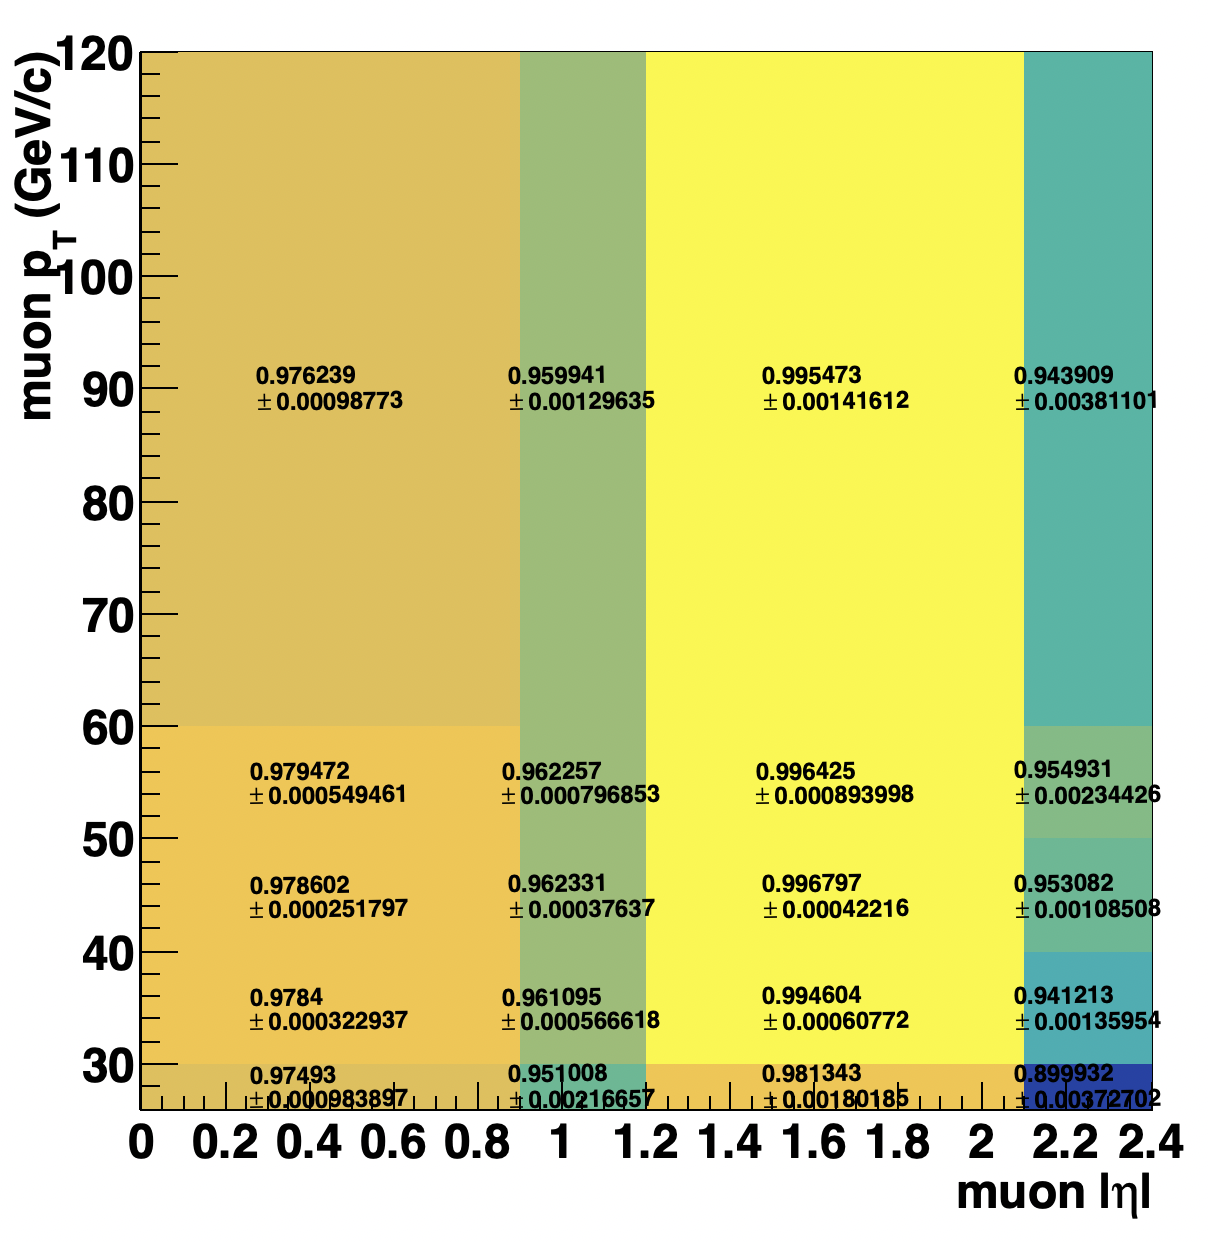
\includegraphics[width=0.45\textwidth]{chapters/Analysis/sectionCalibration/figures/trigger/muTrSF_BCDEF.png}
        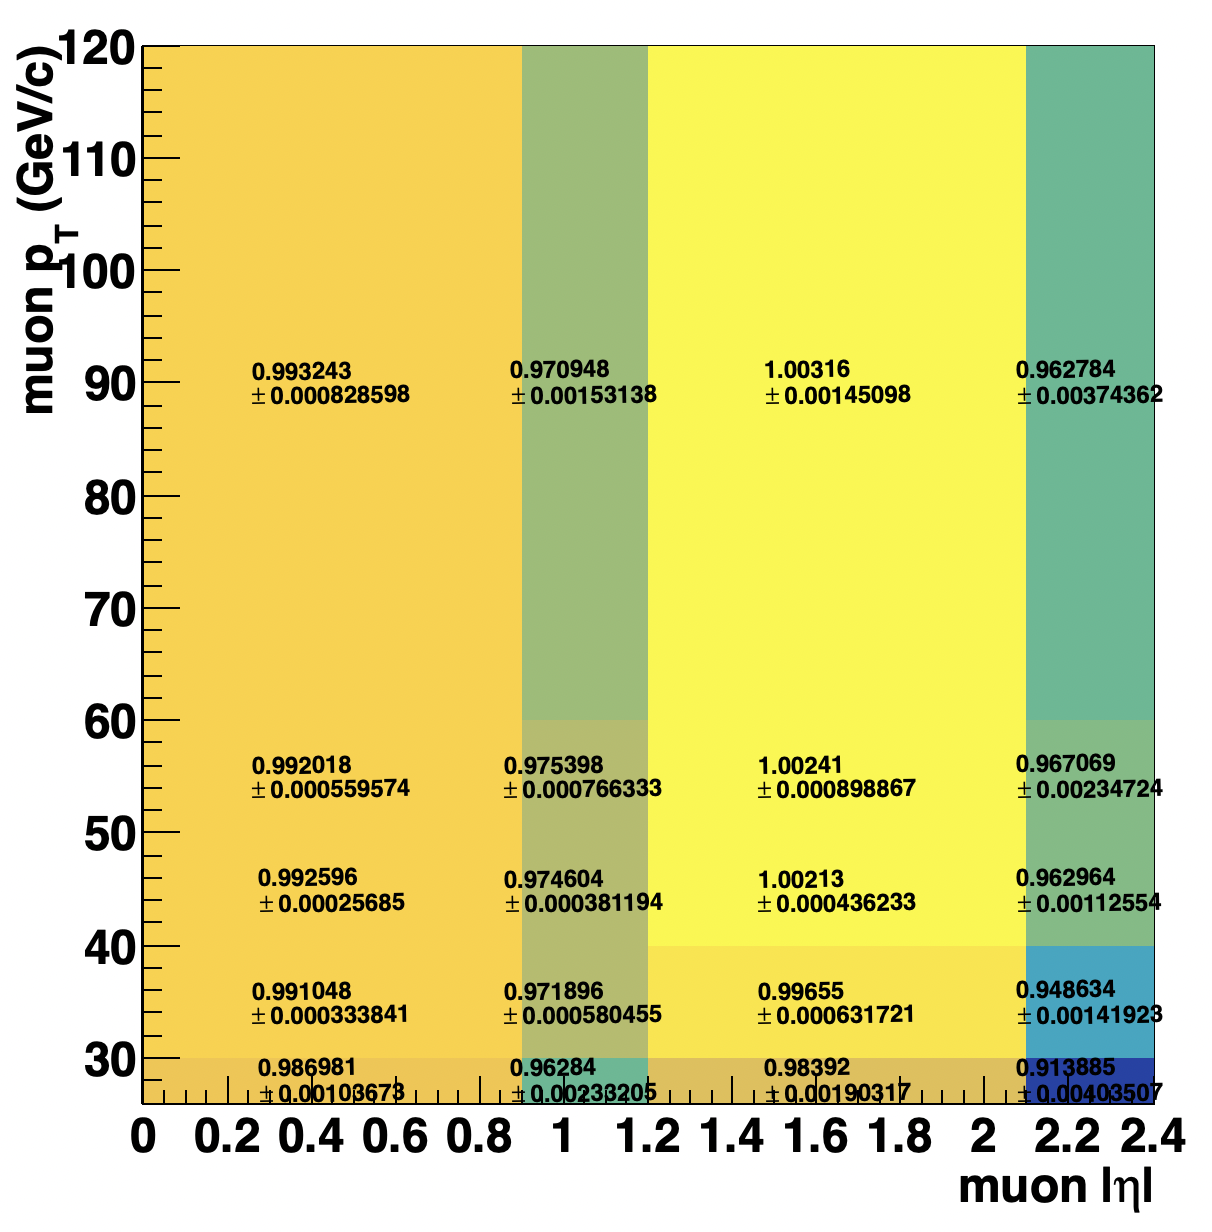
\includegraphics[width=0.45\textwidth]{chapters/Analysis/sectionCalibration/figures/trigger/muTrSF_GH.png}
    \end{block} 
    
    \column{.49\textwidth}
     \begin{block}{electron trigger}
        \centering
        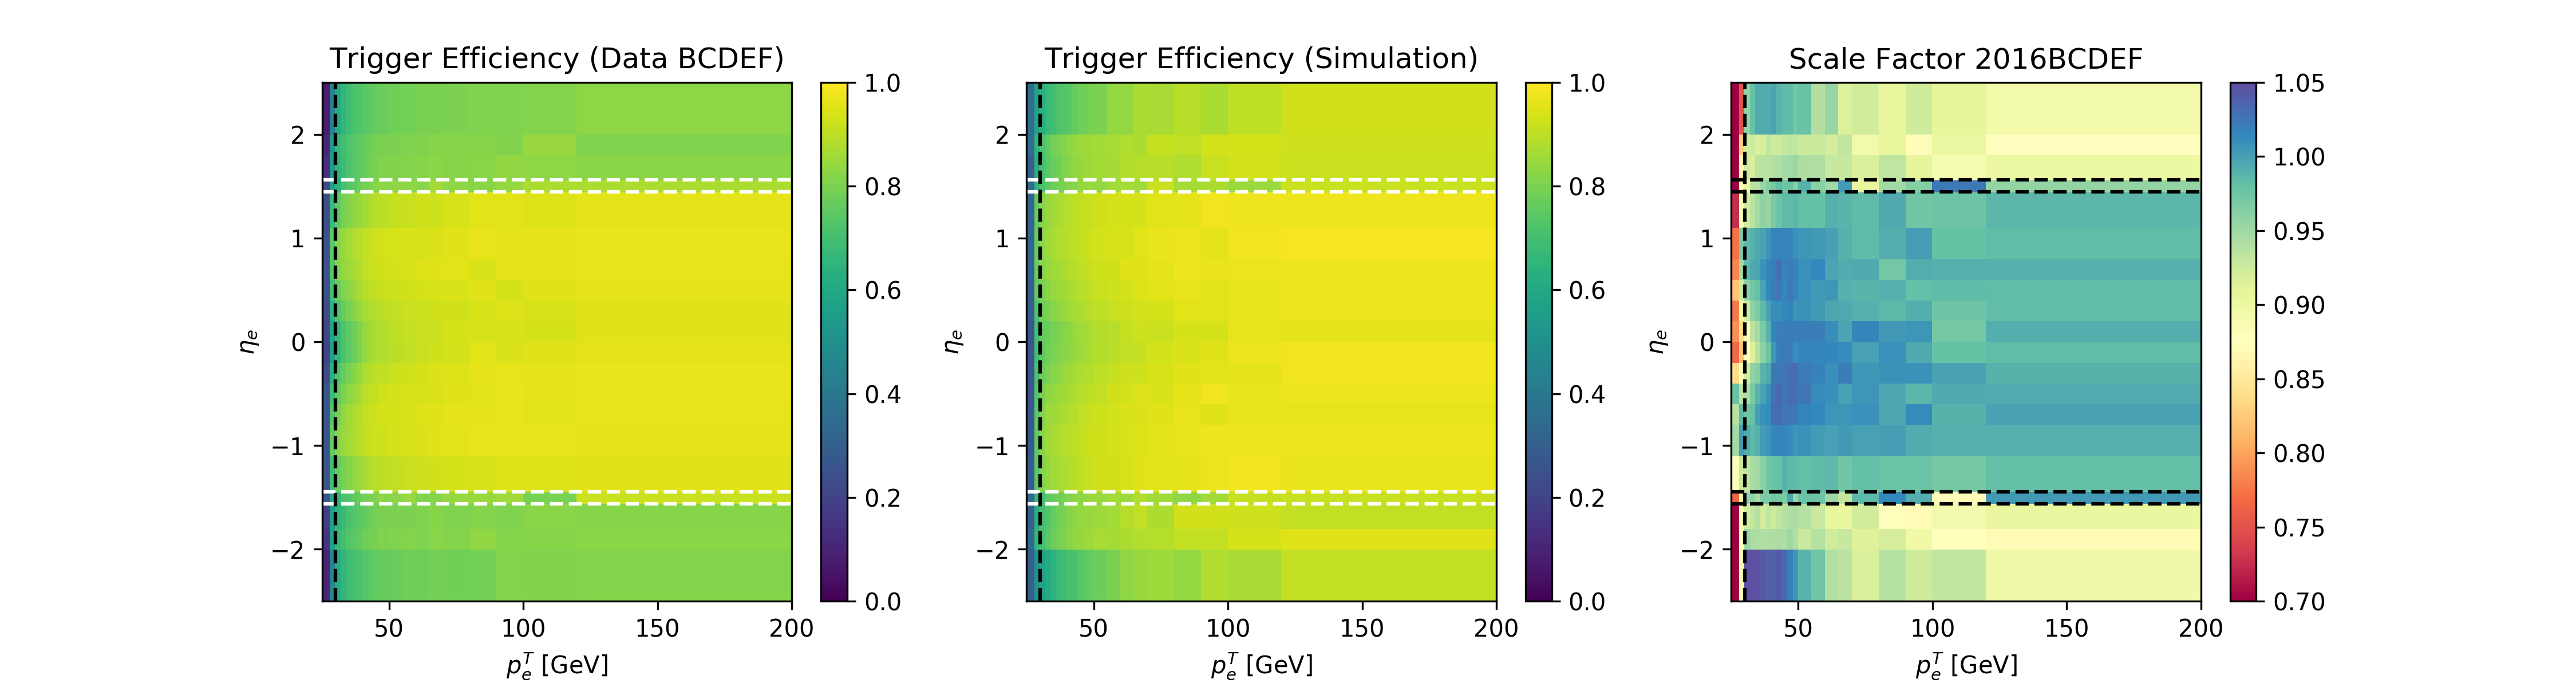
\includegraphics[width=0.45\textwidth, trim=24cm 0 3.7cm 0, clip]{chapters/Analysis/sectionCalibration/figures/eTrigger/eff2d_BCDEF.png}
        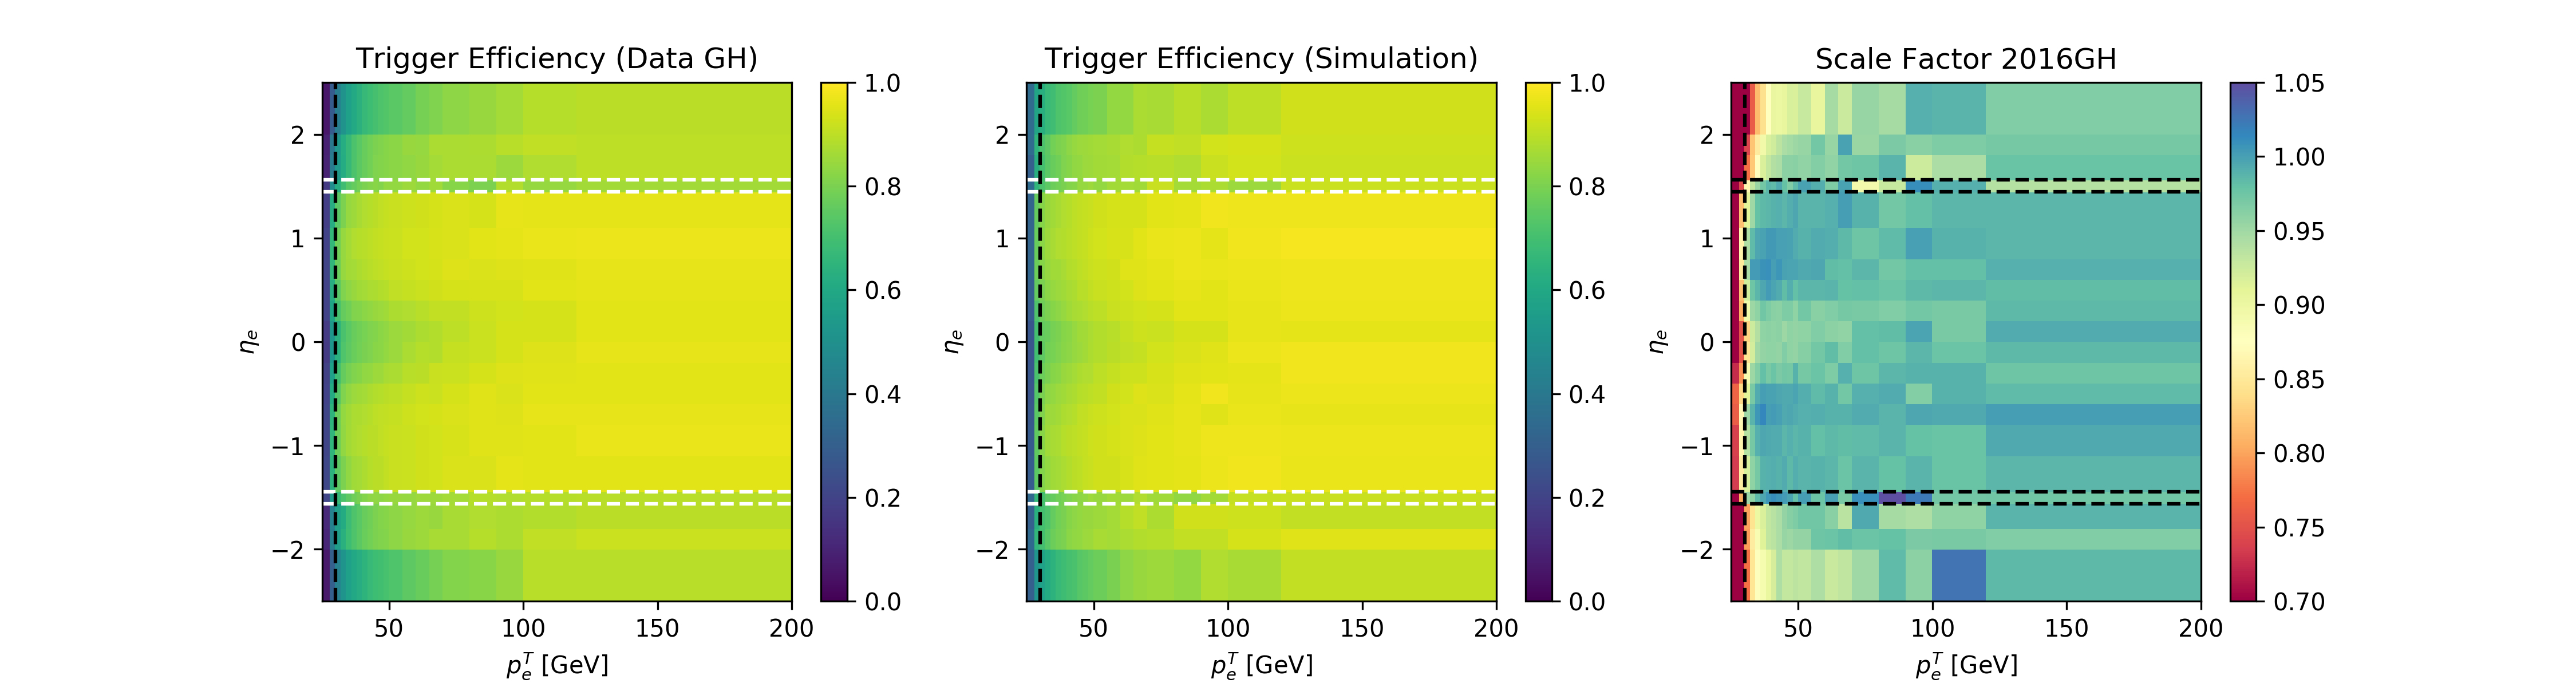
\includegraphics[width=0.45\textwidth, trim=24cm 0 3.7cm 0, clip]{chapters/Analysis/sectionCalibration/figures/eTrigger/eff2d_GH.png}
    \end{block}
    \end{columns}
    
    \begin{block}{electron prefiring correction}
        \begin{columns}
            \column{0.6\textwidth}
            \begin{itemize} 
                \smaller
                \item due to timing issue, L1T signal in higher eta could be treated as from previous bunching crossing by mistake.
                \item the wrong brunching crossing fails the HLT due to absence of the triggering objects, resulting data loss.
                \item this is not simulated. 
                \item corrected by a scale factor calculated from prefirable jets and photons $$ SF = \prod_{i=\PGg,jet}\bigg(1-\epsilon_i(\pt, \eta) \bigg) $$
                \item scale down the events by ~1\%.
            \end{itemize}
            
            \column{0.35\textwidth}
            % 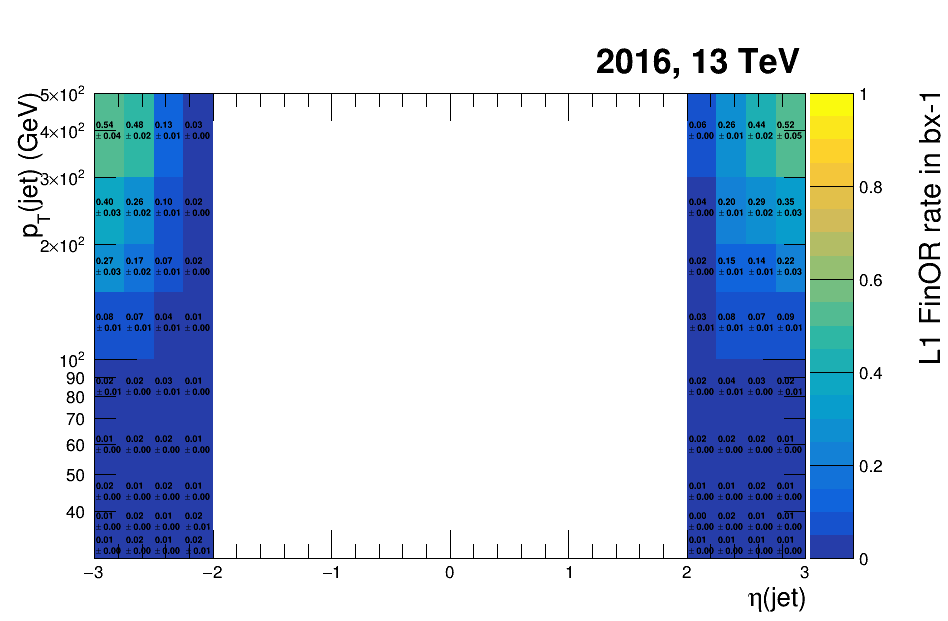
\includegraphics[width=\textwidth]{chapters/Analysis/sectionCalibration/figures/prefiring/L1prefiring_jetpt_2016BtoH.png}
            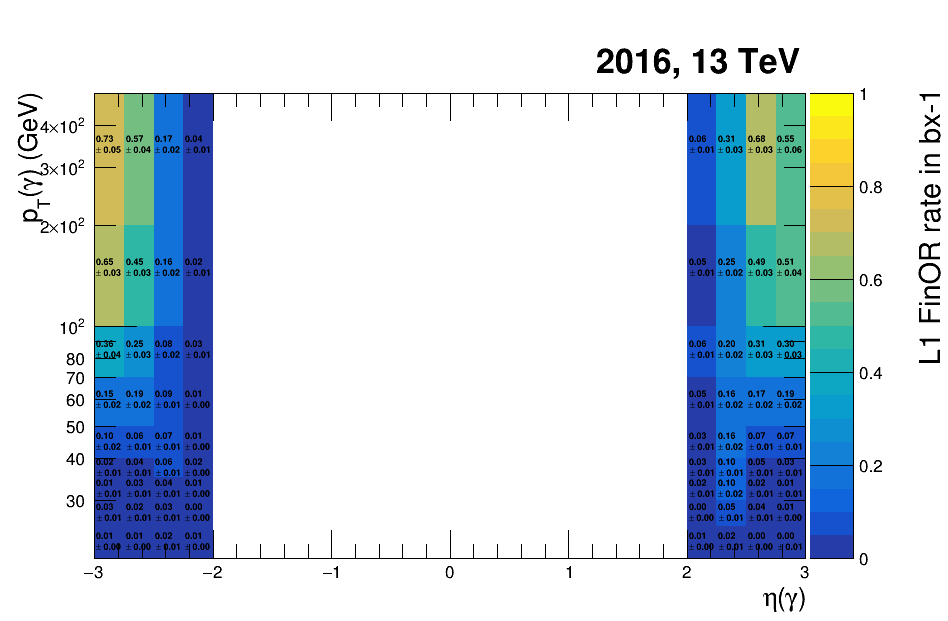
\includegraphics[width=\textwidth]{chapters/Analysis/sectionCalibration/figures/prefiring/L1prefiring_photonpt_2016BtoH.png}
            
        \end{columns}
    \end{block}

\end{frame}


% -------------
% e trigger SF
% -------------
\begin{frame}{uncertainties of e trigger SF}
\smaller
    \begin{columns}
        \column{0.48\textwidth}
        \begin{block}{$SF (\pt, \eta)$ in B-F}
            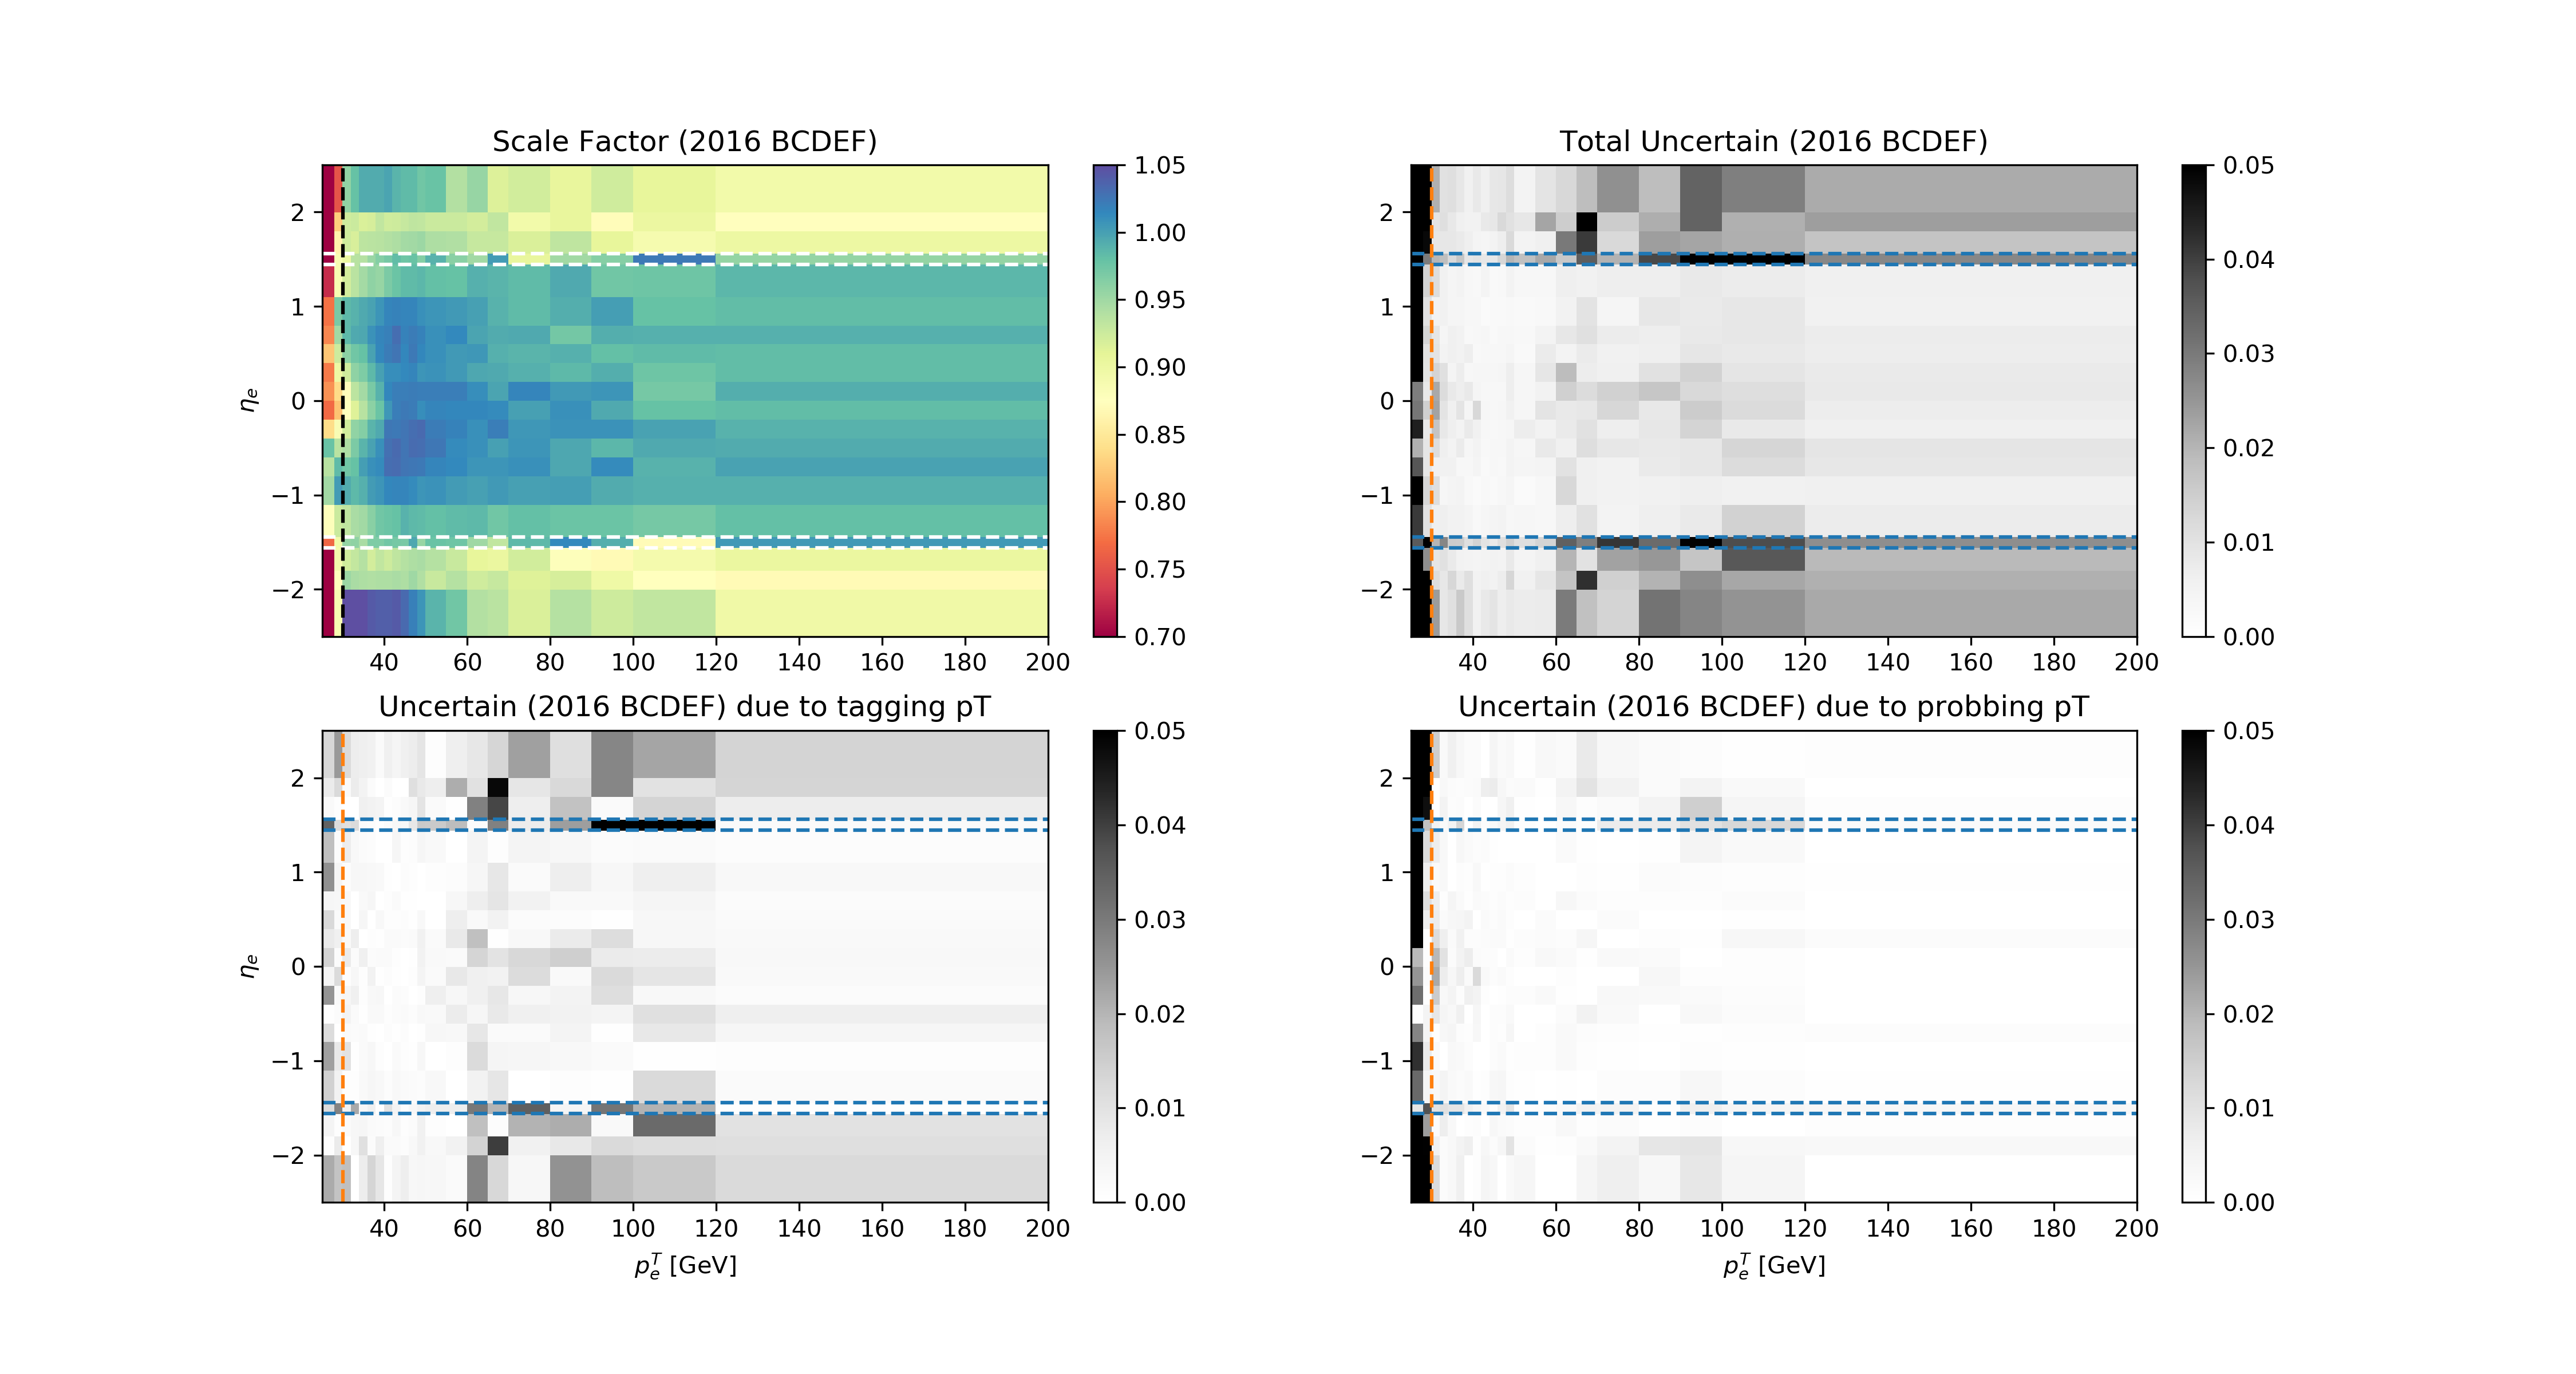
\includegraphics[width=\textwidth,trim=3cm 0 3cm 0, clip]{chapters/Analysis/sectionCalibration/figures/eTrigger/result_BCDEF.png}
        \end{block}
        
        \column{0.48\textwidth}
        \begin{block}{$SF (\pt, \eta)$ in GH}
            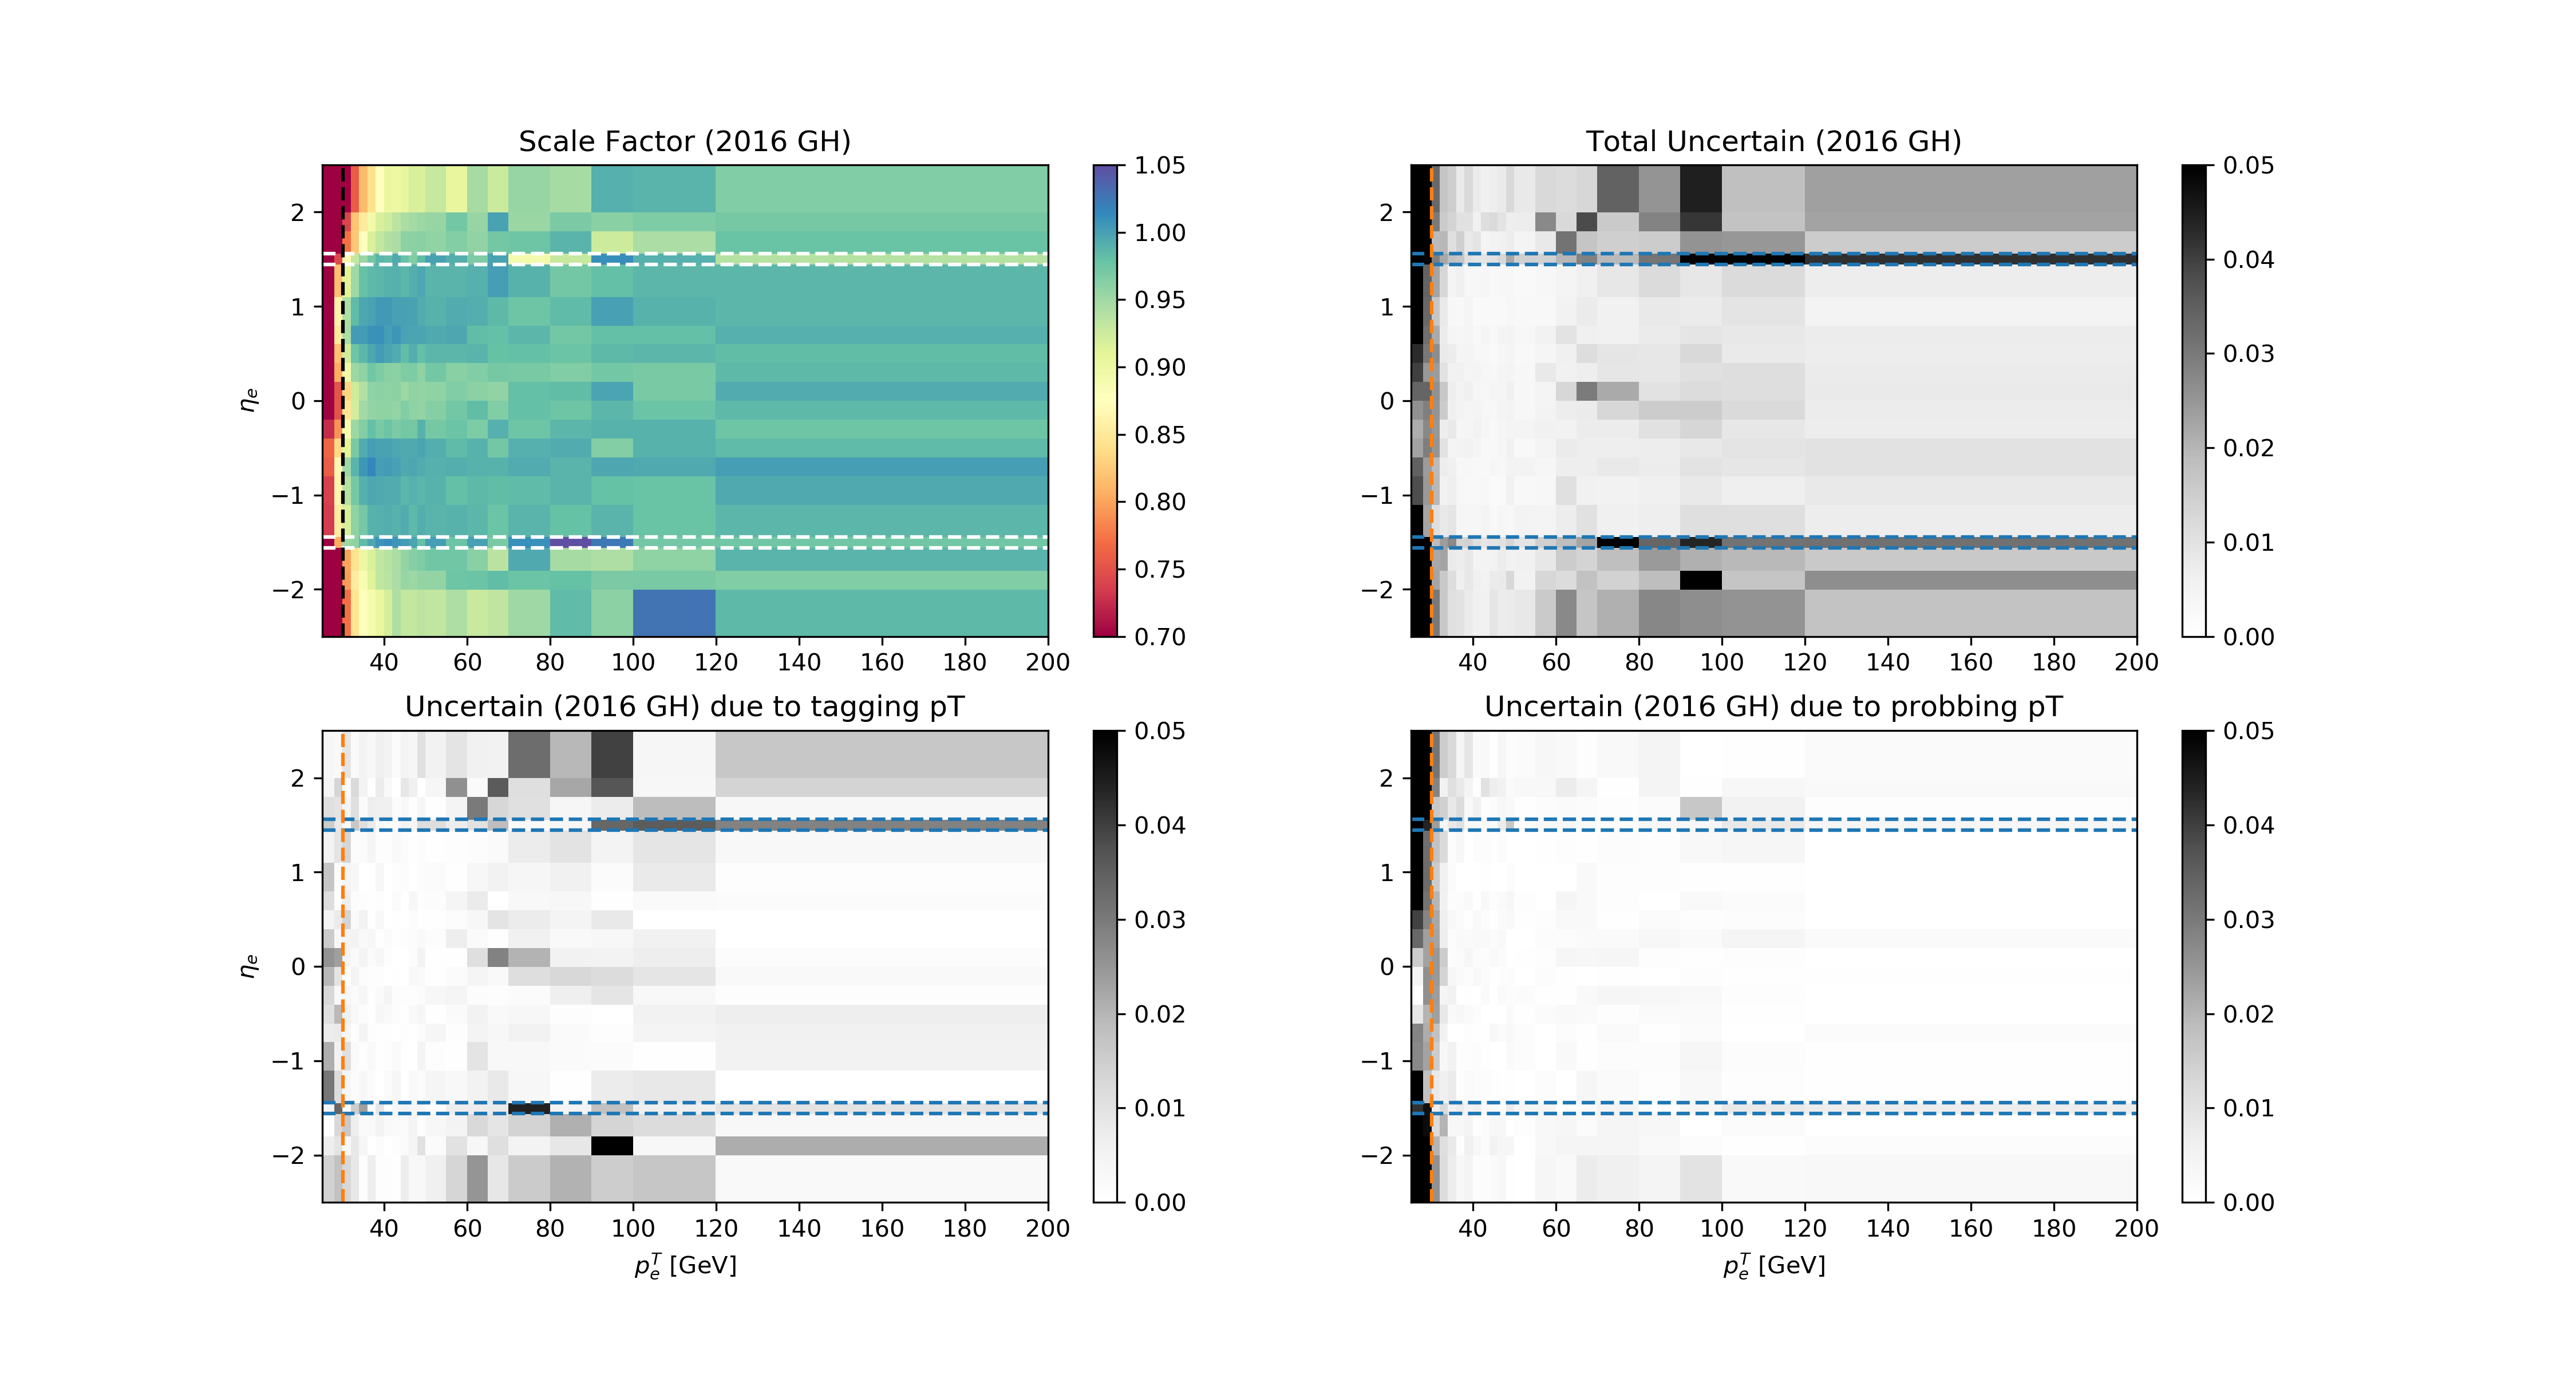
\includegraphics[width=\textwidth,trim=3cm 0 3cm 0, clip]{chapters/Analysis/sectionCalibration/figures/eTrigger/result_GH.png}
        \end{block}
    \end{columns}

    \vspace{0.05\textheight}
    \begin{itemize}
        \item Split $SF (\pt, \eta)$ measurement into BCDEF and GH periods. (due to a problem with the readout pre-amplifiers of Si-strip fixed before G.)
                    
        \item The systematic uncertainty of the $SF (\pt, \eta)$ is estimated by ``two shifts"
        \begin{itemize}
        \smaller
            \item shift up the \pt threshold for tagging electron by 10\GeV to simulate a different trigger. This estimates the systematical effect that some L1 seed could have a threshold of 32\GeV.
            \item shift up and down the probing electron \pt by 0.5\GeV. This estimates the effect of the electron energy scale.
        \end{itemize}
    \end{itemize}
\end{frame}








% -------------
% j->tau fakes
% -------------


\begin{frame}{$j\to \PGth$ Fakes}
\smaller
    \begin{columns}
        \column{0.32\textwidth}
        \begin{block}{$\cmm + \PGth$}
            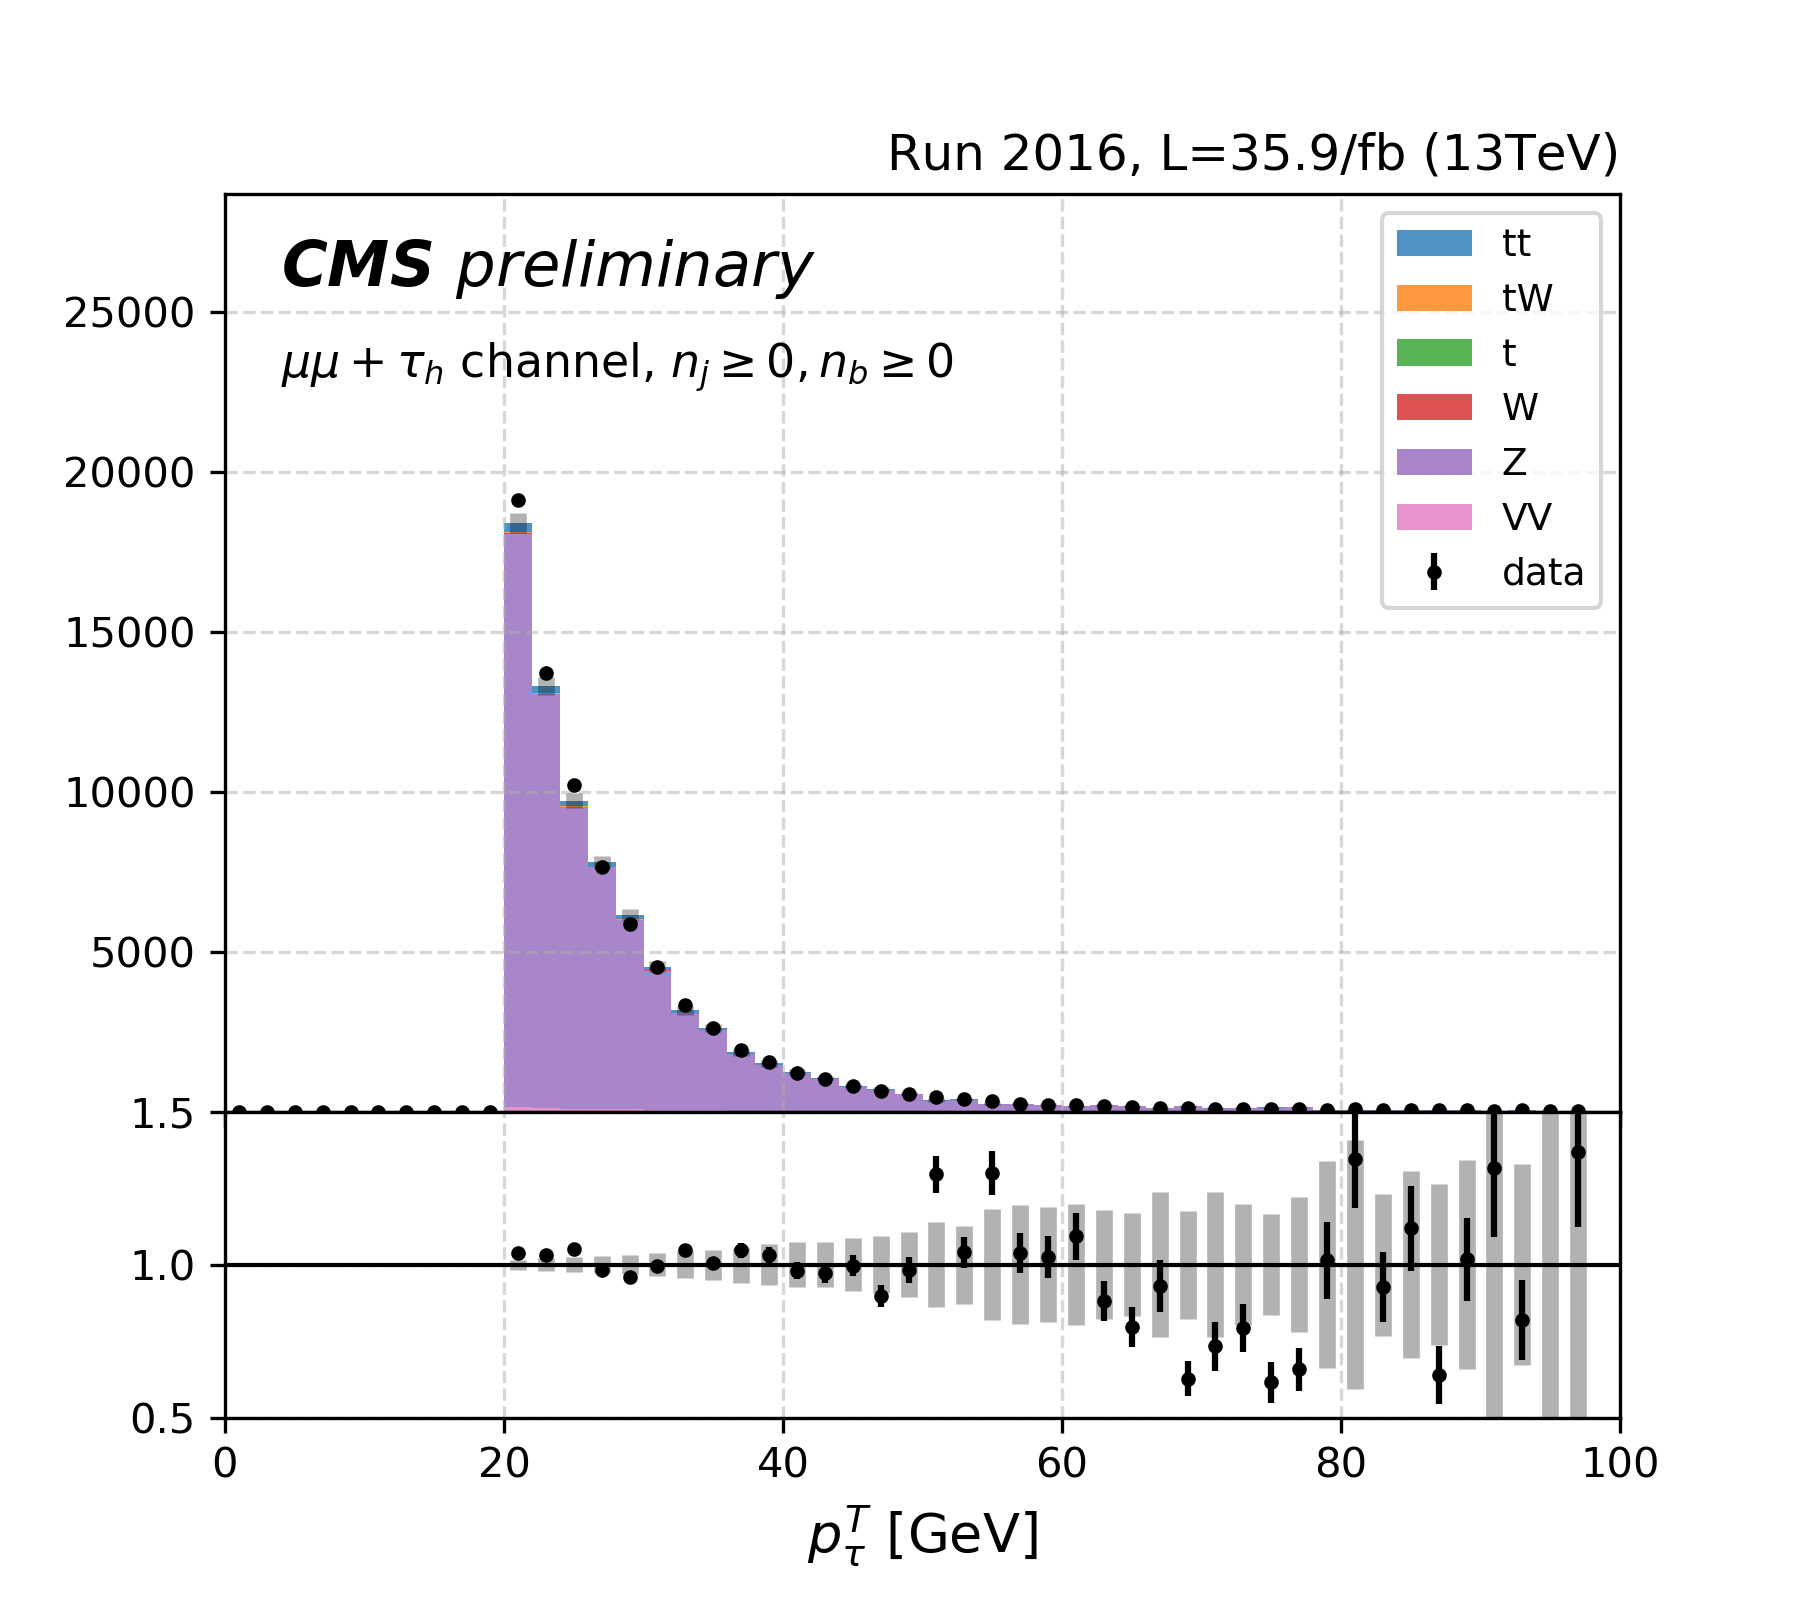
\includegraphics[width=\textwidth]{chapters/Analysis/sectionCalibration/figures/jetToTauh/mumutau_tauPt_pickles_lltauTight.png}
            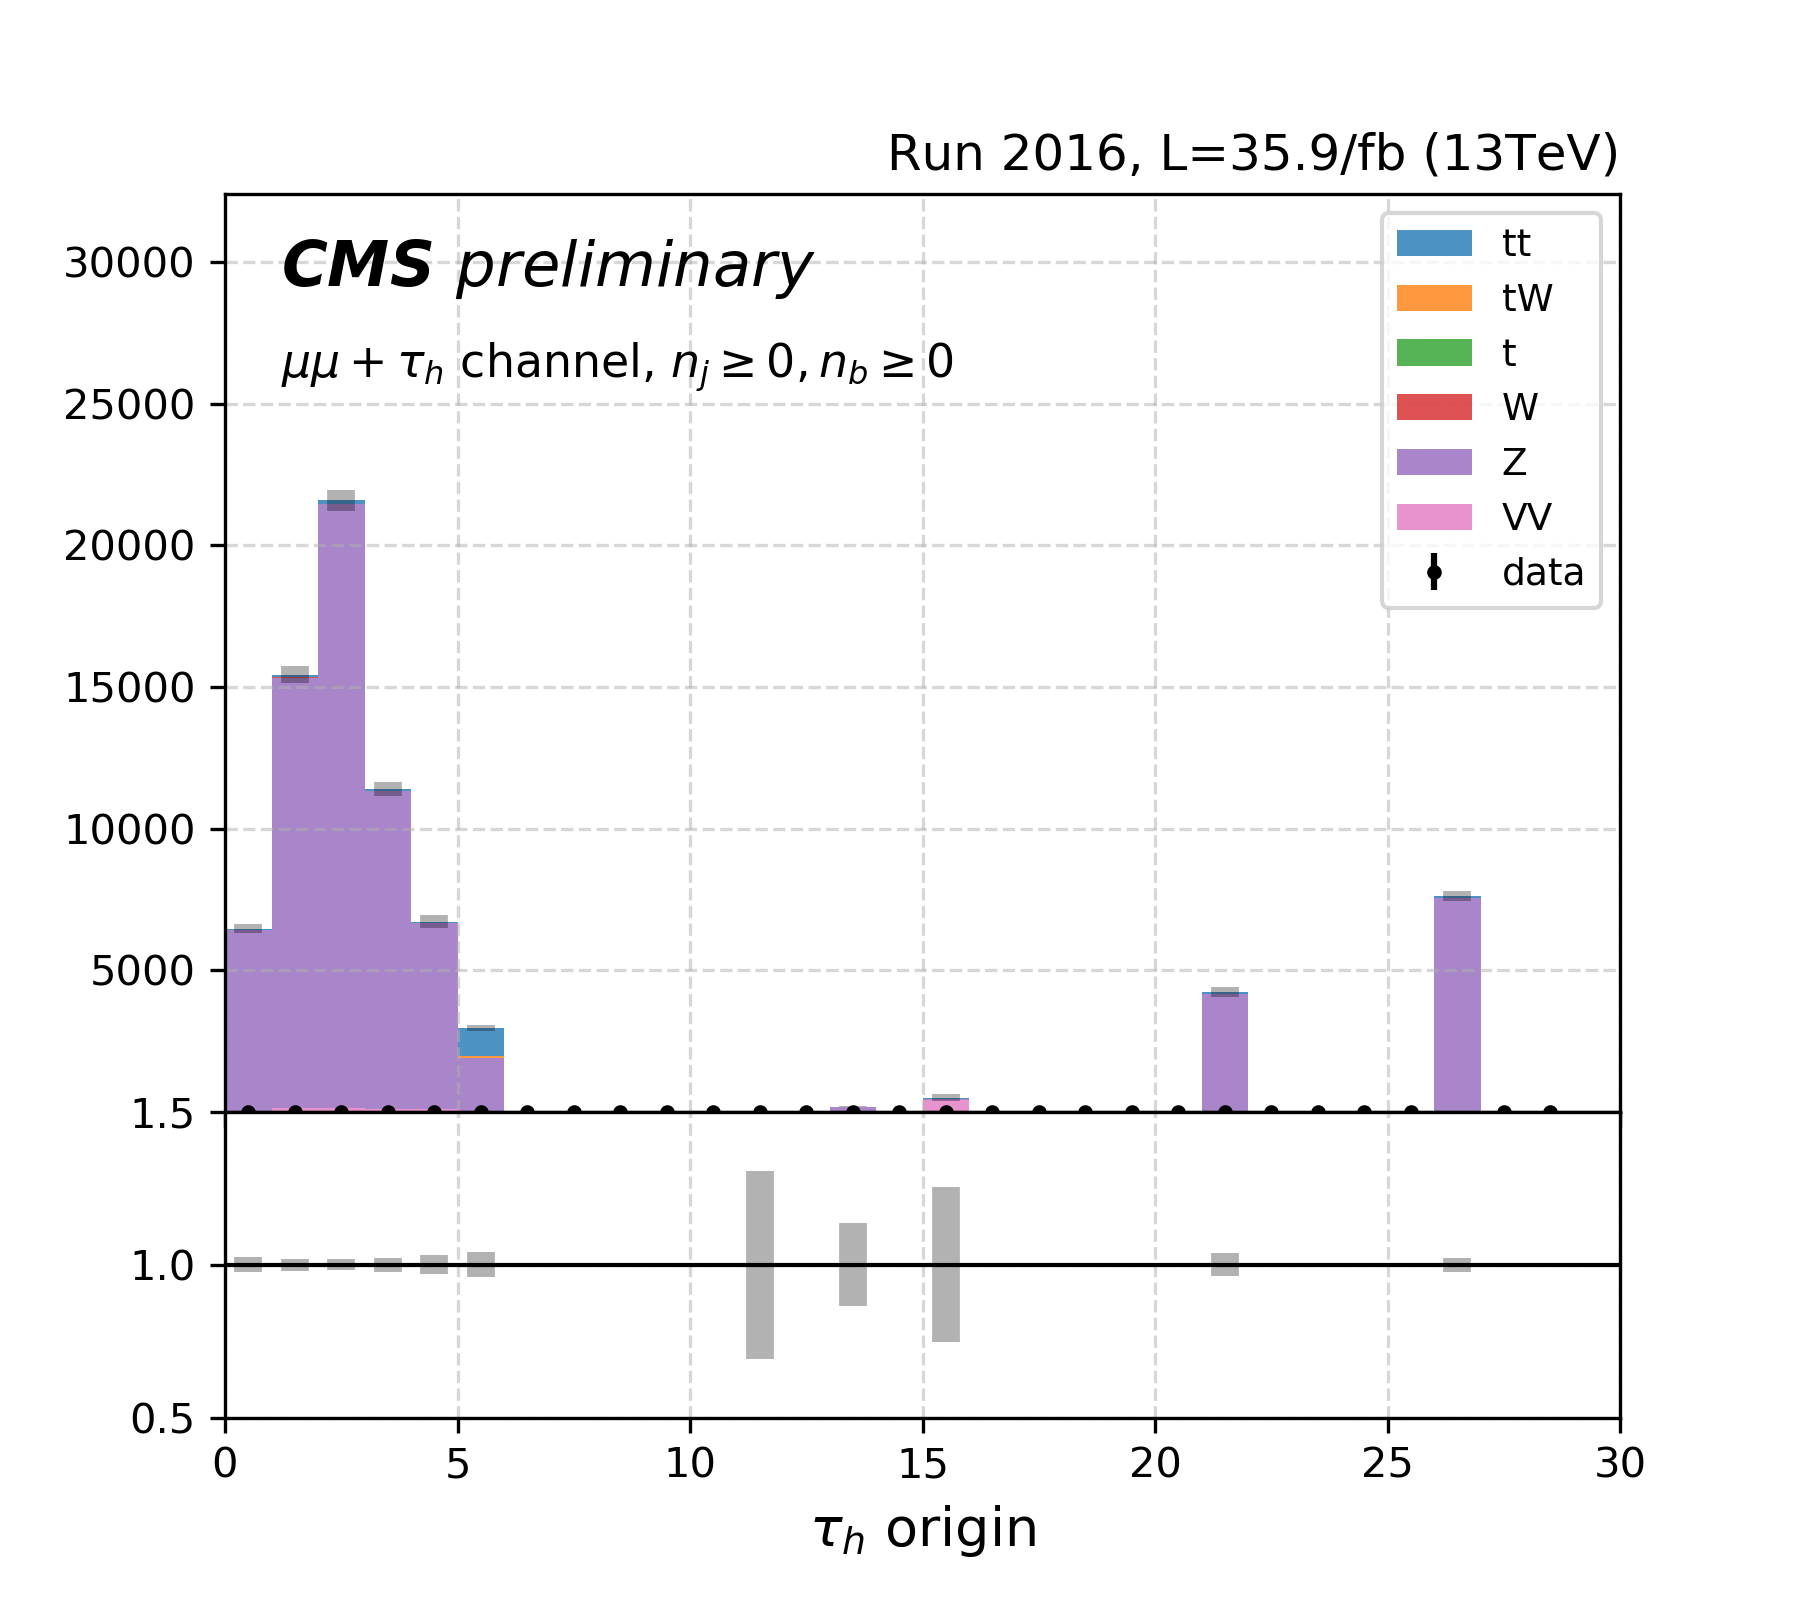
\includegraphics[width=\textwidth]{chapters/Analysis/sectionCalibration/figures/jetToTauh/mumutau_tauGenFlavor_pickles_lltauTight.png}
        \end{block}
        
        \column{0.32\textwidth}
        \begin{block}{$\cee + \PGth$}
            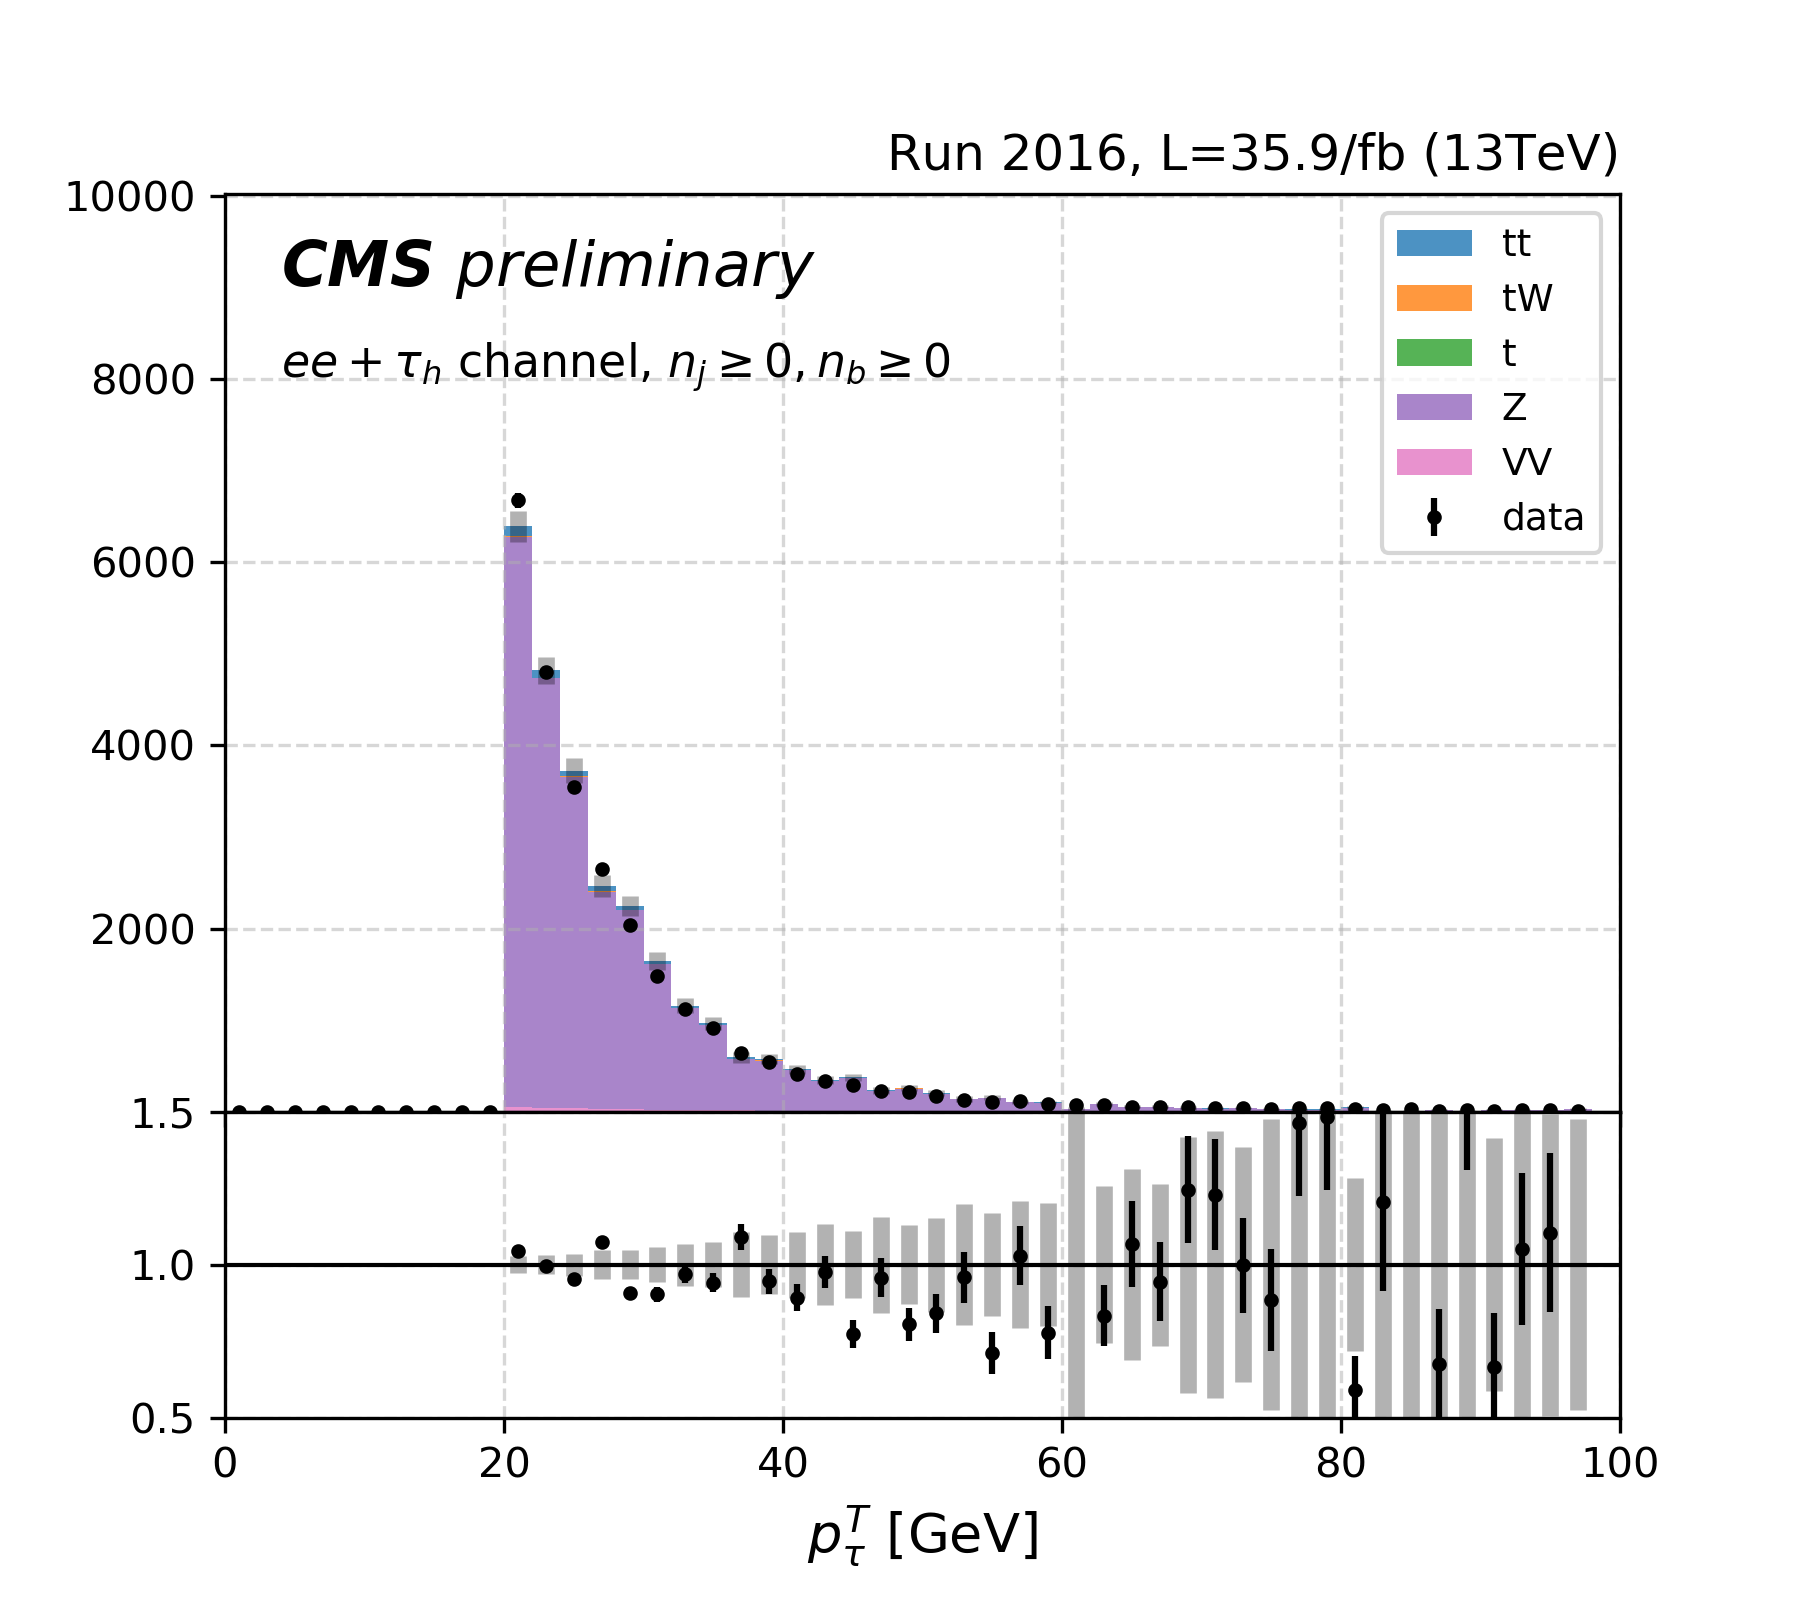
\includegraphics[width=\textwidth]{chapters/Analysis/sectionCalibration/figures/jetToTauh/eetau_tauPt_pickles_lltauTight.png}
            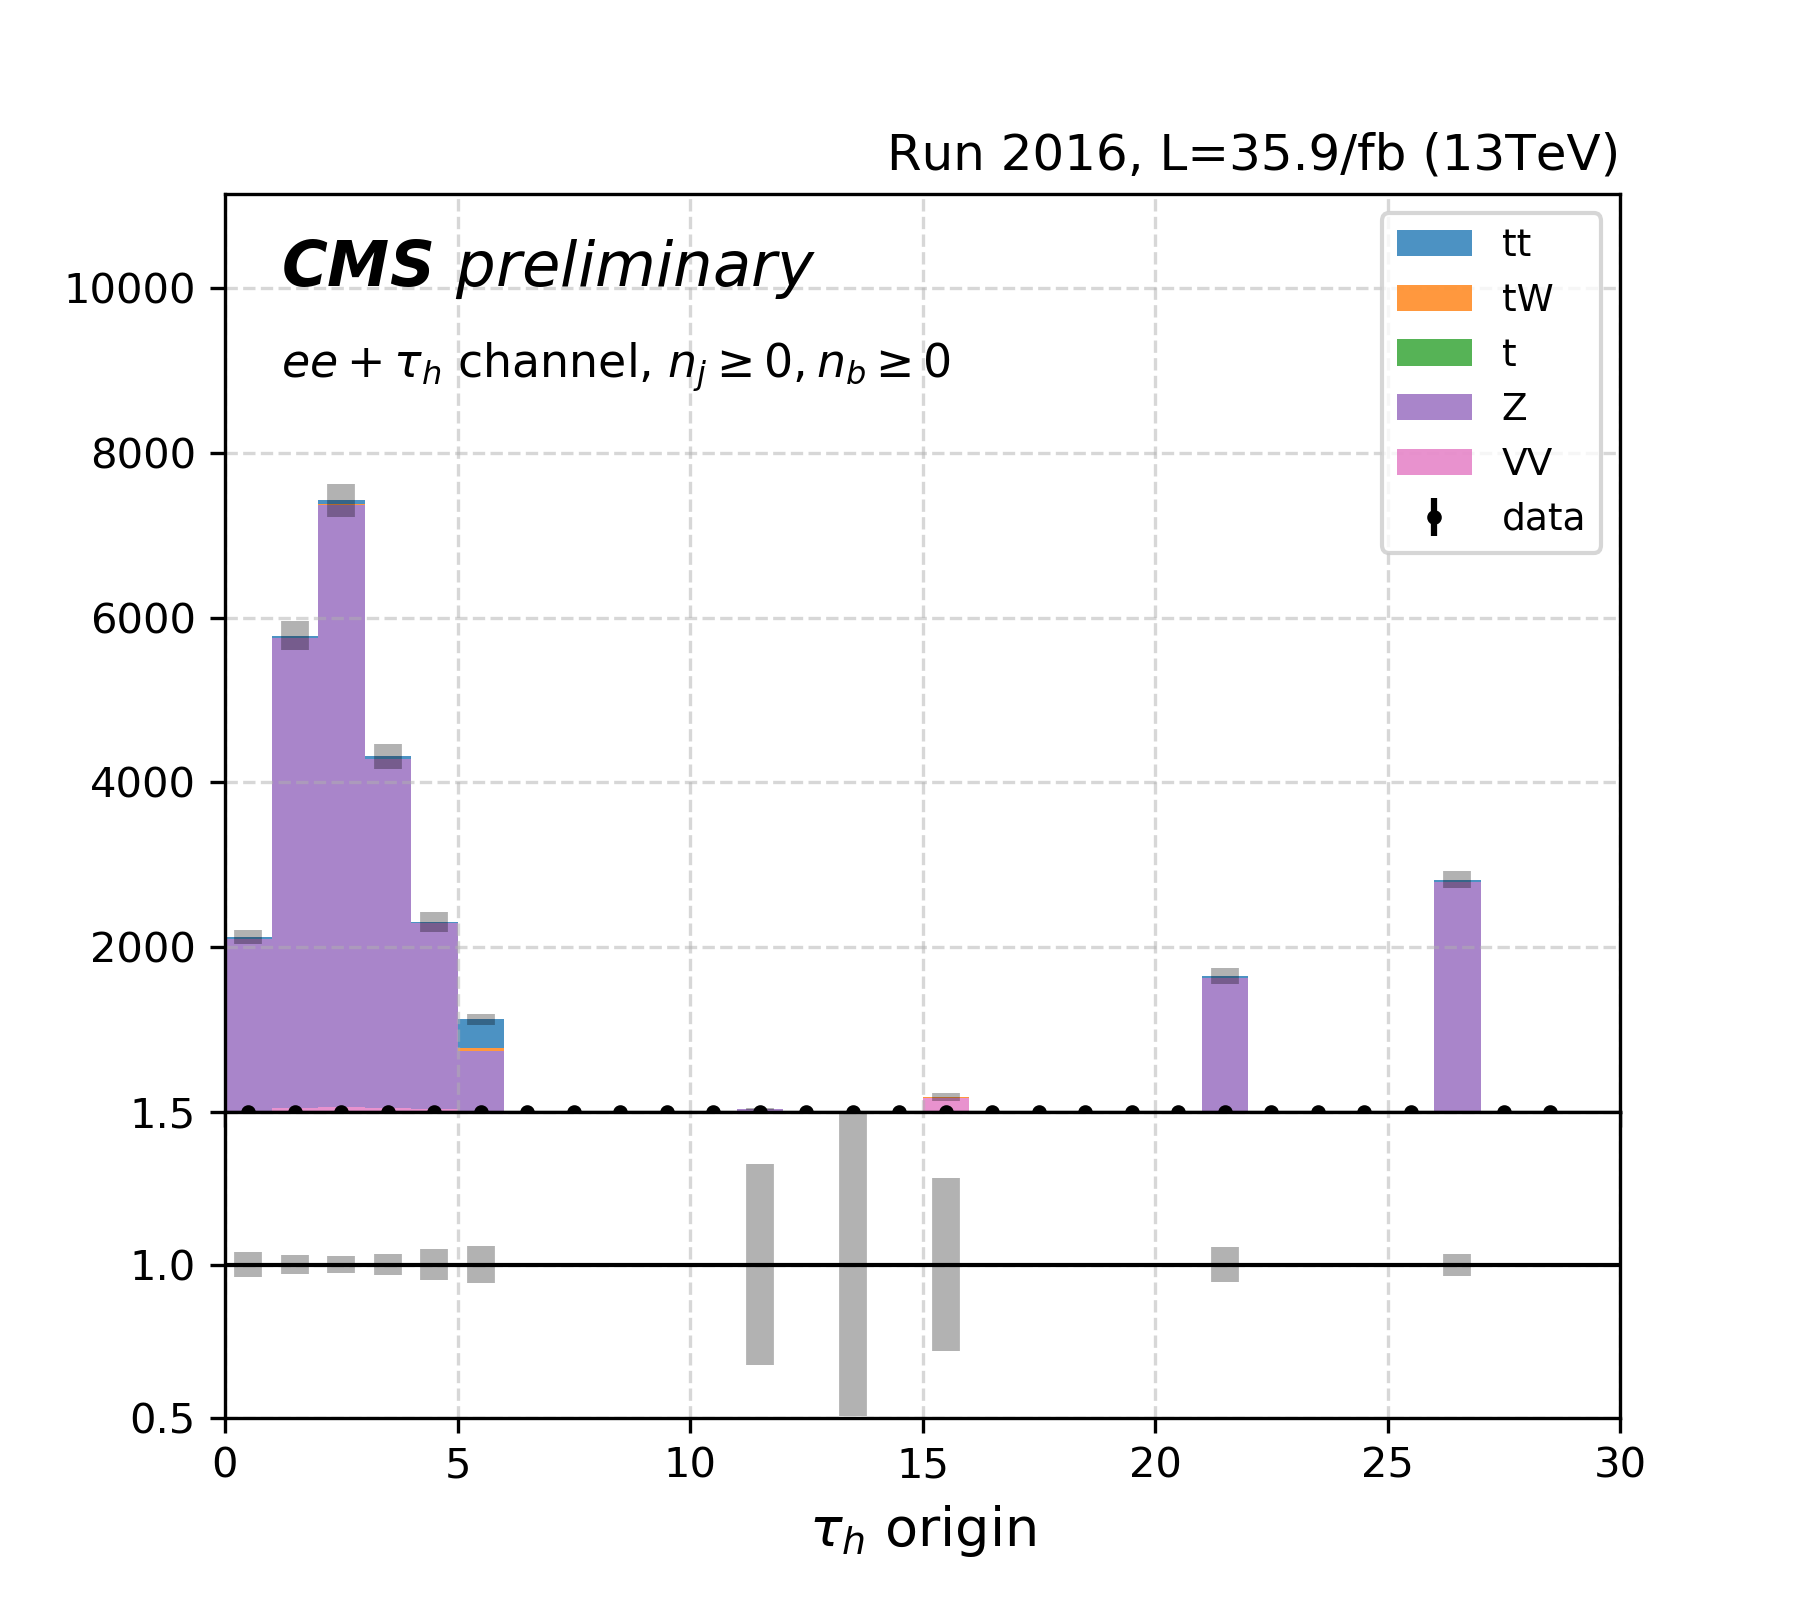
\includegraphics[width=\textwidth]{chapters/Analysis/sectionCalibration/figures/jetToTauh/eetau_tauGenFlavor_pickles_lltauTight.png}
        \end{block}
    
        \column{0.32\textwidth}
        \begin{block}{$\cem + \PGth$}
        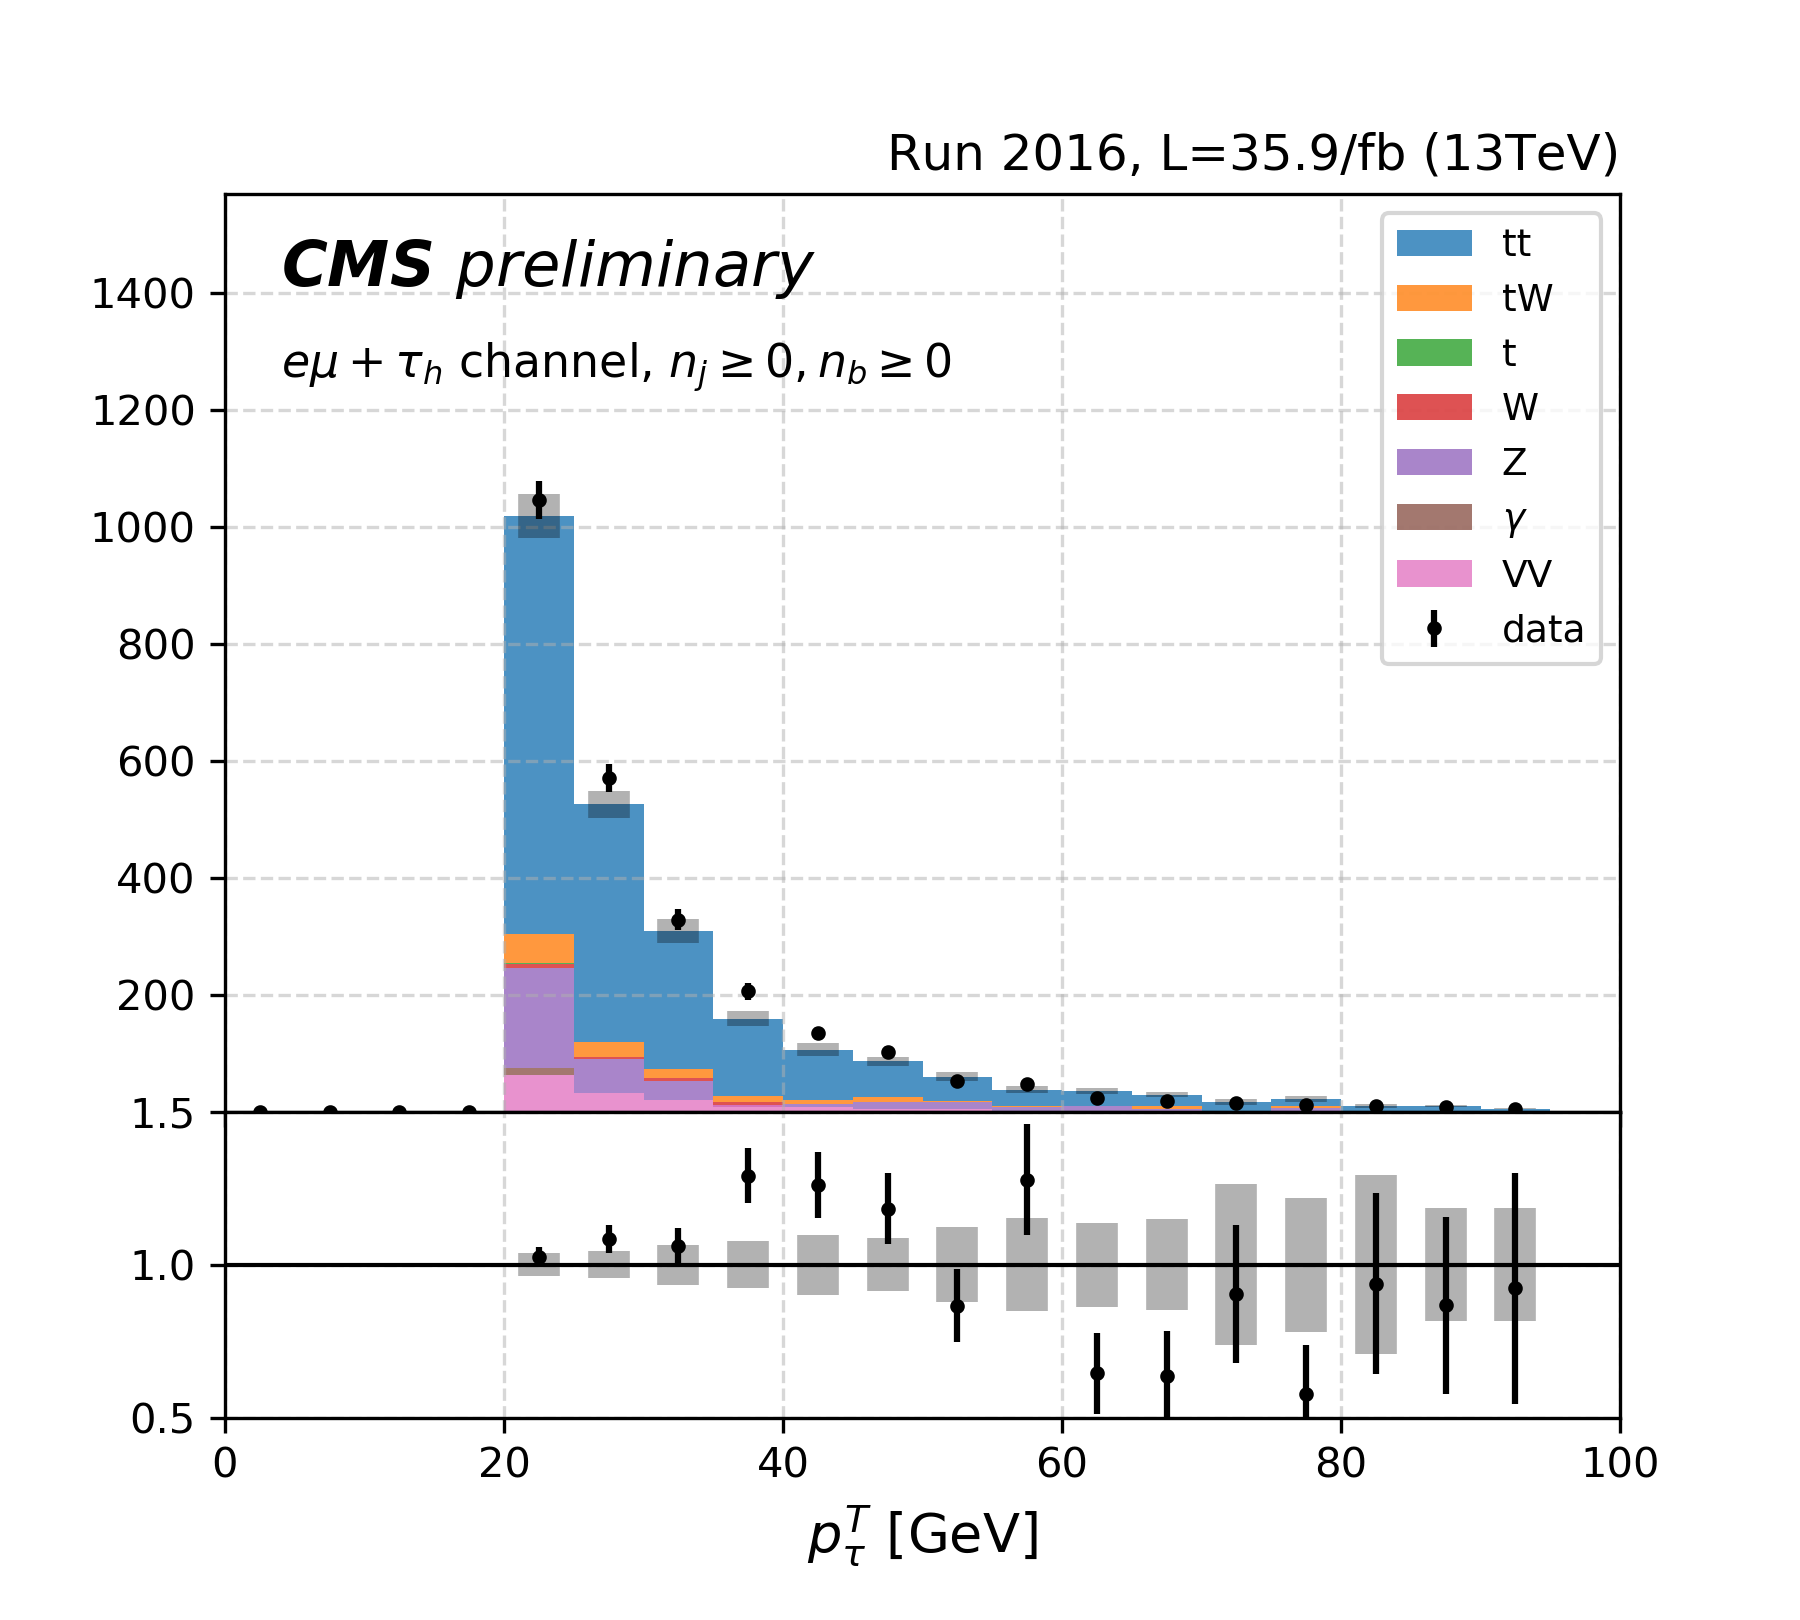
\includegraphics[width=\textwidth]{chapters/Analysis/sectionCalibration/figures/jetToTauh/emutau_tauPt_pickles_lltauTight.png}
        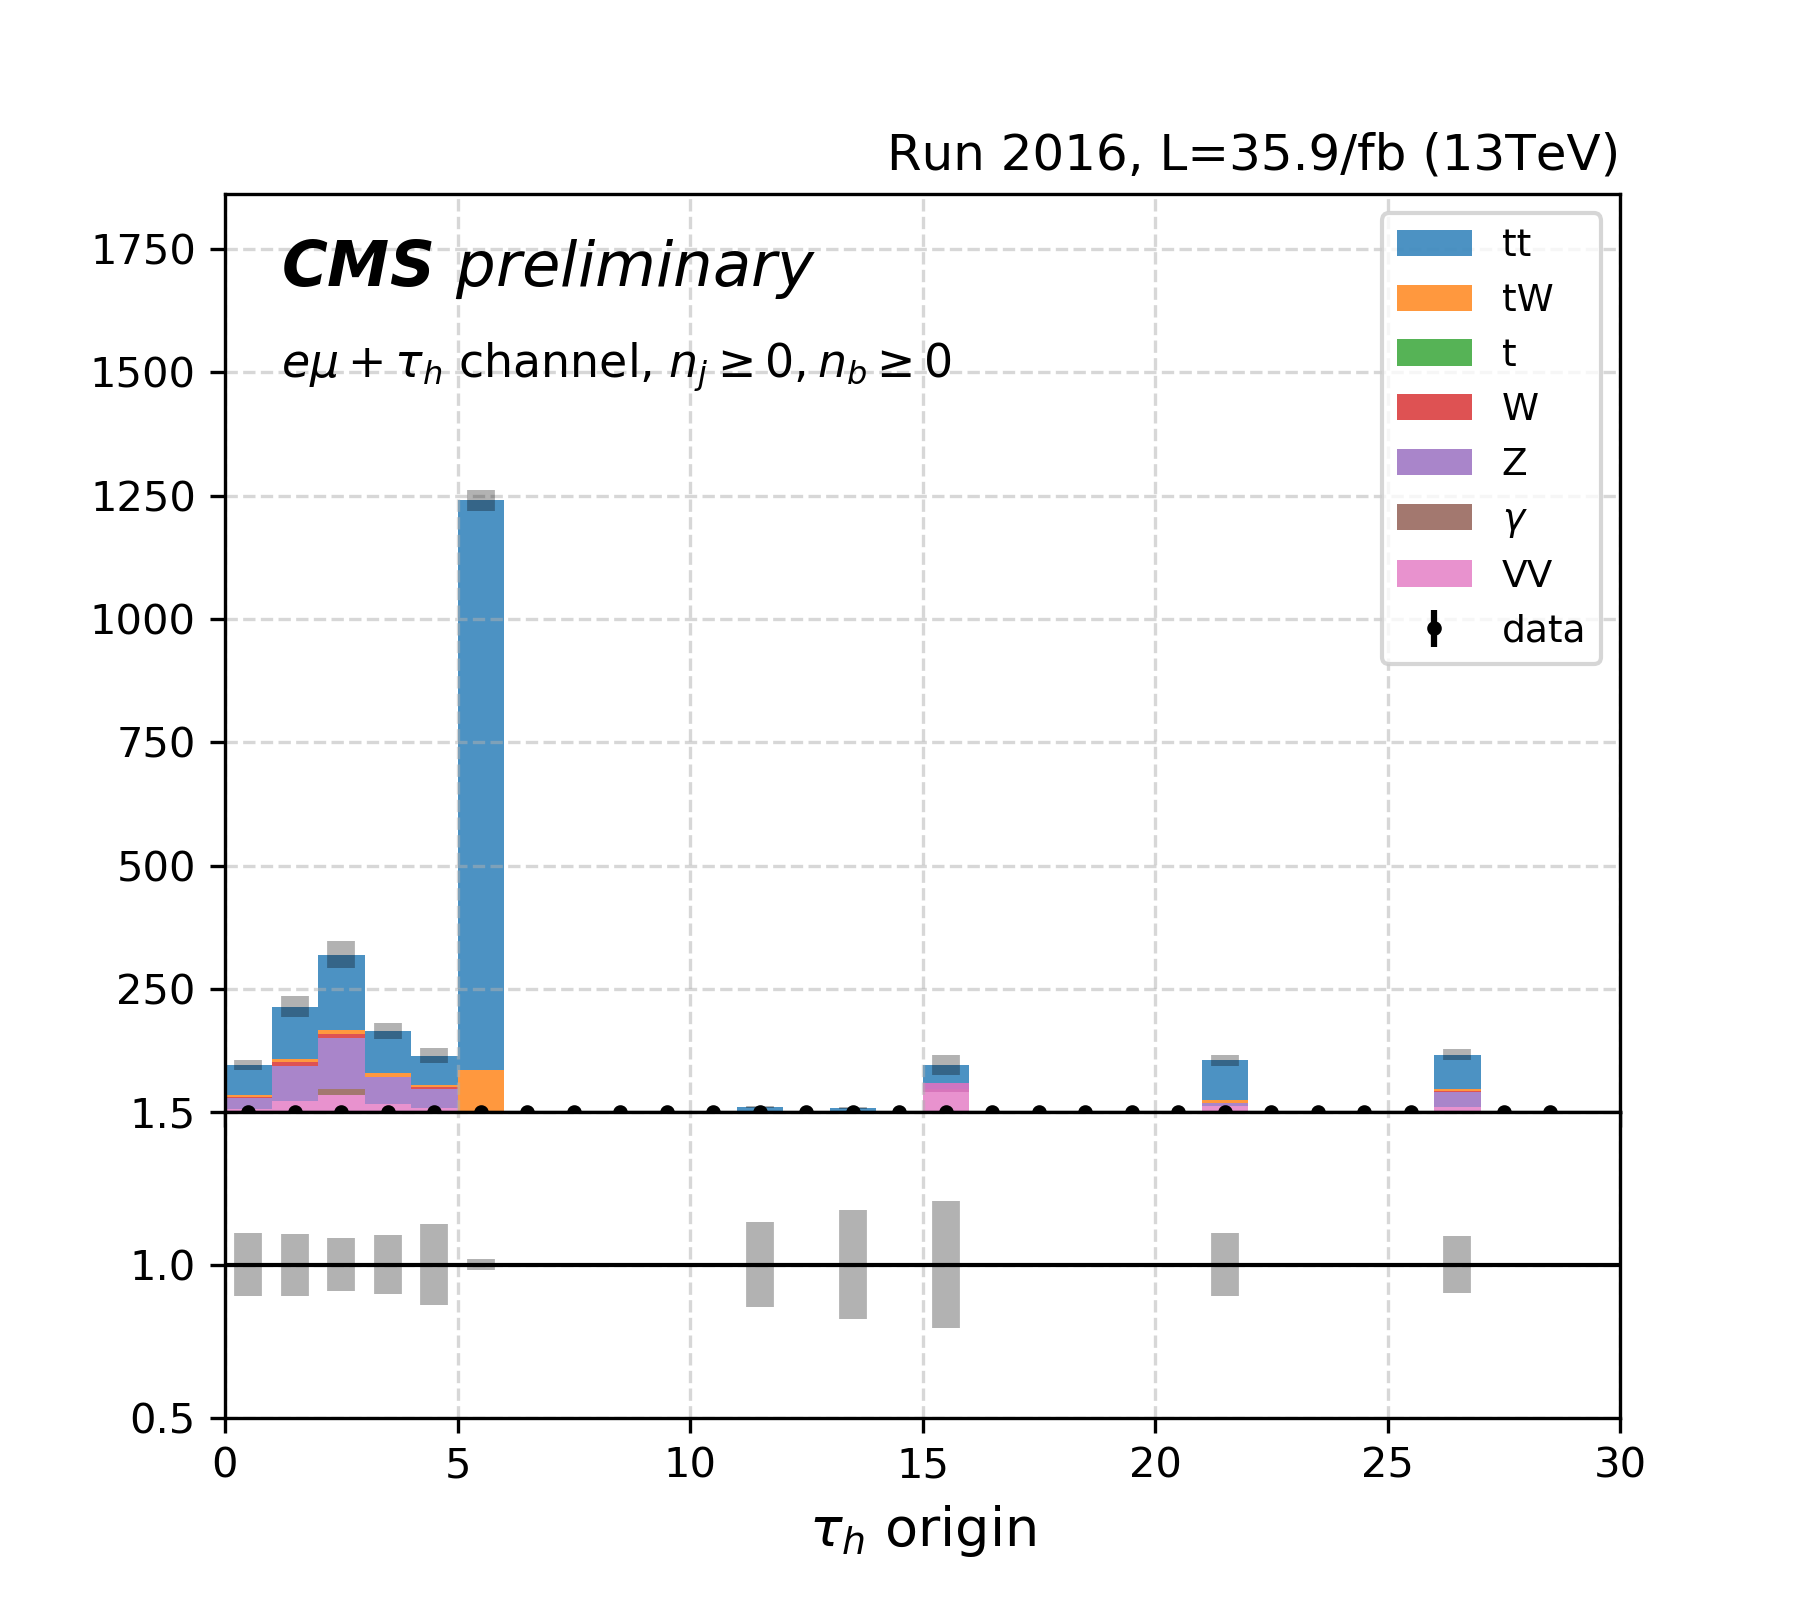
\includegraphics[width=\textwidth]{chapters/Analysis/sectionCalibration/figures/jetToTauh/emutau_tauGenFlavor_pickles_lltauTight.png}
        \end{block}
        
    \end{columns}

\end{frame}


\begin{frame}{}
\smaller
    \begin{block}{$SF_{j\to \PGth}(\pt)$}
    \centering
    Tight \hspace{0.45\textwidth} VTight \\
    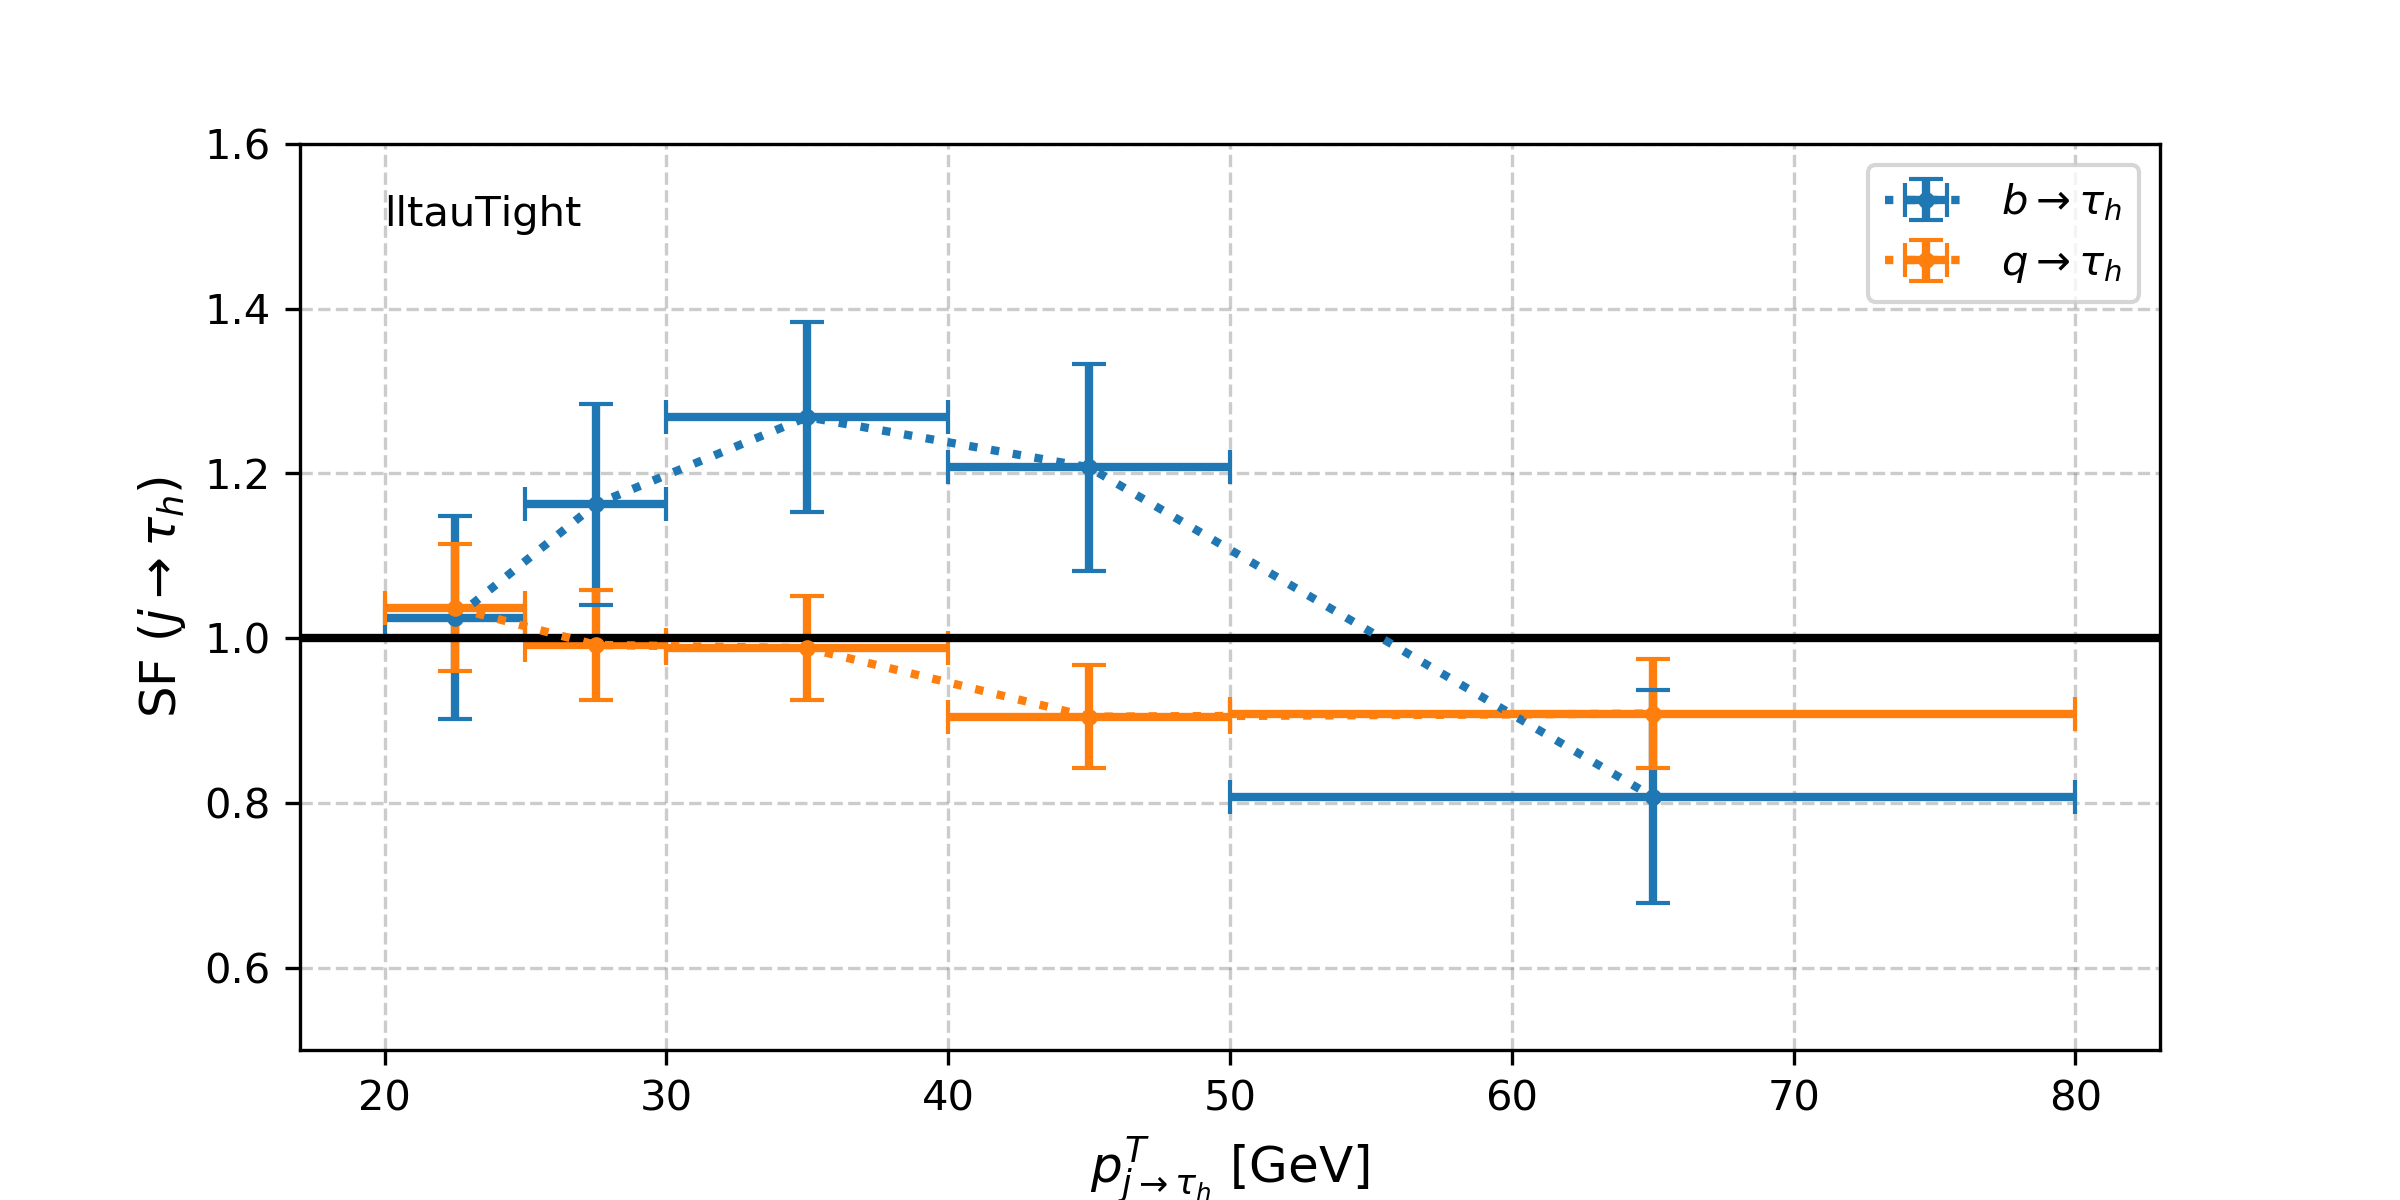
\includegraphics[width=0.49\textwidth]{chapters/Analysis/sectionCalibration/figures/jetToTauh/fit2_ptflavor2_lltauTight.png}
    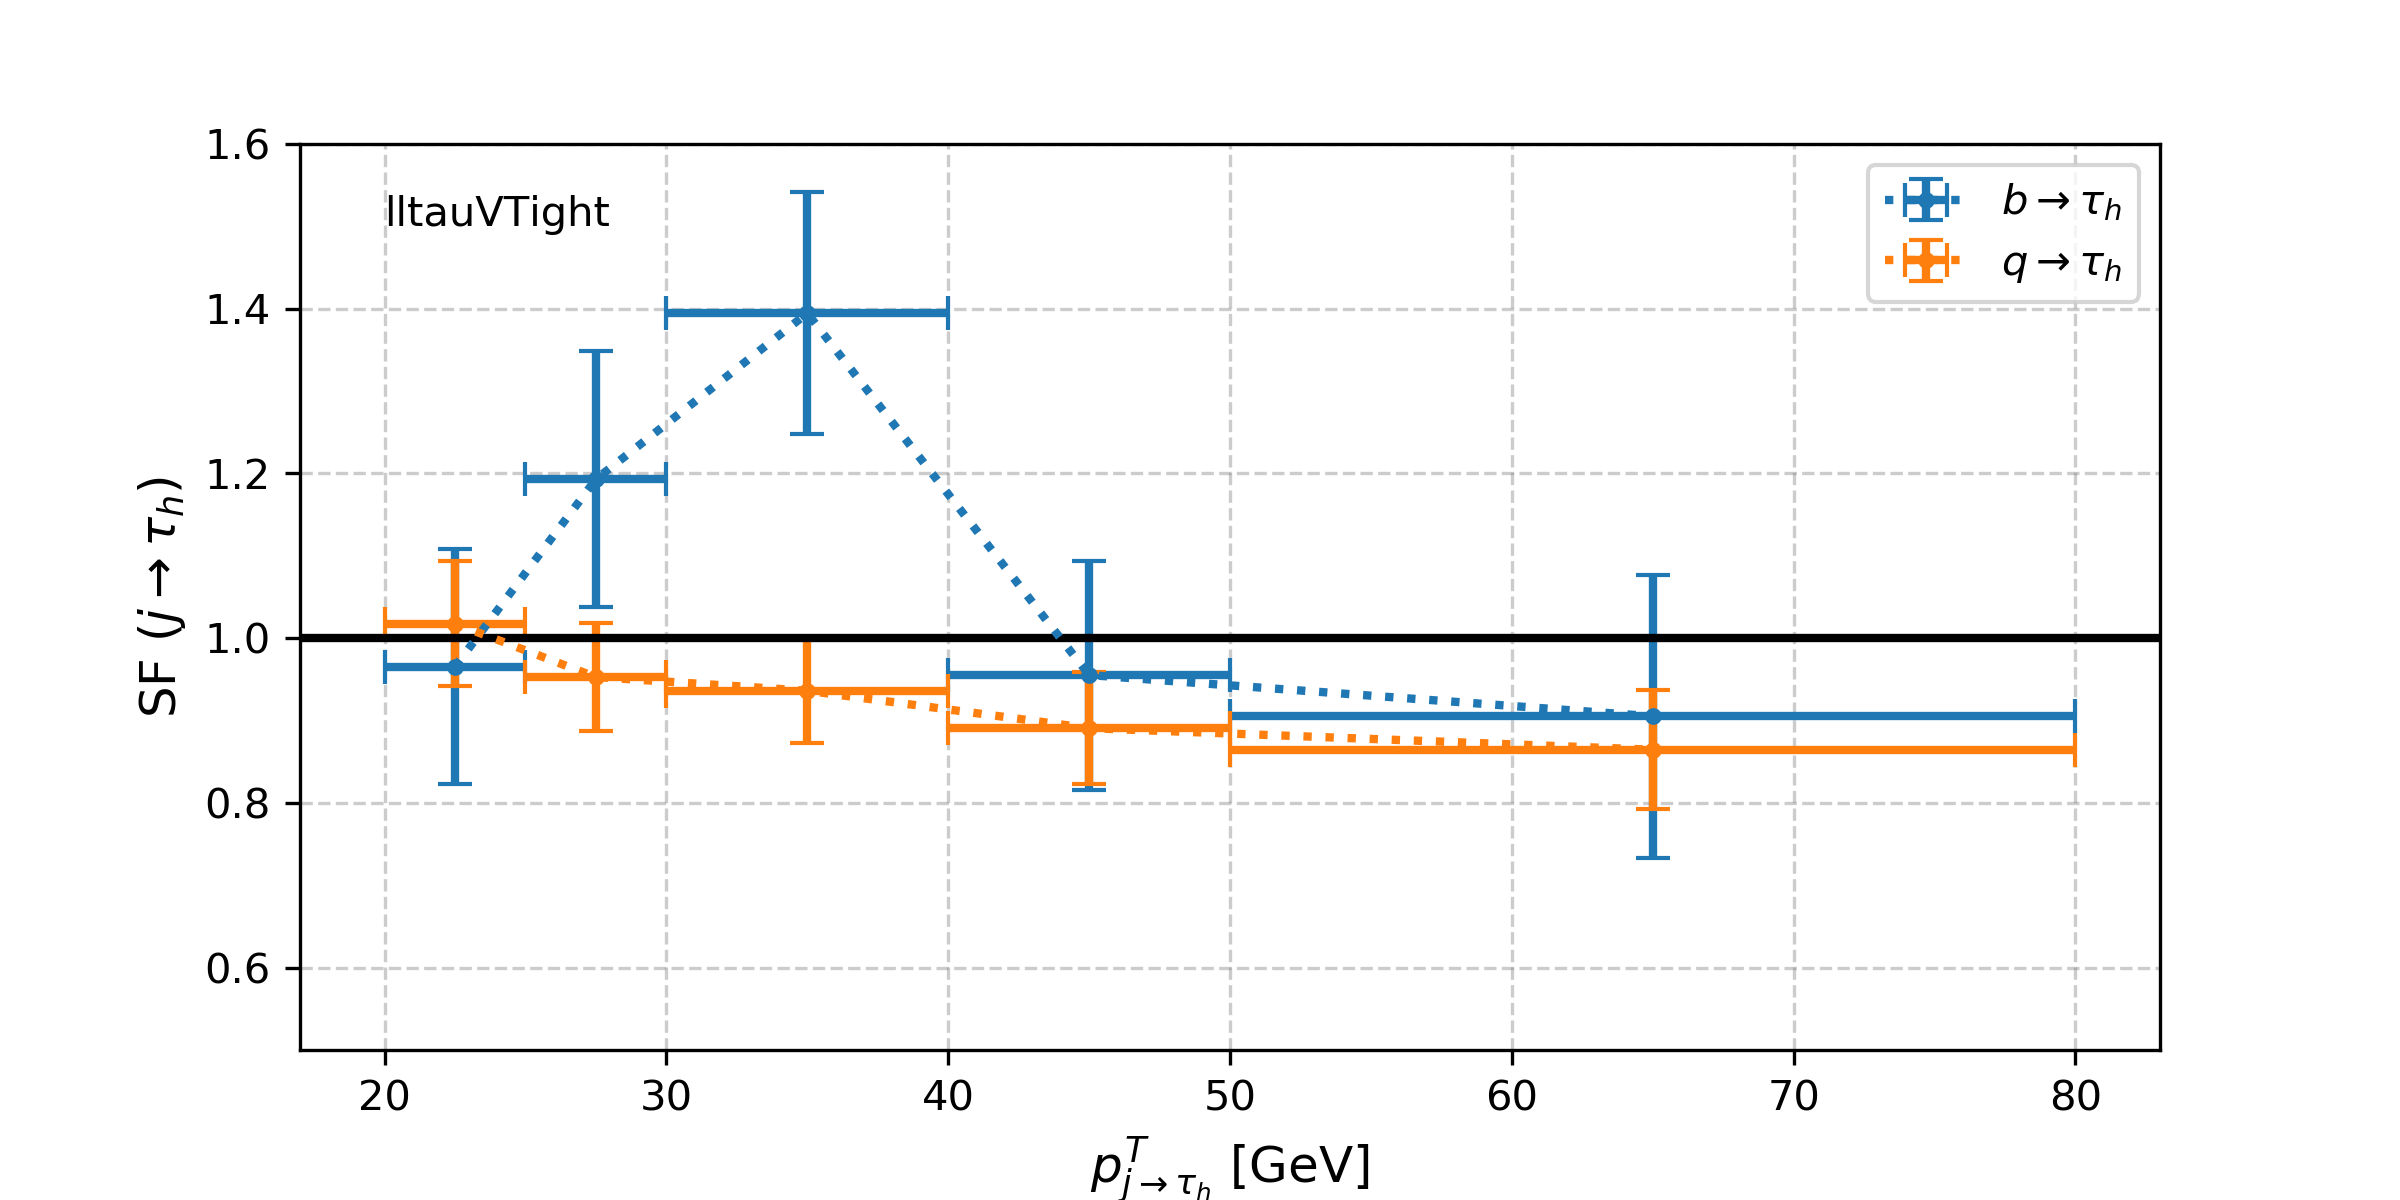
\includegraphics[width=0.49\textwidth]{chapters/Analysis/sectionCalibration/figures/jetToTauh/fit2_ptflavor2_lltauVTight.png}
    \end{block}

    
    \begin{itemize} 
        \item Fit the \pt distribution of \PGth.
        \item Free parameters for $SF_{\PQq\to \PGth}(\pt)$ and $SF_{\PQb\to \PGth}(\pt)$ in six \pt bins
        \item Systematic parameters considered 
        \begin{itemize} 
            \smaller
            \item luminosity (2.5\% error)
            \item cross-sections of \ttbar (5\%), \zjets (5\%), \wjets (5\%), diboson (10\%)
            \item reconstruction efficiencies of electron (2\%) and muon (1\%)
        \end{itemize} 
        \item Systematic parameters are Gaussian regularized by their assumed uncertainties.
    \end{itemize}
\end{frame}


\begin{frame}{}
\smaller
    \begin{center}
    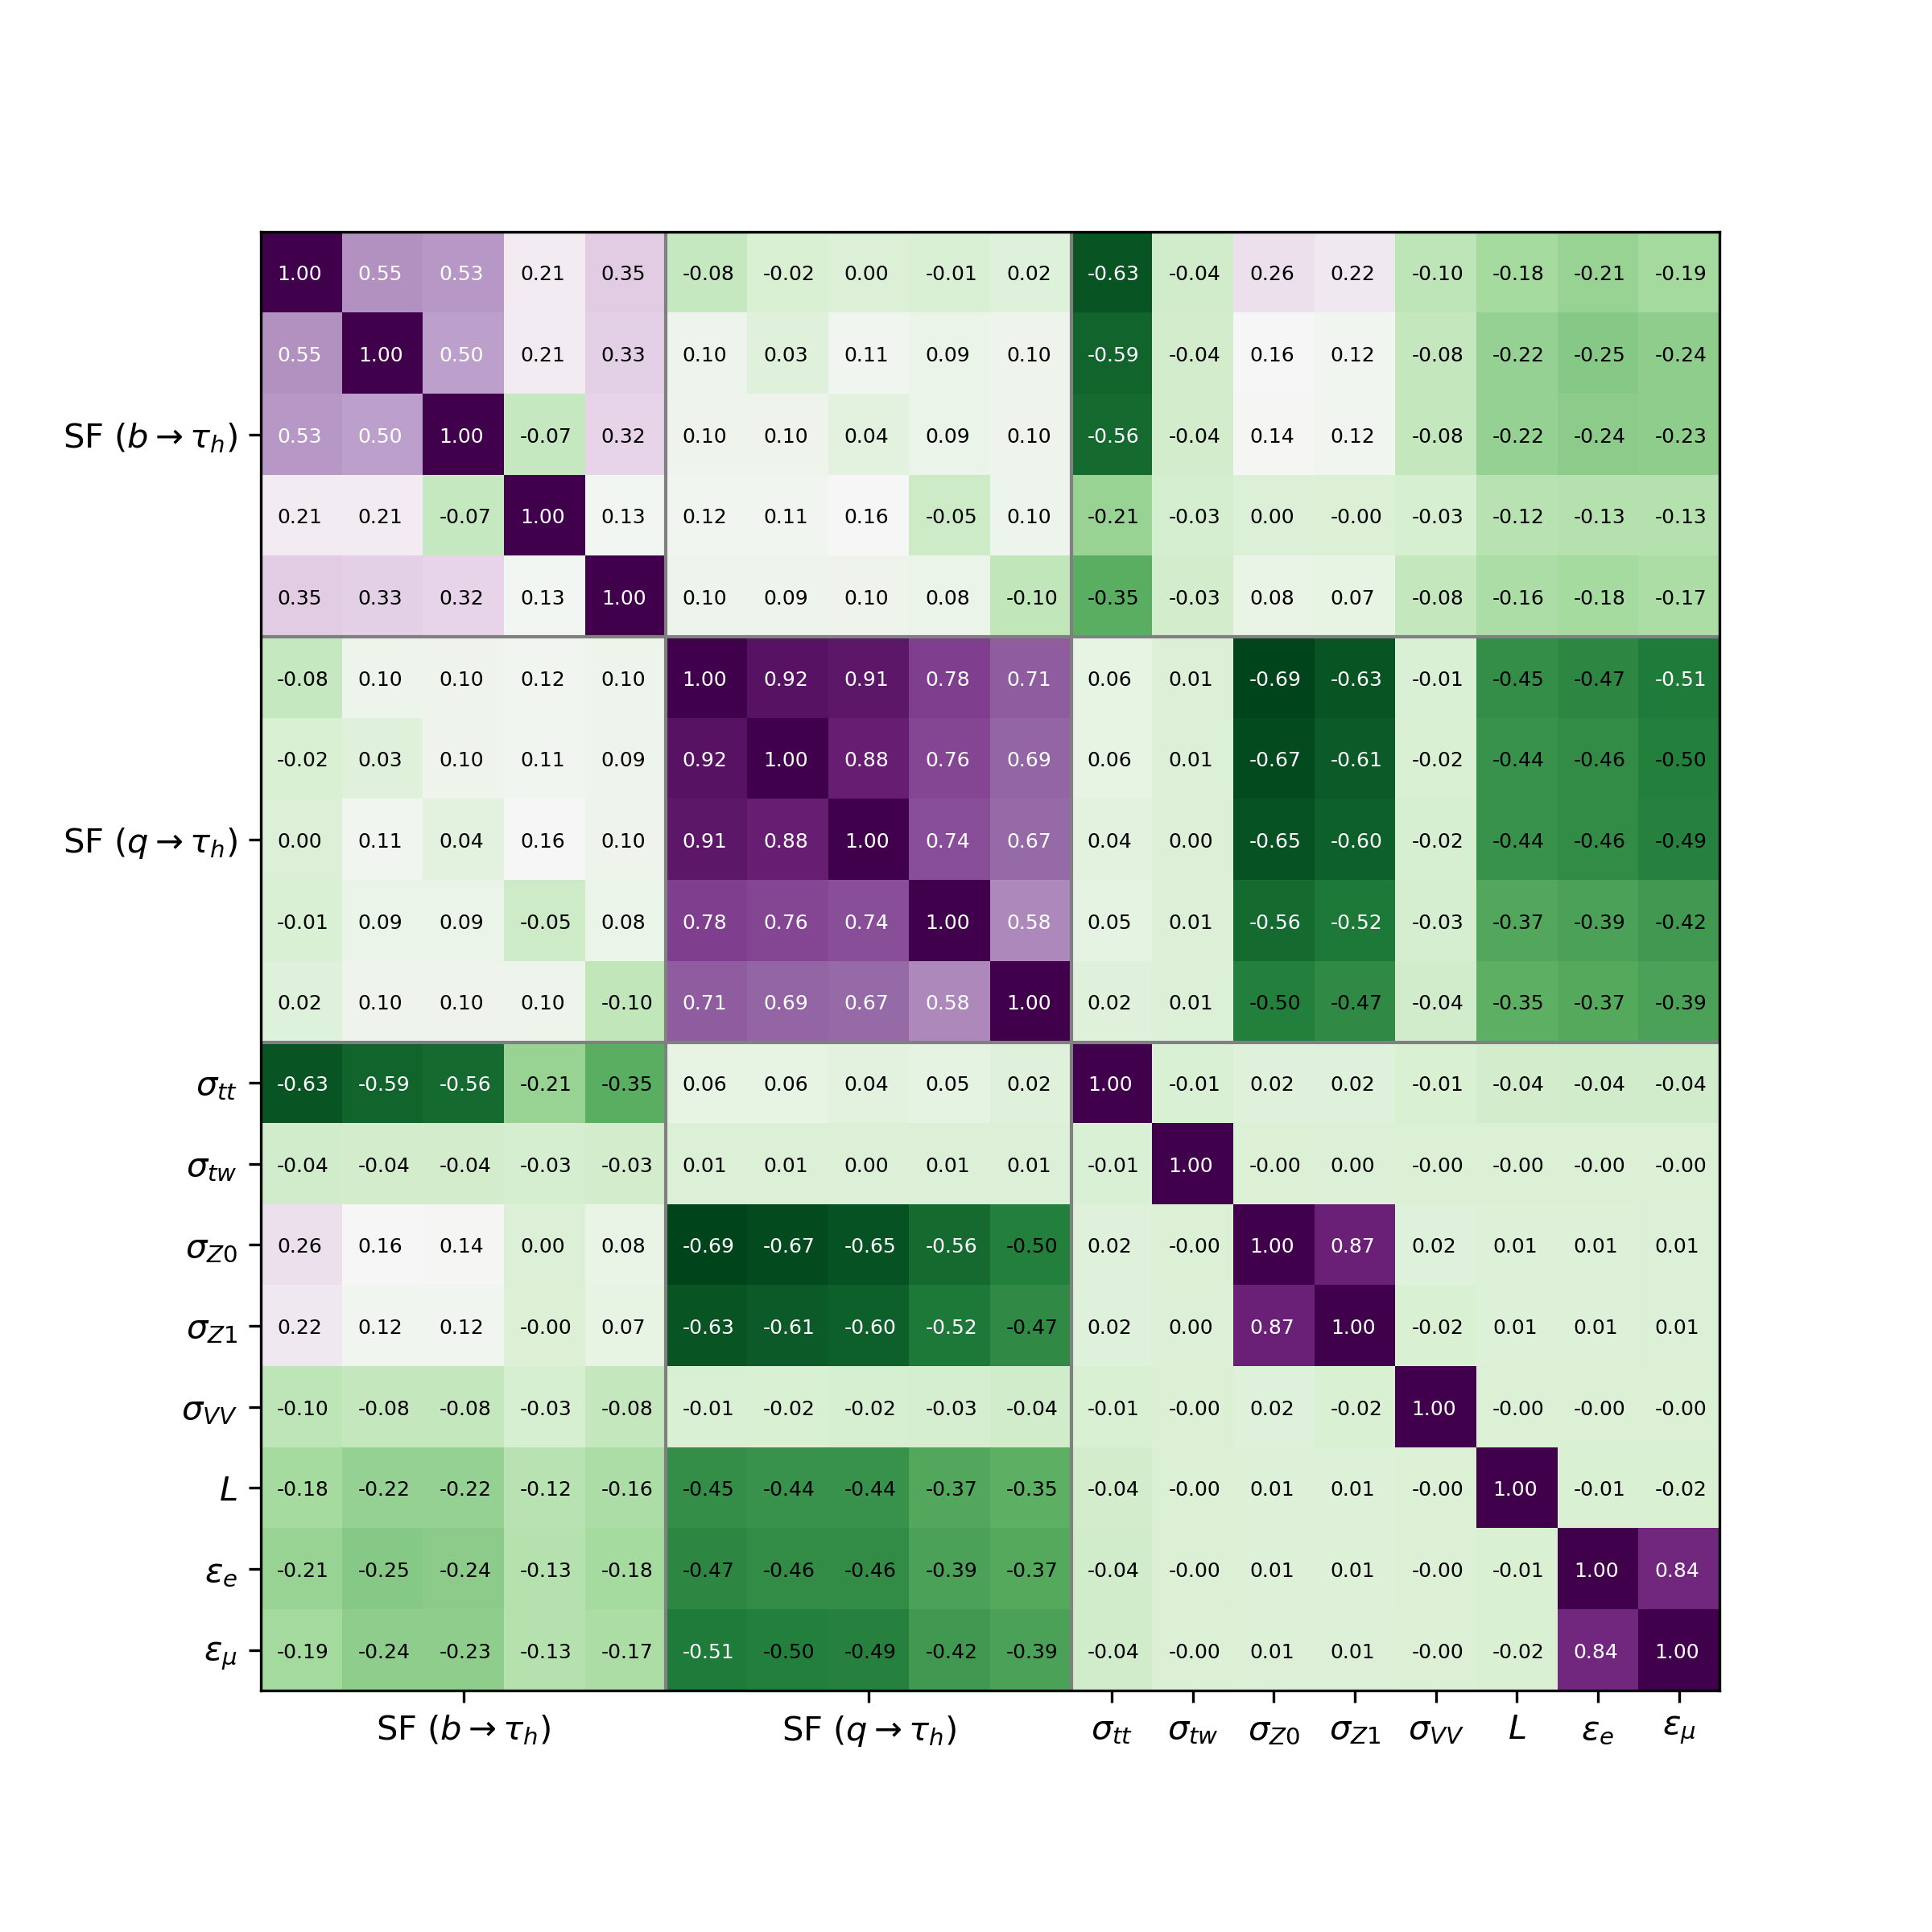
\includegraphics[width=0.4\textwidth]{chapters/Analysis/sectionCalibration/figures/jetToTauh/corr2_lltauTight_splitJetFlavor.png}
    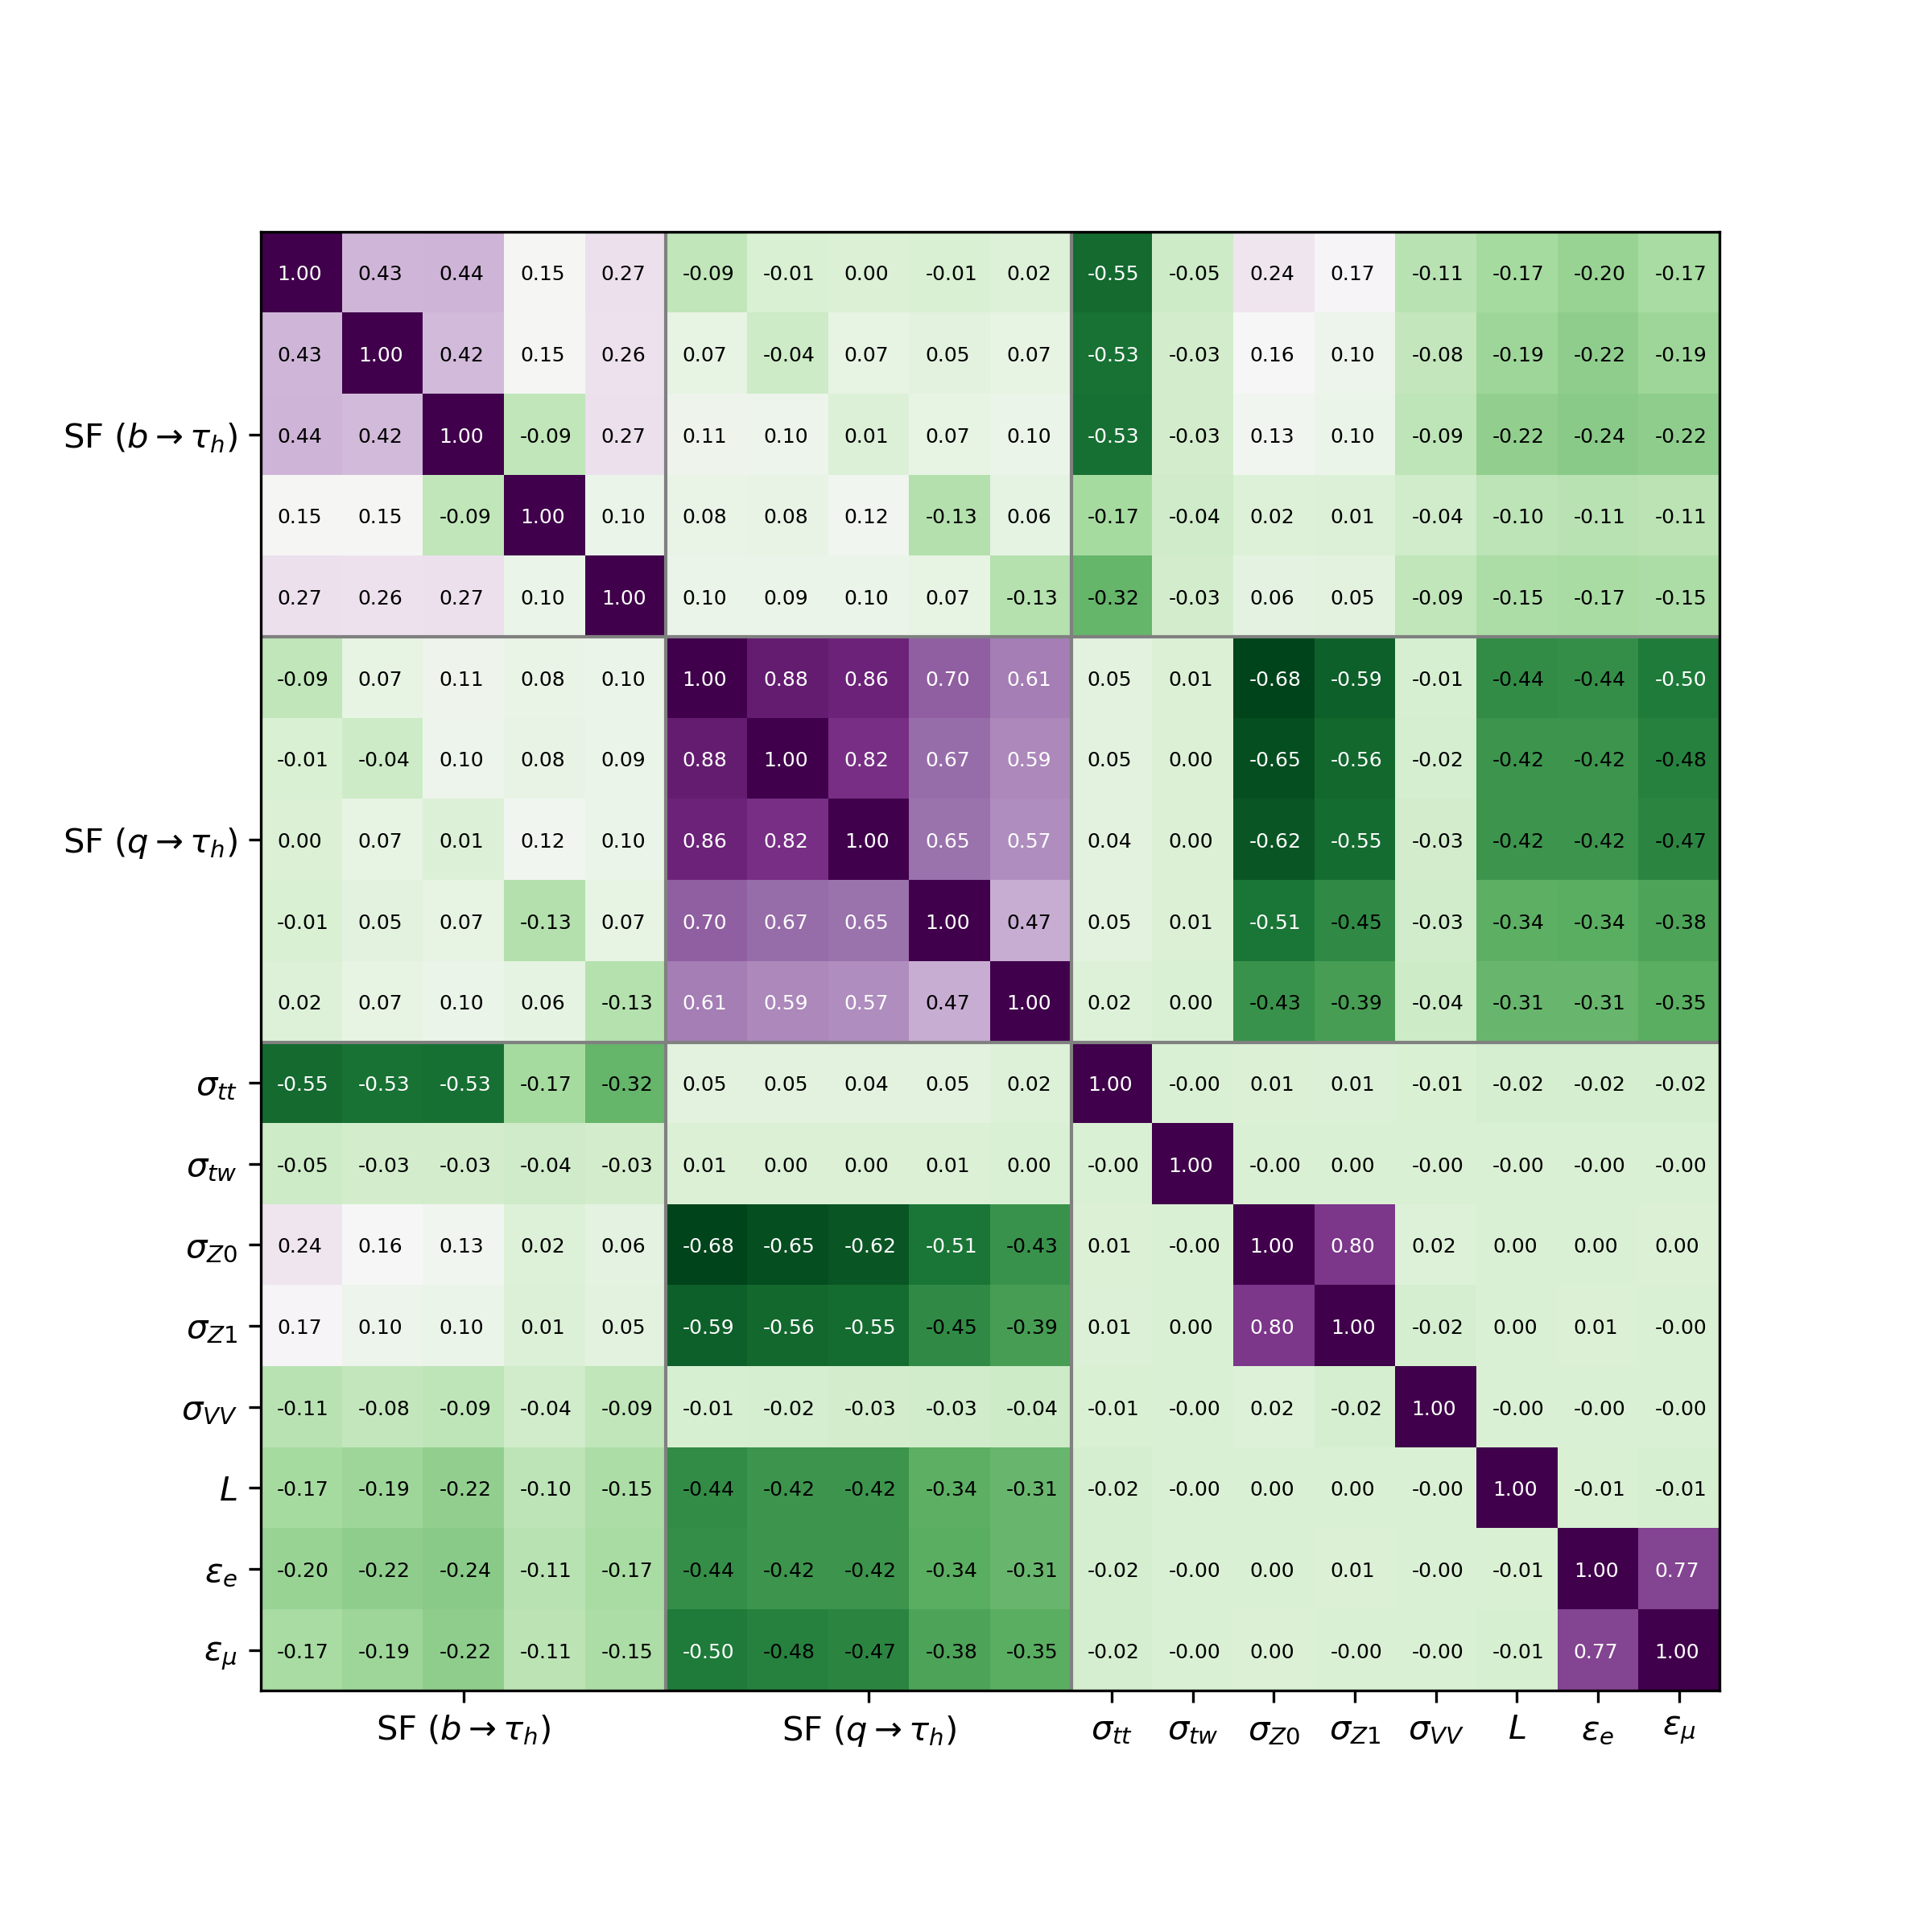
\includegraphics[width=0.4\textwidth]{chapters/Analysis/sectionCalibration/figures/jetToTauh/corr2_lltauVTight_splitJetFlavor.png}
    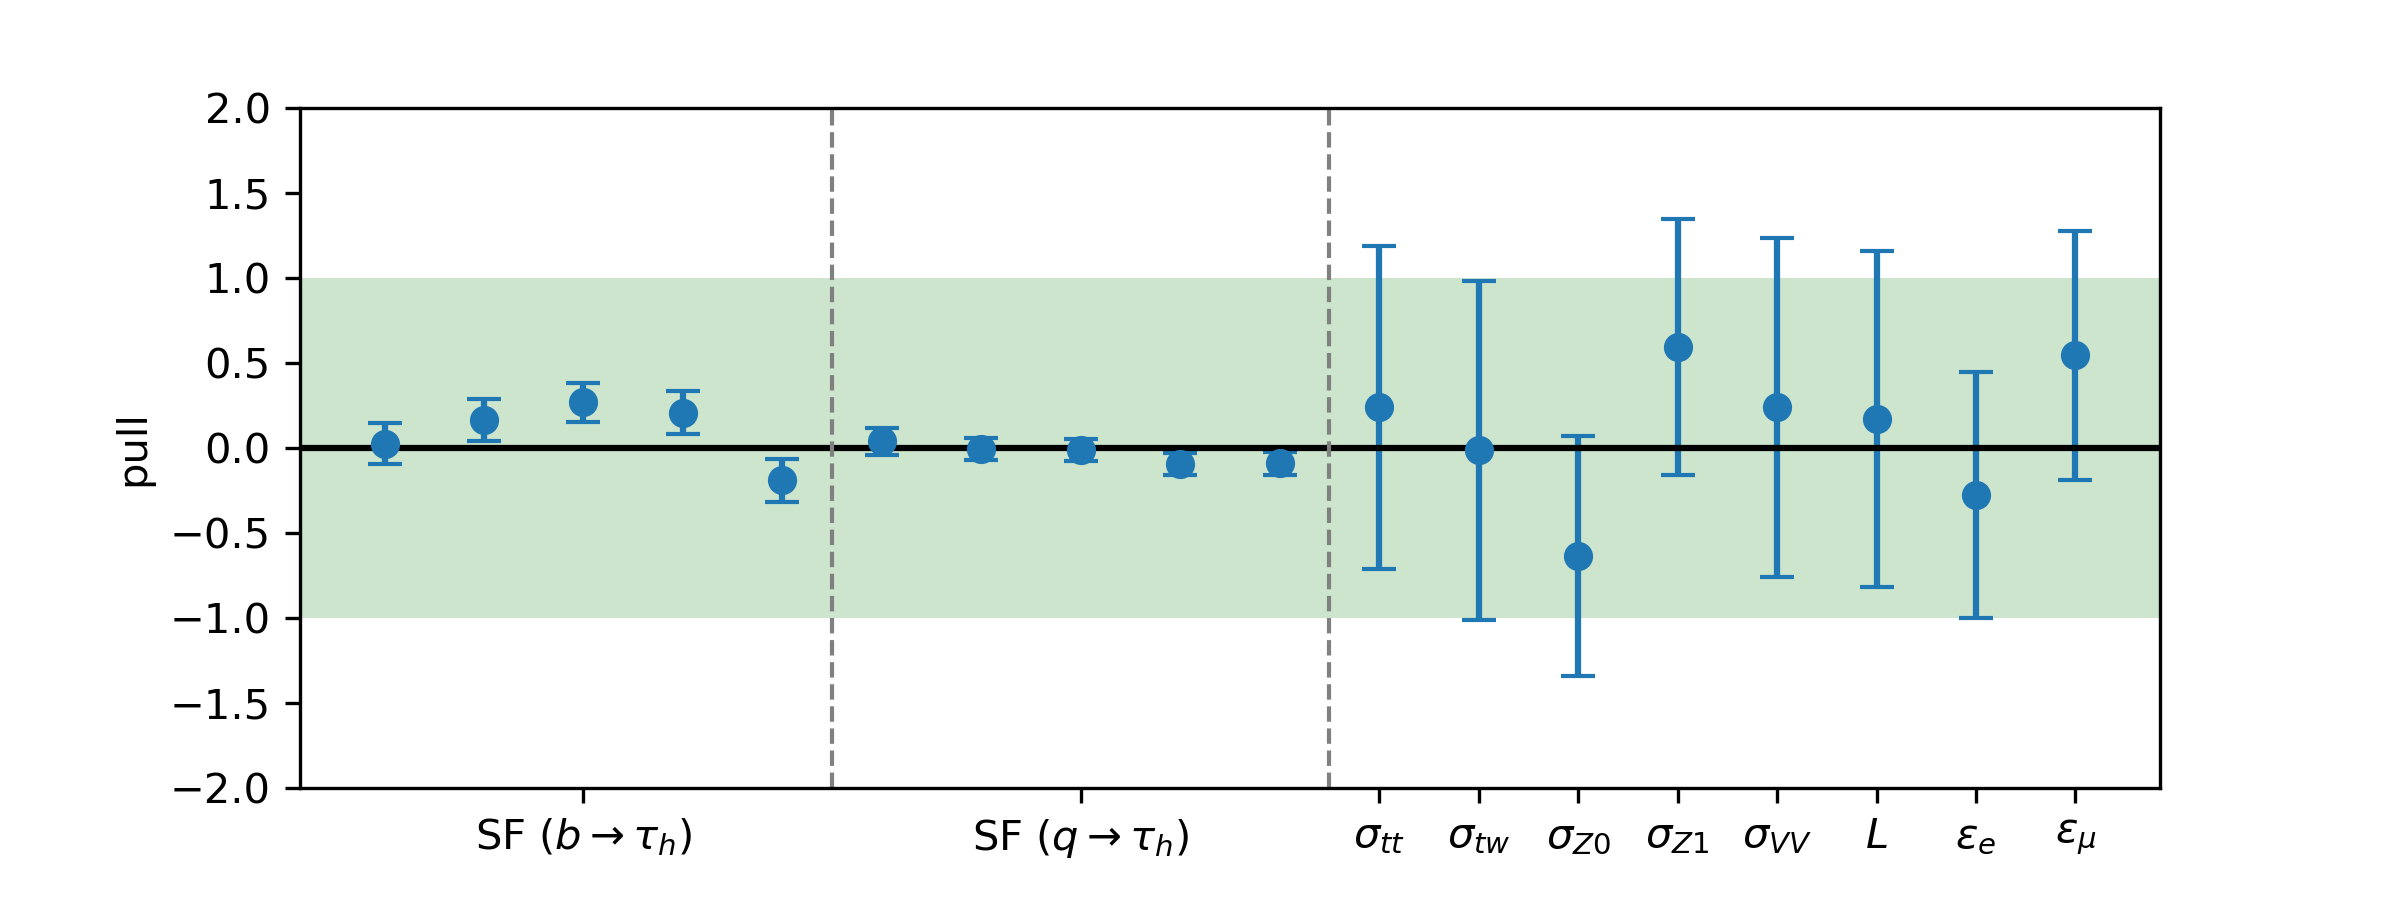
\includegraphics[width=0.4\textwidth]{chapters/Analysis/sectionCalibration/figures/jetToTauh/pull2_lltauTight_splitJetFlavor.png}
    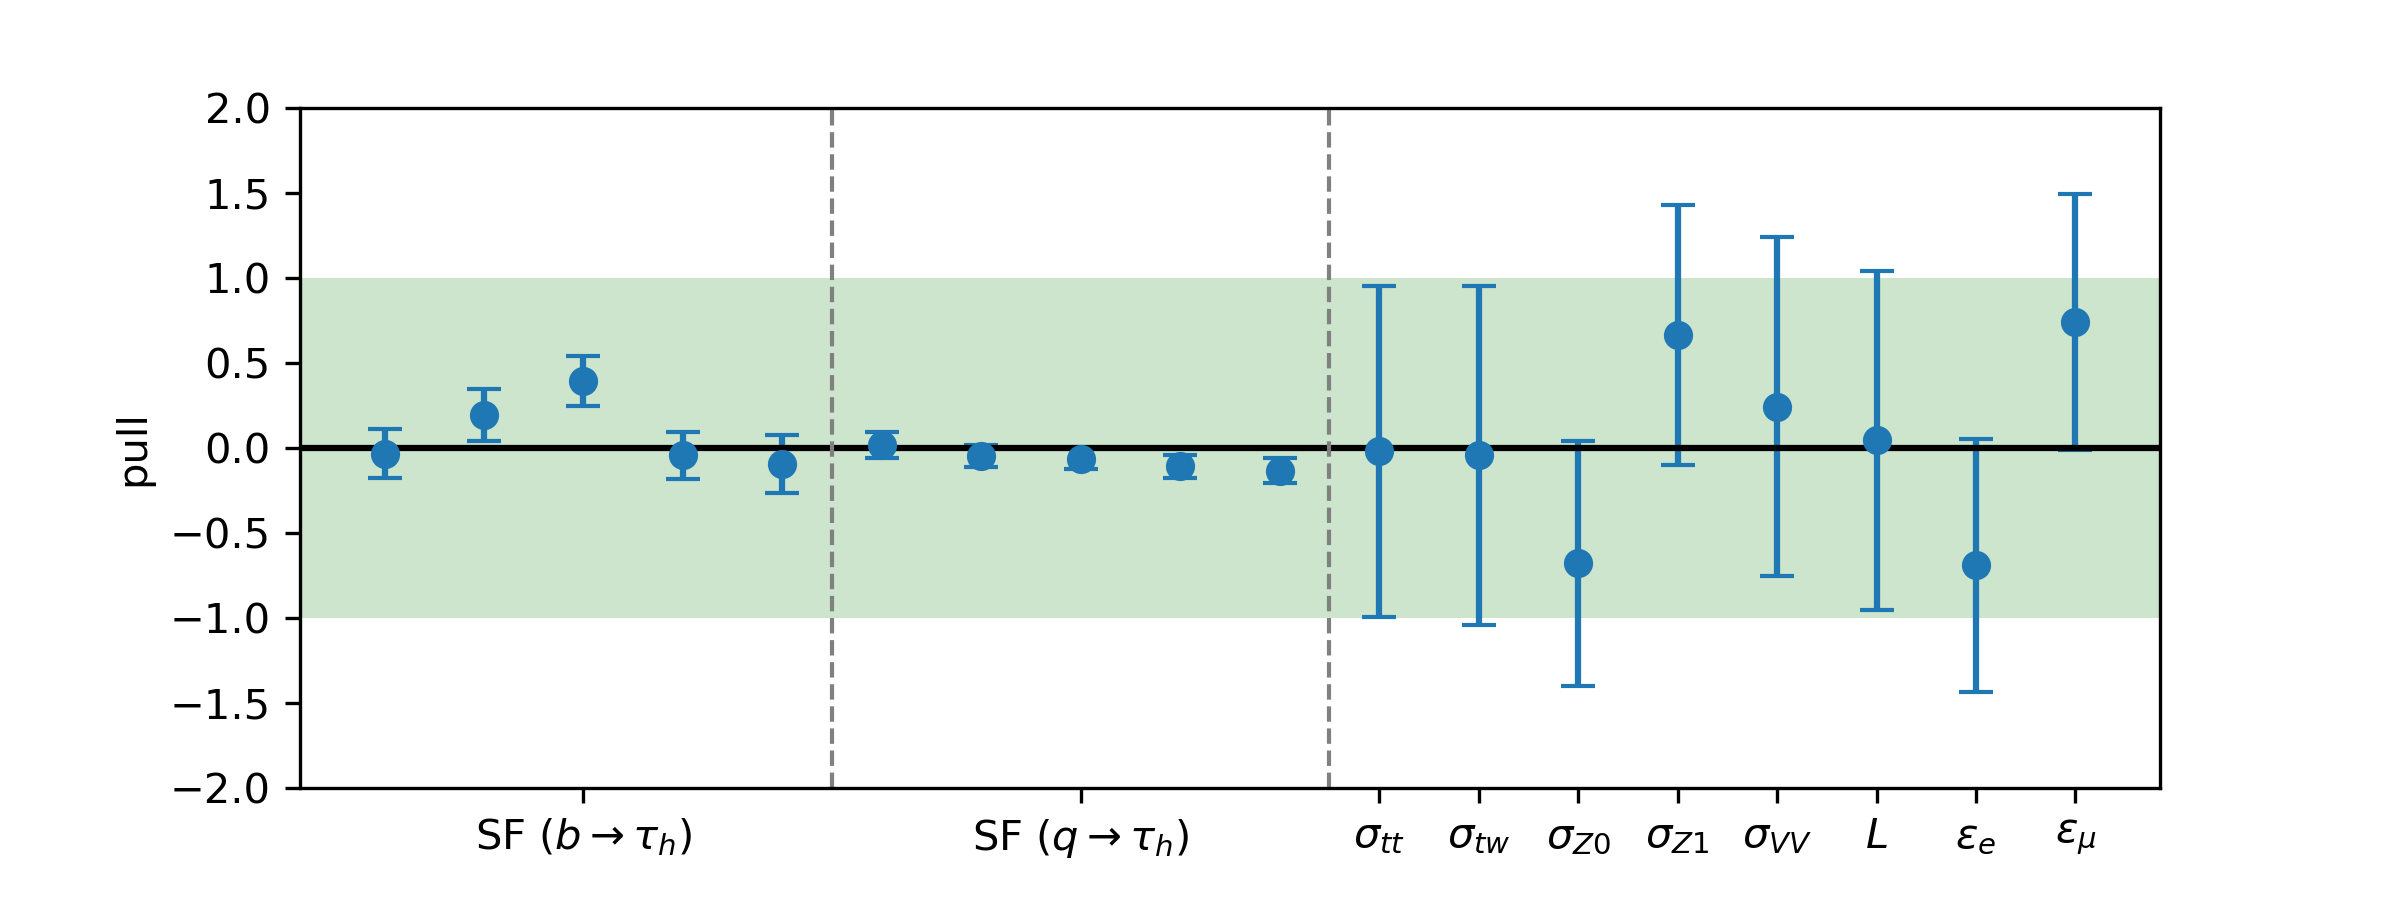
\includegraphics[width=0.4\textwidth]{chapters/Analysis/sectionCalibration/figures/jetToTauh/pull2_lltauVTight_splitJetFlavor.png}
    \end{center}
\end{frame}


% -------------
% QCD
% -------------

\begin{frame}{}
    \begin{exampleblock}{QCD in the \cmh}
    \hspace{0.12\textwidth} $SF^{\rm \overline{iso} \to iso}$ \hspace{0.3\textwidth} signal region \\
    \centering
        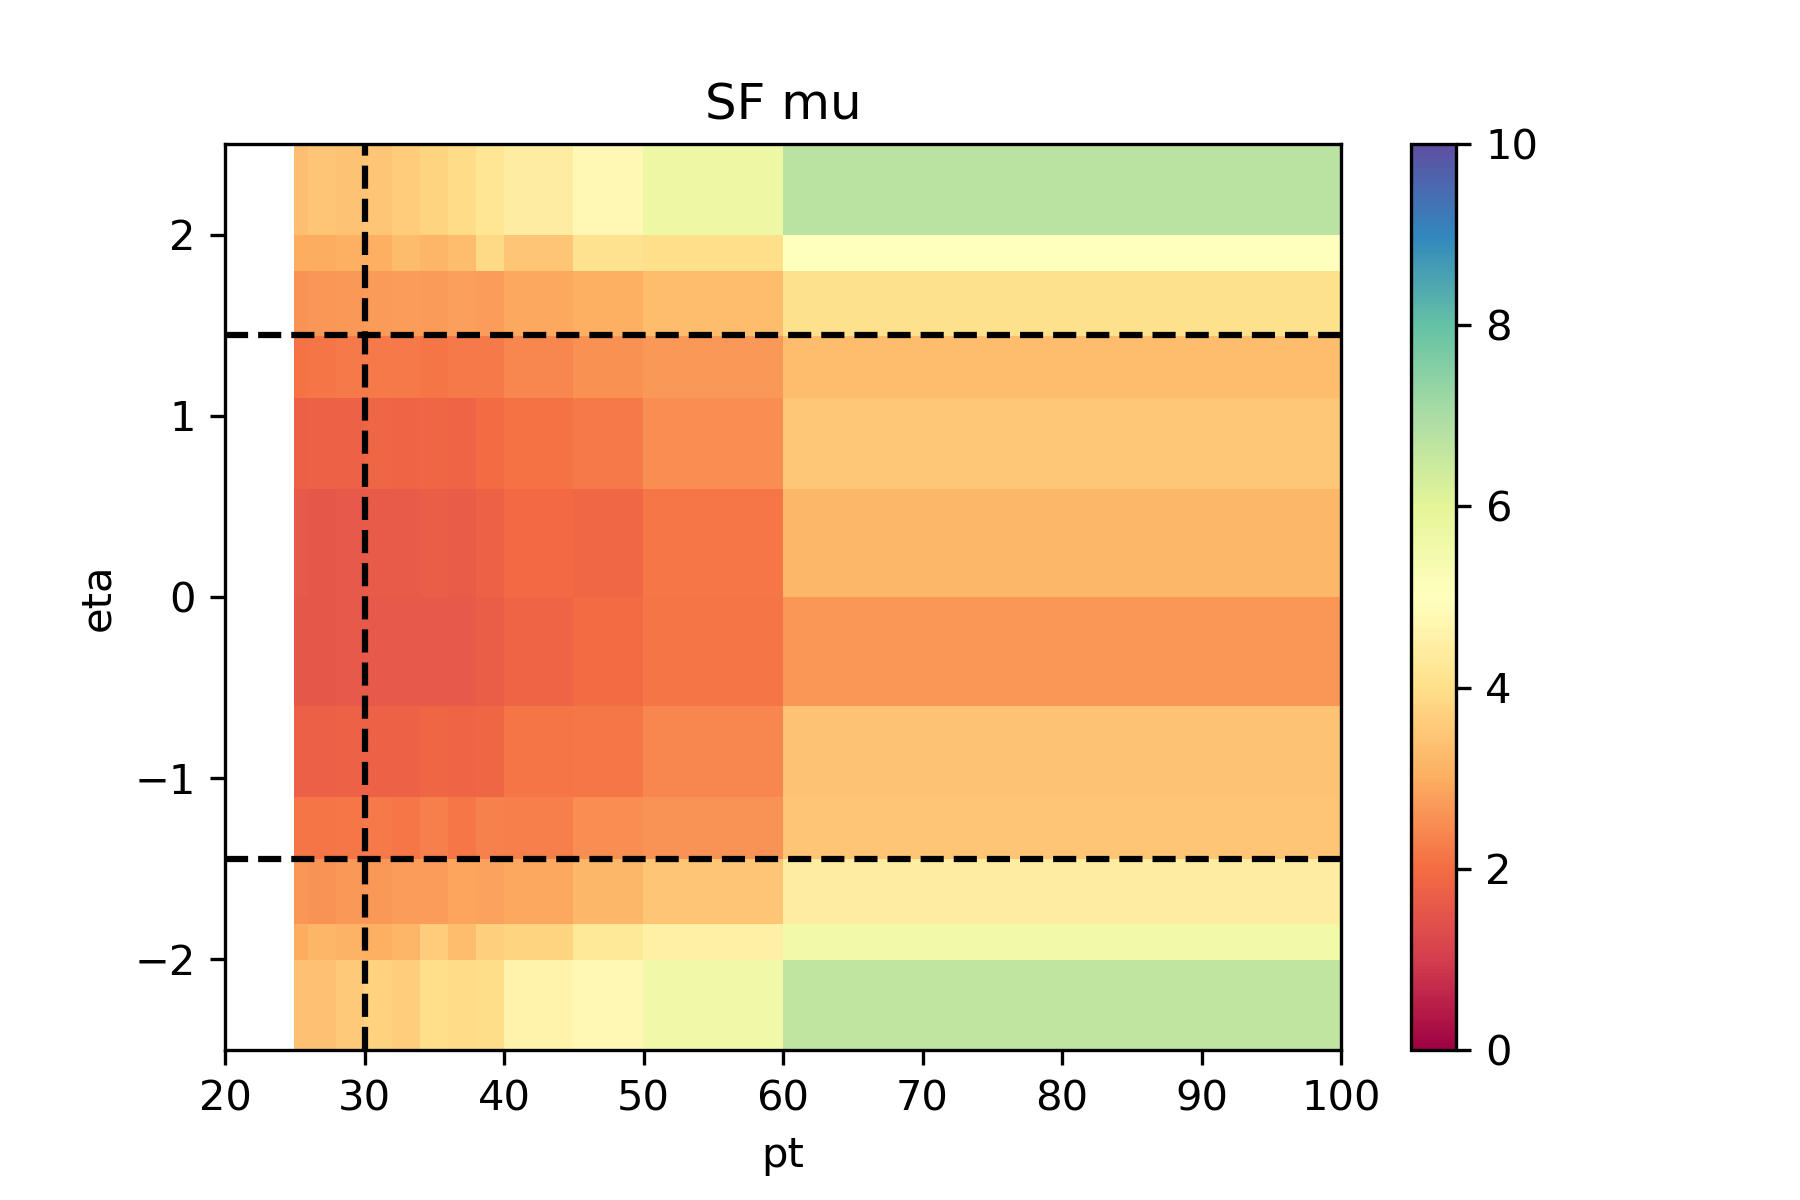
\includegraphics[height=0.32\textheight]{chapters/Analysis/sectionBackground/figures/ljets_kinematics/123j1b/SF_mu_2d.png}
        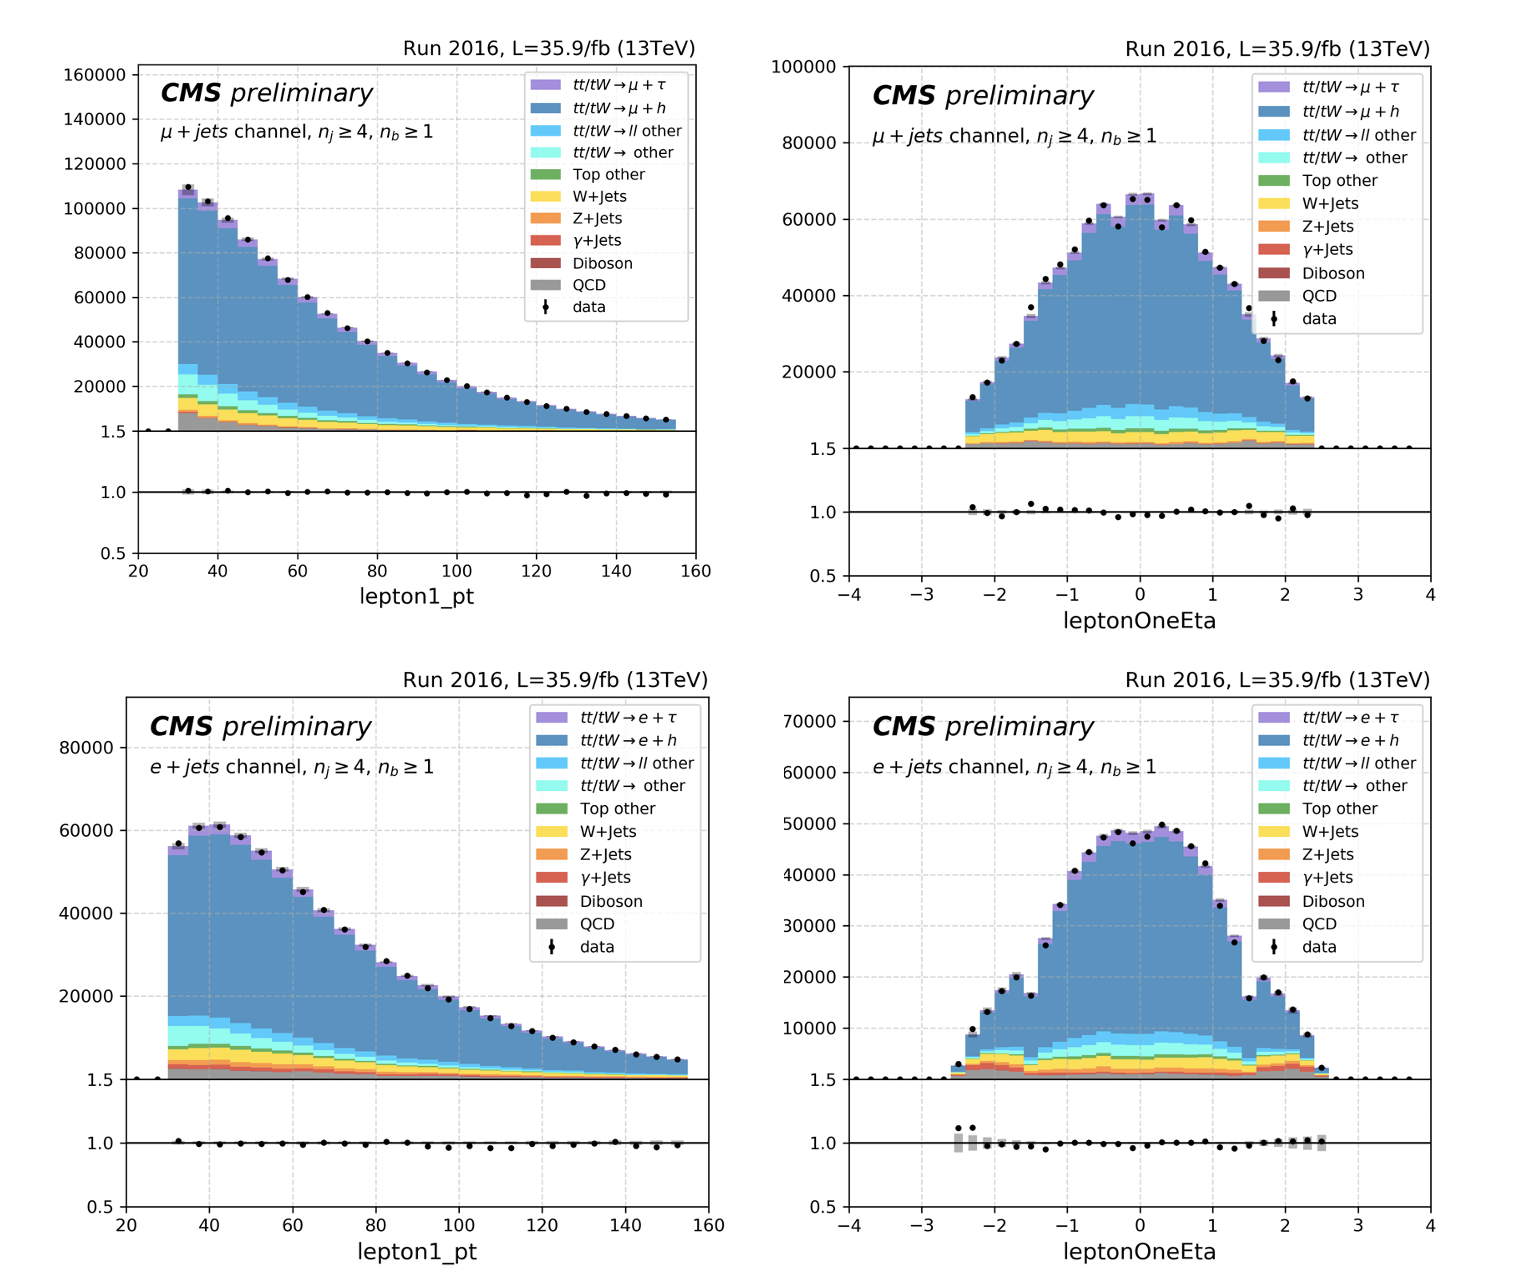
\includegraphics[height=0.32\textheight, trim=0 11cm 0 0, clip]{chapters/Analysis/sectionBackground/figures/ljets_application/mcNorm_ddShape.png}
    \end{exampleblock}
    
    \begin{exampleblock}{QCD in the \ceh}
    \hspace{0.12\textwidth} $SF^{\rm \overline{iso} \to iso}$ \hspace{0.3\textwidth} signal region \\
    \centering
        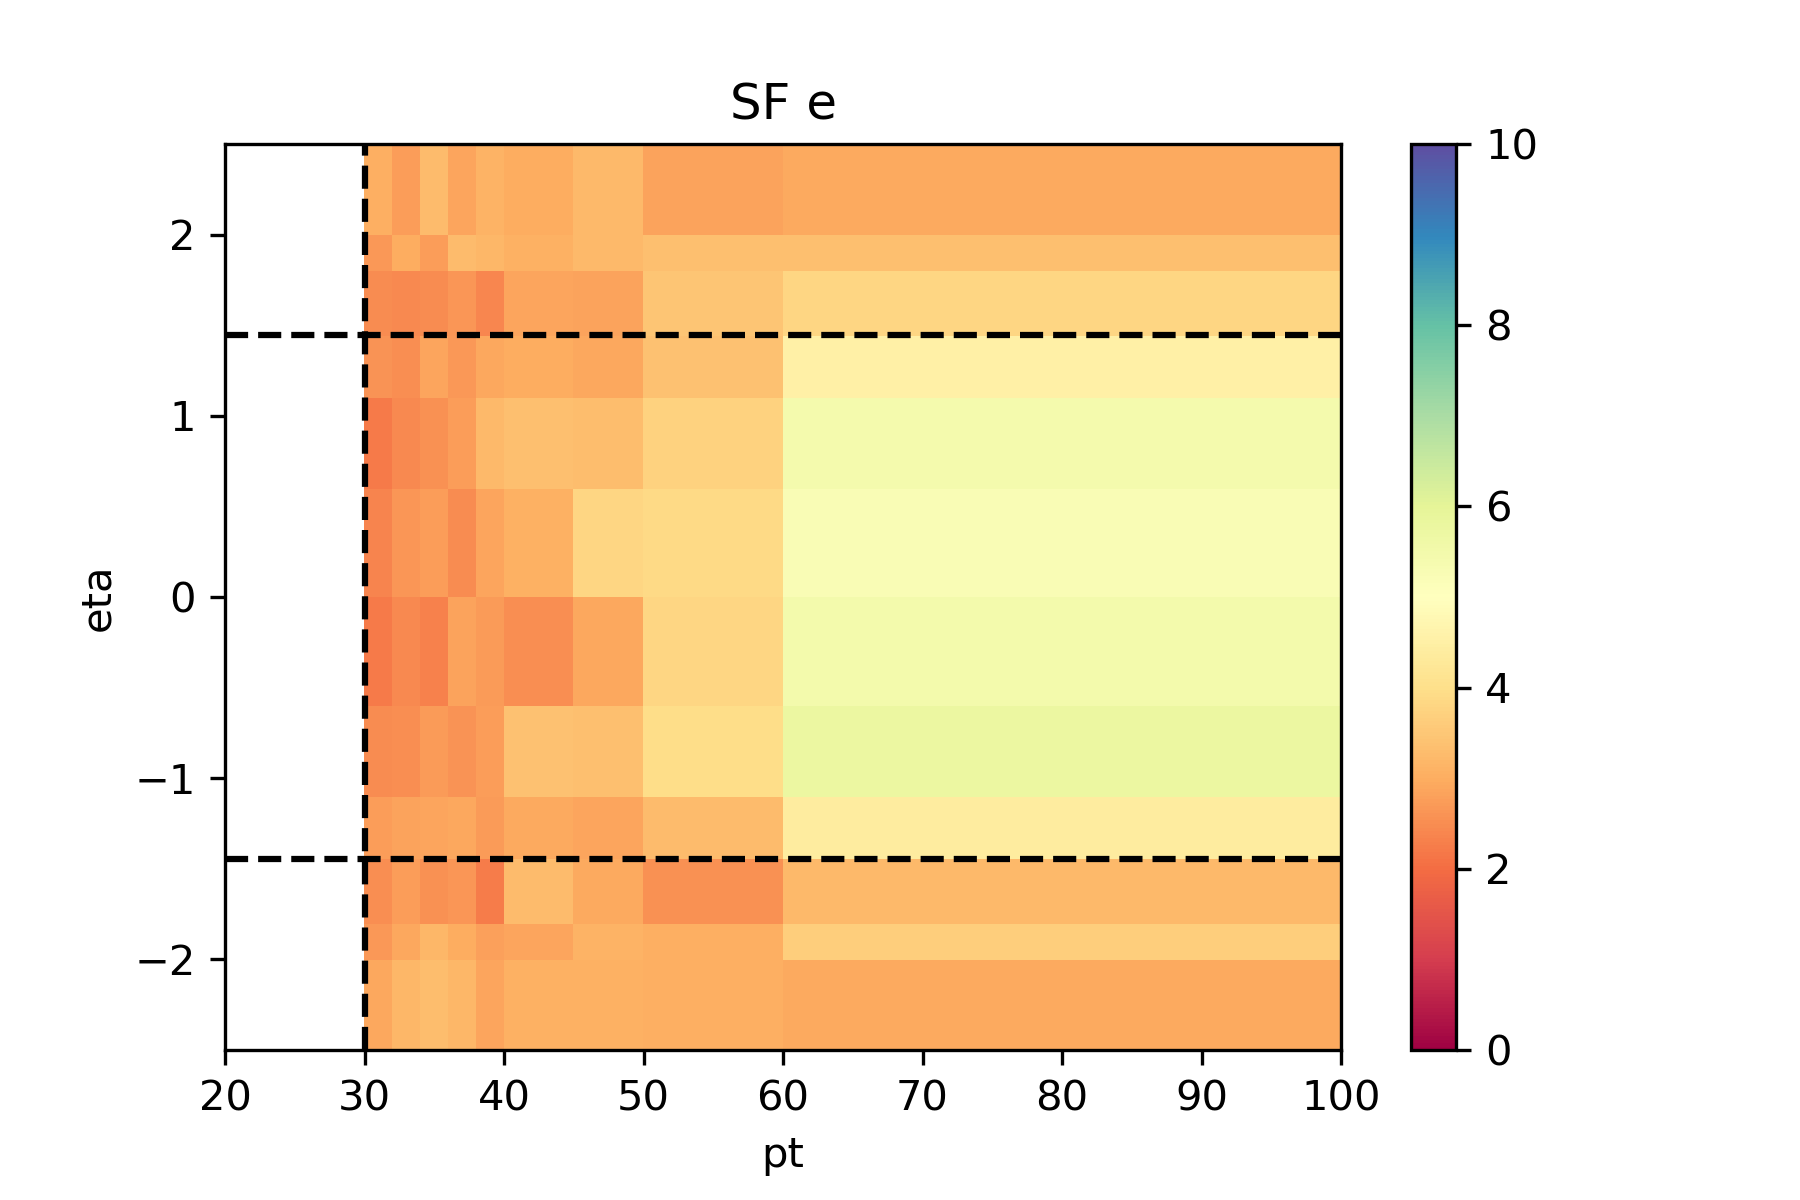
\includegraphics[height=0.32\textheight]{chapters/Analysis/sectionBackground/figures/ljets_kinematics/123j1b/SF_e_2d.png}
        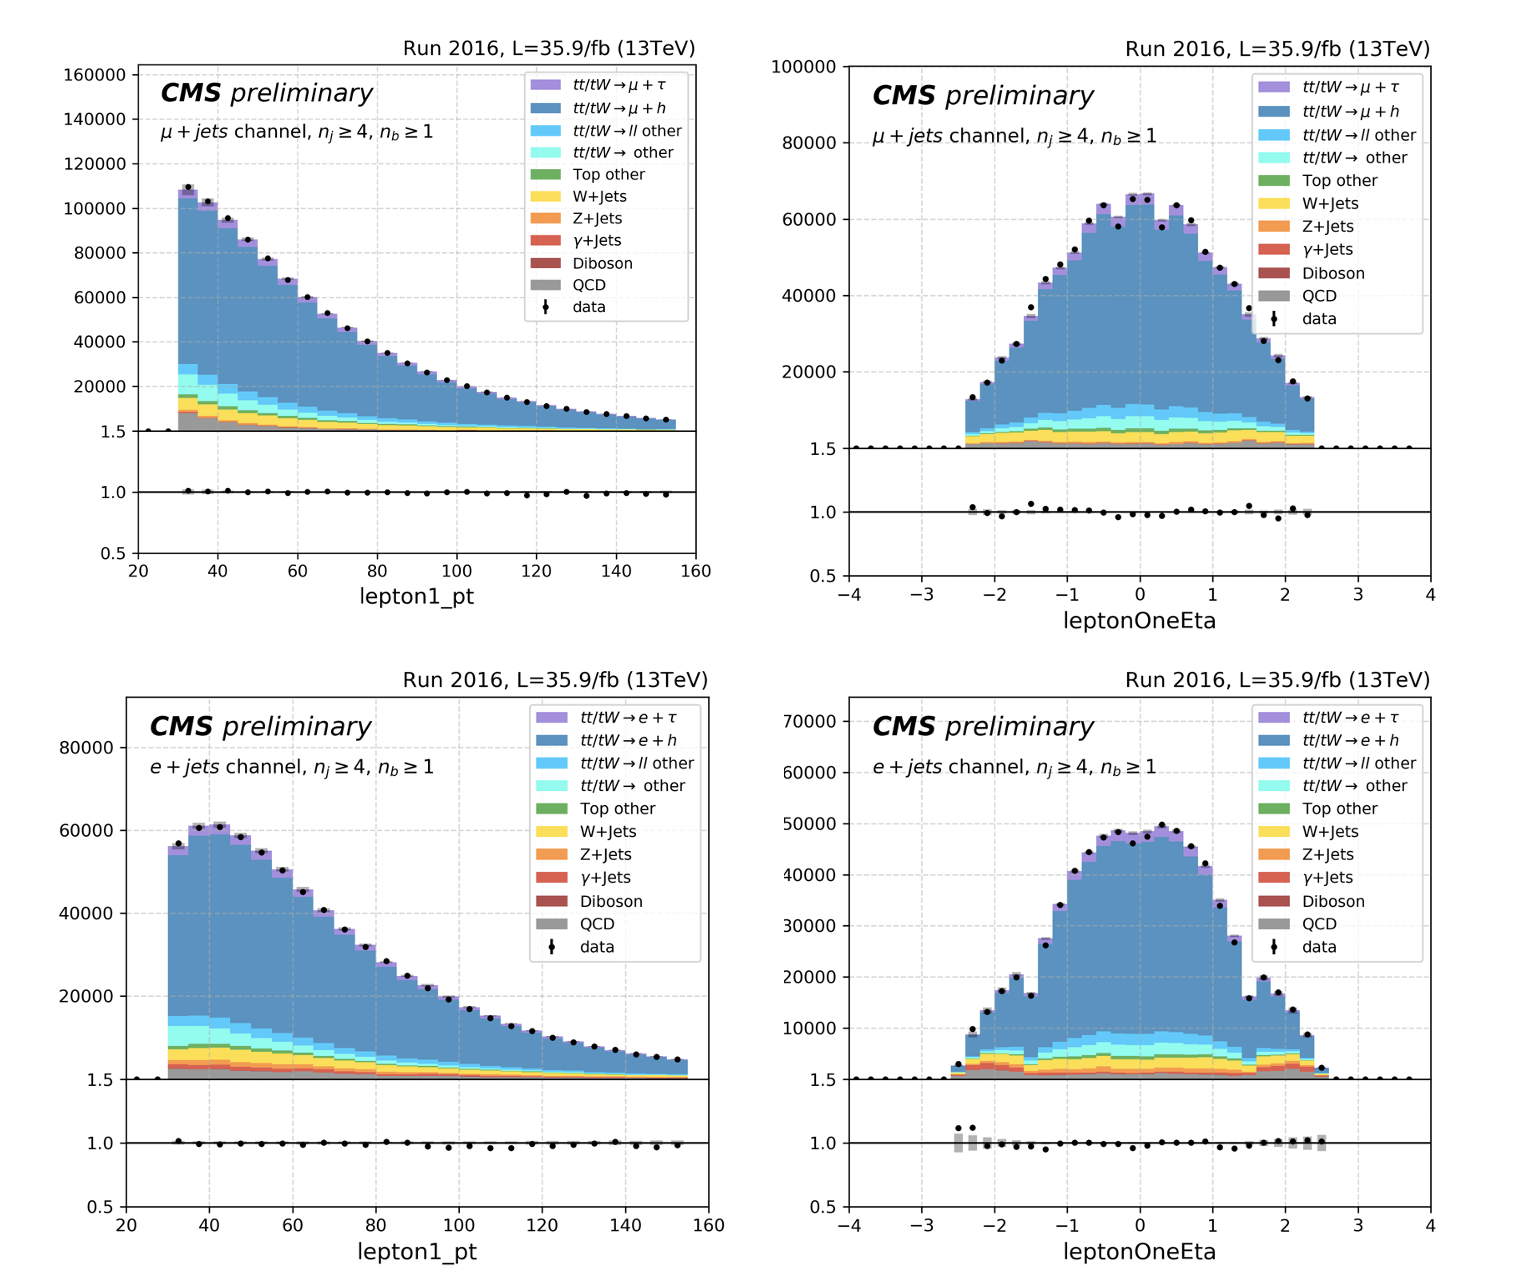
\includegraphics[height=0.32\textheight, trim=0 0 0 11.2cm, clip]{chapters/Analysis/sectionBackground/figures/ljets_application/mcNorm_ddShape.png}
    \end{exampleblock}

\end{frame}


% -------------
% Systematics
% -------------

\begin{frame}{\bth decay branching fractions}

    \begin{itemize}
    \smaller
        \item brought up in a CMS week talk.
        \item tau reconstruction efficiencies are different for different \PGth decay mode.
        \item major \PGth decay branching fractions 
            \begin{equation*}\tiny
            \begin{split}
            &   \mathcal{B}(\PGth\to \PGp^\pm)        = 0.1082(5), \quad 
                \mathcal{B}(\PGth\to \PGp^\pm \PGp^0)  = 0.2549(9), \quad 
                \mathcal{B}(\PGth\to \PGp^\pm2\PGp^0)  = 0.0926(10),\\
            &   \mathcal{B}(\PGth\to3\PGp^\pm)        = 0.0931(5), \quad
                \mathcal{B}(\PGth\to3\PGp^\pm \PGp^0)  = 0.0462(5).           
            \end{split}
            \end{equation*}
        \item find the decay mode of \PGth in simulation based on gen-level information. 
        \item propagate uncertainty of each $\mathcal{B}(\PGth)$
        \item impact less than 0.1\%. neglectable.
    \end{itemize}
        

    \begin{figure}
    \centering
    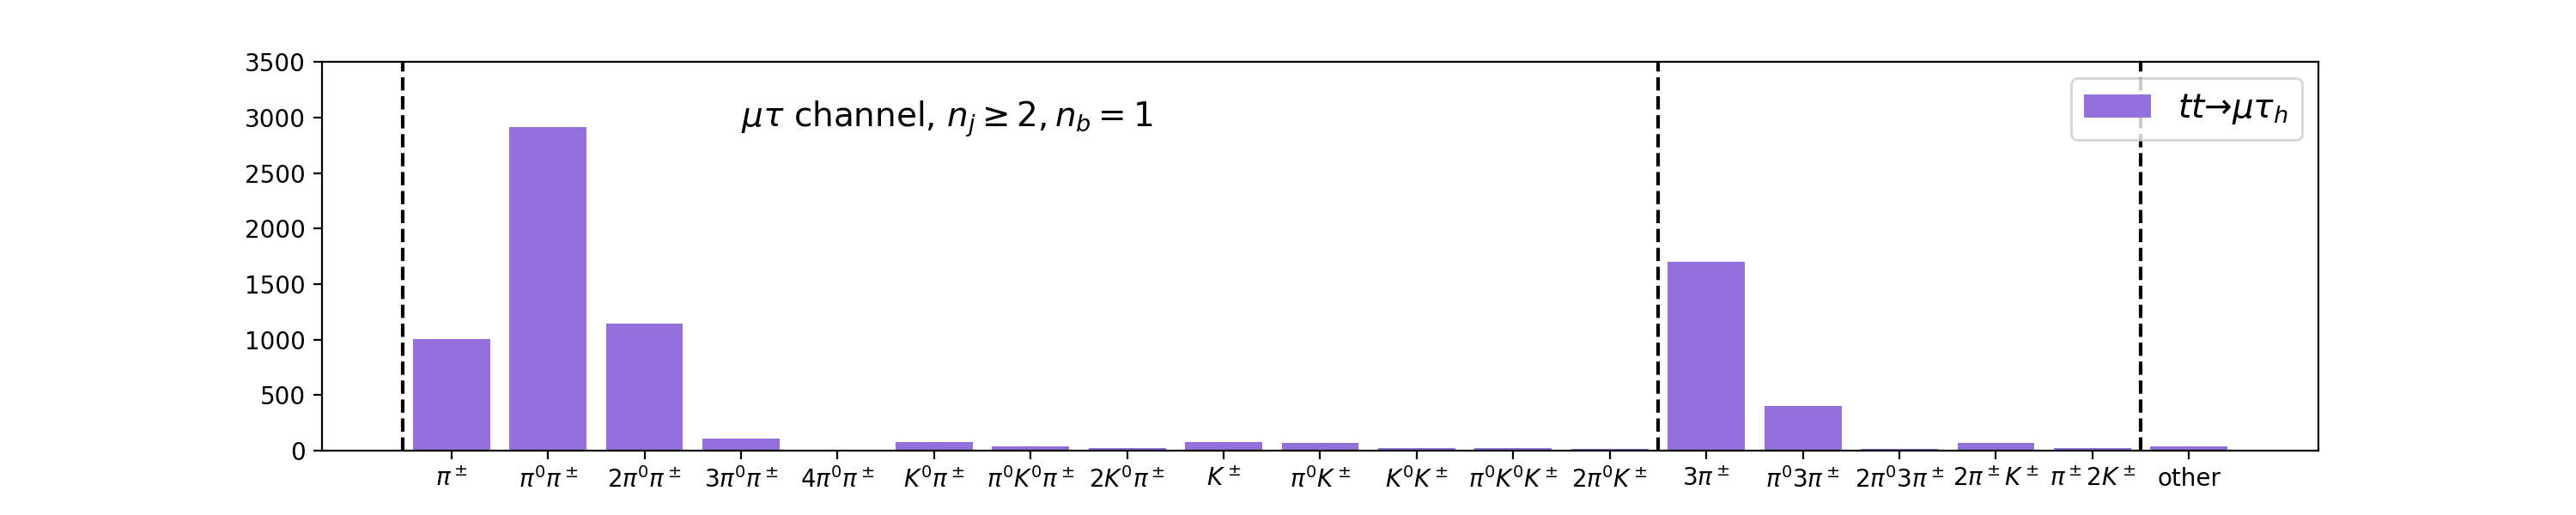
\includegraphics[width=0.99\textwidth]{chapters/Analysis/sectionSystematics/figures/tauBr/tauhDecay_mutau.png}
    \end{figure}
\end{frame}


\begin{frame}{Removal of $\PGth$ systematics from FSR}

    \begin{itemize}
    \smaller
        \item tau reconstruction is sensitive to $\alpS$ in the FSR systematics. 
        \item remove the effect of \PGth identification when evaluating FSR systematics.
        \item avoid double counting \PGth identification systematics.
        \item measure the \PGth identification efficiency in nominal and FSR+- simulation.
        \item reweight the FSR+- simulation with scale factors.
    \end{itemize}
        

    \begin{figure}
    \centering
    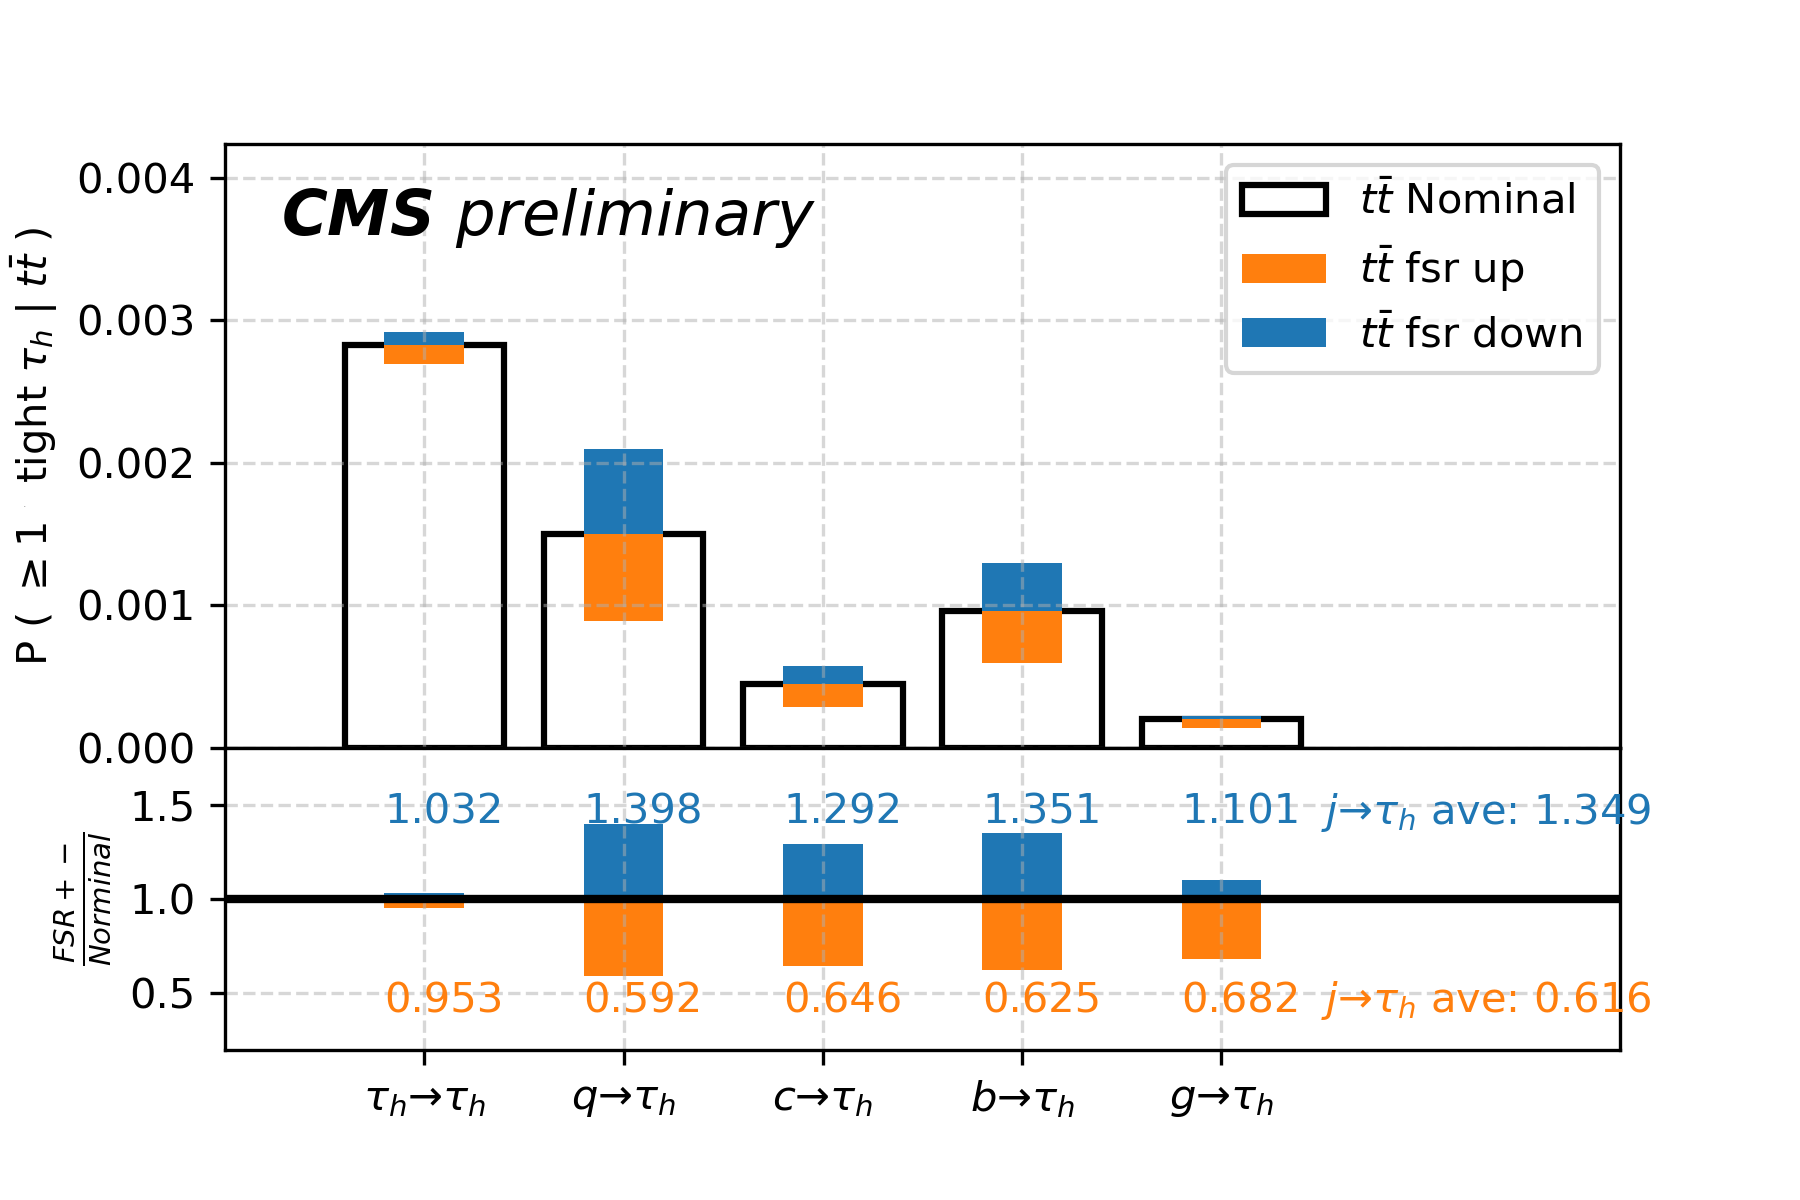
\includegraphics[width=0.49\textwidth]{chapters/Analysis/sectionSystematics/figures/ttTheoretical/2020_MCRatio_fsr_tauGenFlavor_tauTight.png}
    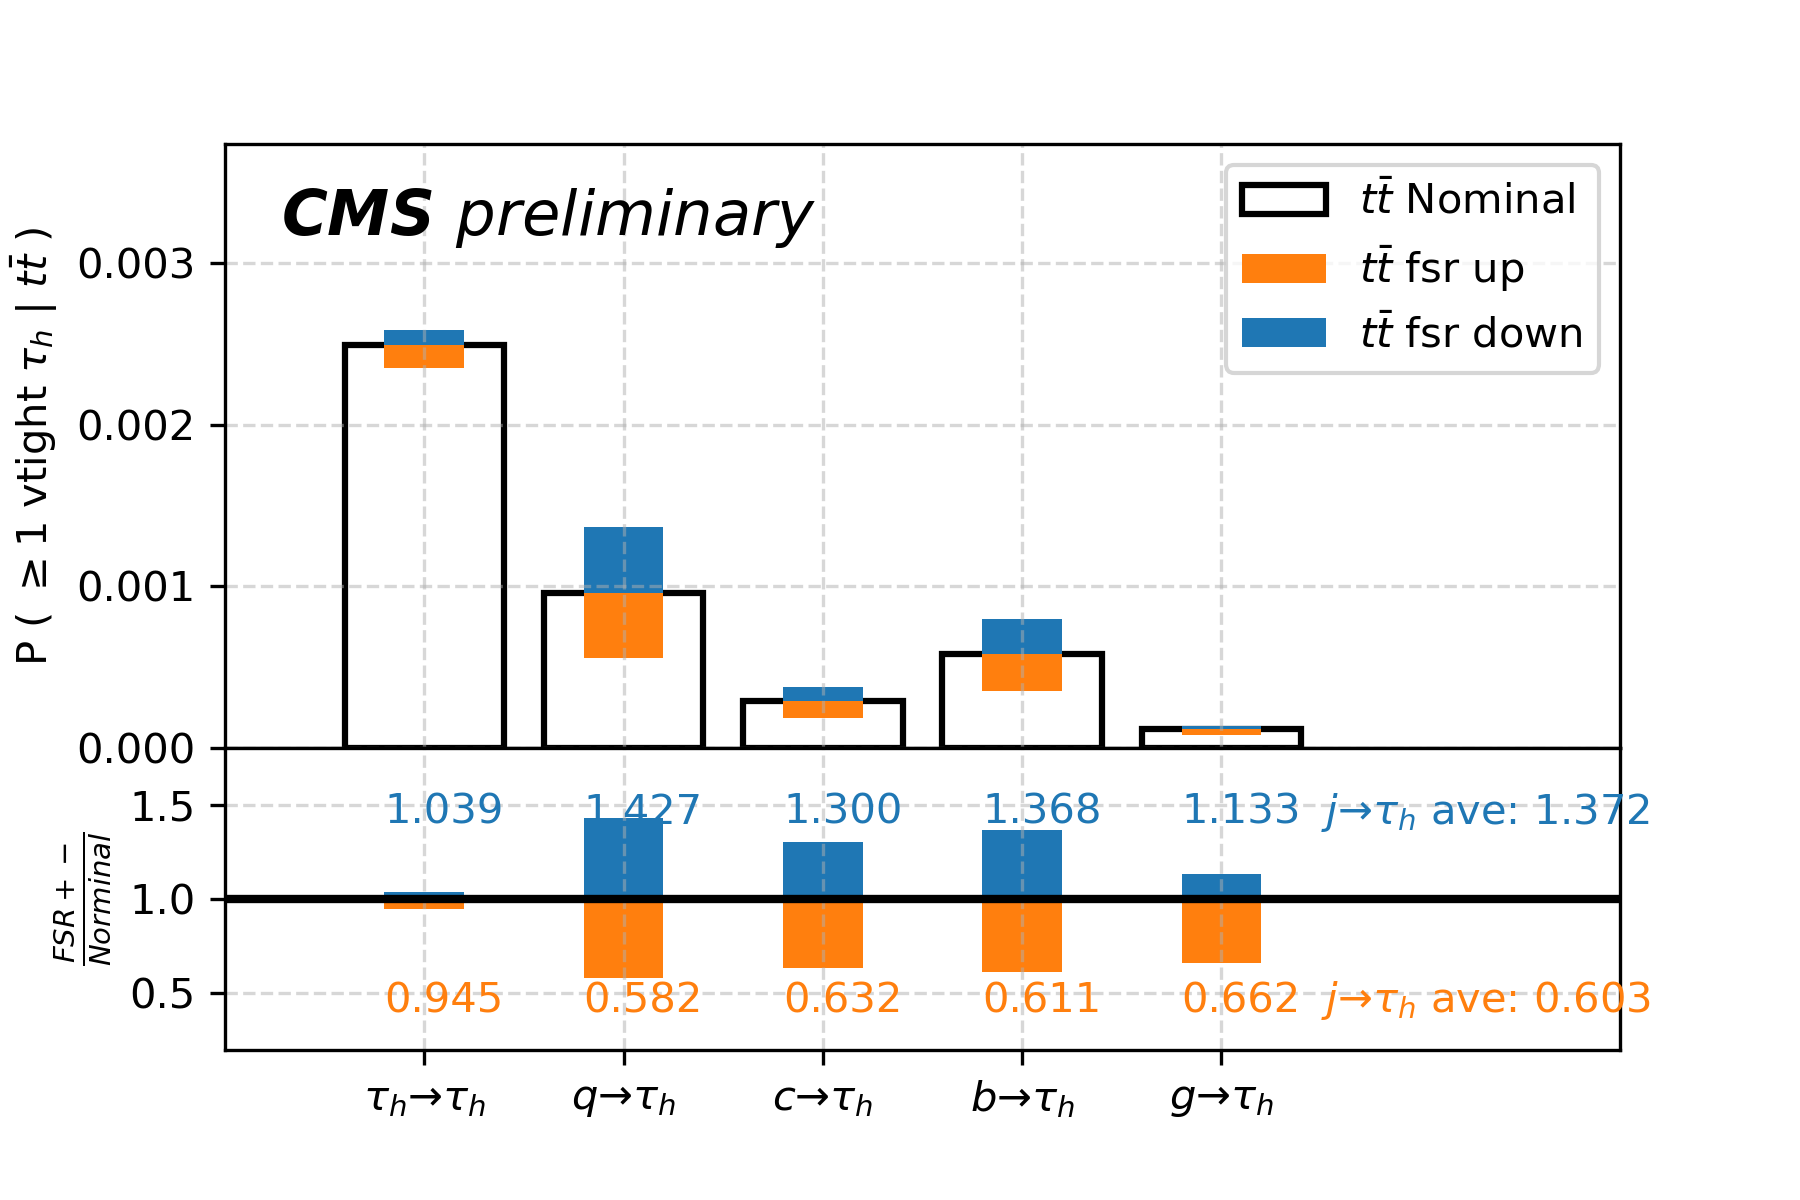
\includegraphics[width=0.49\textwidth]{chapters/Analysis/sectionSystematics/figures/ttTheoretical/2020_MCRatio_fsr_tauGenFlavor_tauVTight.png}
    \end{figure}
\end{frame}



% -------------
% methods
% -------------
\begin{frame}{}%Frame Title}
    \begin{center}
        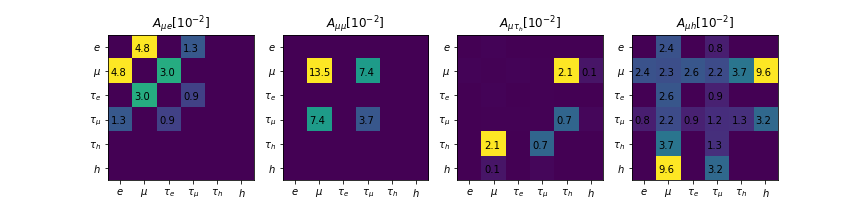
\includegraphics[width=0.7\textwidth]{chapters/Analysis/sectionStatisticalAnalysis/figures/acc_mu1b.png}
        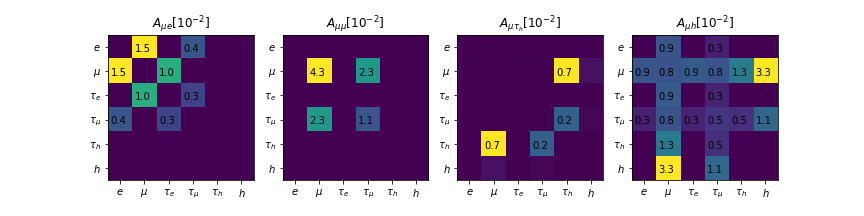
\includegraphics[width=0.7\textwidth]{chapters/Analysis/sectionStatisticalAnalysis/figures/acc_mu2b.png}
        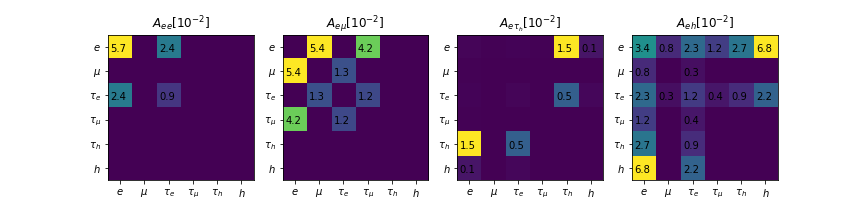
\includegraphics[width=0.7\textwidth]{chapters/Analysis/sectionStatisticalAnalysis/figures/acc_e1b.png}
        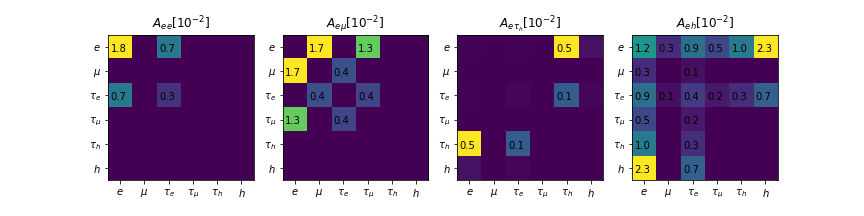
\includegraphics[width=0.7\textwidth]{chapters/Analysis/sectionStatisticalAnalysis/figures/acc_e2b.png}
    \end{center}
\end{frame}



\begin{frame}{Counting combine}
\smaller
    The systematic uncertainties are estimated by the changes of $\{\beta_{e},\beta_{\mu},\beta_{\tau}\}$ when variating up/down the systematical parameters by their $\pm 1\sigma$ uncertainties.
    The four solutions from the four the trigger-$n_b$ regions, $\mu 1b$, $\mu 2b$, $e1b$, $e2b$
    \begin{equation*}
        \tiny
        \beta_0 = \bigg [
        \beta_e^{\mu1b}, \beta_\mu^{\mu1b}, \beta_\tau^{\mu1b}, \quad 
        \beta_e^{\mu2b}, \beta_\mu^{\mu2b}, \beta_\tau^{\mu2b}, \quad 
        \beta_e^{e1b}, \beta_\mu^{e1b}, \beta_\tau^{e1b}, \quad
        \beta_e^{e2b}, \beta_\mu^{e2b}, \beta_\tau^{e2b}
        \bigg ]^T
    \end{equation*}
    
    are combined with a least-chi2 $\chi^2(\beta) = (\beta_0 - \textbf{A} \beta )^T \textbf{V}^{-1} (\beta_0 - \textbf{A} \beta ) $ assuming
    \begin{itemize}
        \item the statistical uncertainties are uncorrelated;
        \item one source of systematic is fully correlated among the four solutions;
        \item different sources of systematics are mutually independent.
    \end{itemize}

    where 
    $\textbf{V} =
    \sum_{n \in \text{data,MC}} \big( \Delta_{n}\beta_0 \big) \otimes   \big( \Delta_{n}\beta_0 \big) +
    \sum_{\theta \in \text{syst}} \big( \Delta_{\theta}\beta_0 \big) \otimes  \big( \Delta_{\theta}\beta_0 \big)
    $
    and $\textbf{A}=[I_{3\times3}, I_{3\times3}, I_{3\times3}, I_{3\times3}]^T$. The combined result $\beta$ can be analytically calculated 
    \begin{equation*}
        \beta =   (\textbf{A}^T \textbf{V}^{-1} \textbf{A})^{-1}(\textbf{A}^T \textbf{V}^{-1}) \beta_0, \quad
        \text{with } \textbf{Var}\big[\beta\big]  =   (\textbf{A}^T \textbf{V}^{-1} \textbf{A})^{-1} .
    \end{equation*}

\end{frame}



\begin{frame}{shape correlation}
    \centering
    \includegraphics[width=0.7\textwidth]{chapters/Analysis/sectionSystematics/figures/correlation_matrix_full.pdf}
\end{frame}



\begin{frame}{}
\centering
counting analysis
    \begin{table}[]
        \setlength{\tabcolsep}{2em}
        \renewcommand{\arraystretch}{1}
        \resizebox{0.99\textwidth}{!}{\begin{table}[]

    
  \renewcommand{\arraystretch}{1.1}
  \setlength{\tabcolsep}{0.4em}
  \centering
  \caption{ Statistical and systematic error of four categories. }
  \resizebox{\textwidth}{!}{
      \begin{tabular}{|l|ccc|ccc|ccc|ccc|ccc|}
      \hline
      Error Source & \multicolumn{3}{c|}{$\mu$-1b} & \multicolumn{3}{c|}{$\mu$-2b} & \multicolumn{3}{c|}{$e$-1b} & \multicolumn{3}{c|}{$e$-2b} \\
      \hline
                    & $B_e$ & $B_\mu$ & $B_\tau$ & $B_e$ & $B_\mu$ & $B_\tau$ & $B_e$ & $B_\mu$ & $B_\tau$ & $B_e$ & $B_\mu$ & $B_\tau$ \\
      \hline
      StatErr of Data                            & 0.543 & 0.533 & 1.243 & 0.714 & 0.637 & 1.492 & 0.743 & 0.557 & 1.520 & 0.904 & 0.707 & 1.807 \\ 
      StatErr of bg MC                           & 0.178 & 0.745 & 0.767 & 0.110 & 0.411 & 0.501 & 0.897 & 0.257 & 1.065 & 0.494 & 0.137 & 0.521 \\ 
      StatErr of sg MC                           & 0.168 & 0.151 & 0.415 & 0.189 & 0.165 & 0.428 & 0.217 & 0.176 & 0.503 & 0.233 & 0.192 & 0.520 \\ 
      \hline
      PDG err of $Br^\tau_e$                     & 0.002 & 0.019 & 0.029 & 0.002 & 0.019 & 0.029 & 0.003 & 0.019 & 0.029 & 0.003 & 0.020 & 0.030 \\ 
      PDG err of $Br^\tau_\mu$                   & 0.047 & 0.017 & 0.098 & 0.047 & 0.017 & 0.099 & 0.041 & 0.013 & 0.101 & 0.043 & 0.013 & 0.106 \\ 
      2.5$\%$ err of luminosity                  & 0.330 & 0.461 & 0.120 & 0.093 & 0.064 & 0.049 & 0.135 & 0.390 & 0.204 & 0.002 & 0.101 & 0.092 \\ 
      5$\%$ err of tt XS                         & 0.002 & 0.000 & 0.151 & 0.009 & 0.015 & 0.032 & 0.021 & 0.011 & 0.148 & 0.011 & 0.002 & 0.003 \\ 
      5$\%$ err of tW XS                         & 0.002 & 0.001 & 0.157 & 0.010 & 0.015 & 0.033 & 0.022 & 0.012 & 0.155 & 0.011 & 0.002 & 0.004 \\ 
      5$\%$ err of t XS                          & 0.062 & 0.062 & 0.033 & 0.053 & 0.052 & 0.058 & 0.063 & 0.060 & 0.032 & 0.052 & 0.054 & 0.040 \\ 
      5$\%$ err of W+Jets XS                     & 0.343 & 0.354 & 0.325 & 0.068 & 0.068 & 0.066 & 0.349 & 0.347 & 0.366 & 0.065 & 0.066 & 0.084 \\ 
      10$\%$ err of Z+Jets XS                    & 0.495 & 2.655 & 0.237 & 0.122 & 0.491 & 0.055 & 1.576 & 0.501 & 0.173 & 0.275 & 0.104 & 0.041 \\ 
      10$\%$ err of $\gamma$+Jets XS             & 0.020 & 0.019 & 0.029 & 0.005 & 0.005 & 0.007 & 0.249 & 0.247 & 0.213 & 0.058 & 0.058 & 0.081 \\ 
      10$\%$ err of VV XS                        & 0.004 & 0.044 & 0.027 & 0.001 & 0.010 & 0.005 & 0.038 & 0.003 & 0.021 & 0.008 & 0.001 & 0.001 \\ 
      25$\%$ err of QCD in $e 4j$                & 0.000 & 0.000 & 0.000 & 0.000 & 0.000 & 0.000 & 1.164 & 1.118 & 2.410 & 0.219 & 0.218 & 0.406 \\ 
      25$\%$ err of QCD in $\mu 4j$              & 0.742 & 0.737 & 1.562 & 0.223 & 0.214 & 0.384 & 0.000 & 0.000 & 0.000 & 0.000 & 0.000 & 0.000 \\ 
      25$\%$ err of QCD in $e\tau$               & 0.000 & 0.000 & 0.000 & 0.000 & 0.000 & 0.000 & 0.372 & 0.498 & 2.651 & 0.069 & 0.092 & 0.503 \\ 
      25$\%$ err of QCD in $\mu\tau$             & 0.345 & 0.465 & 2.360 & 0.185 & 0.250 & 1.285 & 0.000 & 0.000 & 0.000 & 0.000 & 0.000 & 0.000 \\ 
      top pT reweighting                         & 0.000 & 0.000 & 0.032 & 0.002 & 0.003 & 0.007 & 0.004 & 0.002 & 0.031 & 0.002 & 0.000 & 0.001 \\ 
      0.6$\%$ err of $\epsilon_e$ reco           & 0.575 & 0.054 & 0.042 & 0.583 & 0.055 & 0.042 & 0.709 & 0.160 & 0.103 & 0.574 & 0.084 & 0.069 \\ 
      1.4$\%$ err of $\epsilon_e$ id             & 1.386 & 0.129 & 0.101 & 1.410 & 0.133 & 0.101 & 1.766 & 0.335 & 0.275 & 1.456 & 0.163 & 0.197 \\ 
      0.1$\%$ err of $\epsilon_\mu$ reco         & 0.015 & 0.125 & 0.016 & 0.008 & 0.095 & 0.011 & 0.009 & 0.078 & 0.008 & 0.008 & 0.077 & 0.008 \\ 
      0.2$\%$ err of $\epsilon_\mu$ id           & 0.052 & 0.496 & 0.066 & 0.021 & 0.370 & 0.045 & 0.033 & 0.299 & 0.029 & 0.032 & 0.299 & 0.031 \\ 
      5$\%$ err of $\epsilon_\tau$               & 0.745 & 1.004 & 5.091 & 0.694 & 0.937 & 4.823 & 0.723 & 0.967 & 5.146 & 0.700 & 0.937 & 5.111 \\ 
      4.7$\%$ err of $\epsilon_{j\to\tau}$       & 0.460 & 0.620 & 3.145 & 0.307 & 0.414 & 2.129 & 0.458 & 0.613 & 3.260 & 0.290 & 0.388 & 2.115 \\ 
      0.5$\%$ err of $ES_{e}$                    & 0.249 & 0.023 & 0.018 & 0.228 & 0.022 & 0.016 & 0.008 & 0.171 & 0.061 & 0.010 & 0.247 & 0.017 \\ 
      0.2$\%$ err of $ES_{\mu}$                  & 0.095 & 0.092 & 0.033 & 0.093 & 0.092 & 0.035 & 0.013 & 0.116 & 0.011 & 0.012 & 0.114 & 0.012 \\ 
      1.2$\%$ err of $ES_{\tau\to\pi^\pm}$       & 0.034 & 0.046 & 0.232 & 0.035 & 0.047 & 0.244 & 0.034 & 0.046 & 0.245 & 0.030 & 0.040 & 0.216 \\ 
      1.2$\%$ err of $ES_{\tau\to\pi^\pm\pi^0}$  & 0.086 & 0.116 & 0.587 & 0.069 & 0.093 & 0.477 & 0.066 & 0.088 & 0.469 & 0.075 & 0.100 & 0.548 \\ 
      1.2$\%$ err of $ES_{\tau\to3\pi^\pm}$      & 0.026 & 0.035 & 0.175 & 0.026 & 0.034 & 0.177 & 0.024 & 0.032 & 0.172 & 0.024 & 0.032 & 0.176 \\ 
      Single-e Trigger (probe syst)              & 0.218 & 0.020 & 0.016 & 0.222 & 0.021 & 0.016 & 0.029 & 0.032 & 0.004 & 0.036 & 0.004 & 0.009 \\ 
      Single-e Trigger (tag syst)                & 0.495 & 0.046 & 0.036 & 0.503 & 0.047 & 0.036 & 0.063 & 0.088 & 0.080 & 0.037 & 0.013 & 0.038 \\ 
      0.5$\%$ err of $Br_{\tau\to\pi^\pm}$       & 0.008 & 0.011 & 0.047 & 0.009 & 0.012 & 0.050 & 0.008 & 0.011 & 0.047 & 0.009 & 0.012 & 0.055 \\ 
      0.4$\%$ err of $Br_{\tau\to\pi^\pm\pi^0}$  & 0.018 & 0.024 & 0.102 & 0.019 & 0.025 & 0.108 & 0.019 & 0.025 & 0.110 & 0.020 & 0.025 & 0.117 \\ 
      1.1$\%$ err of $Br_{\tau\to\pi^\pm2\pi^0}$ & 0.022 & 0.029 & 0.124 & 0.022 & 0.029 & 0.120 & 0.022 & 0.028 & 0.123 & 0.024 & 0.031 & 0.143 \\ 
      0.5$\%$ err of $Br_{\tau\to3\pi^\pm}$      & 0.015 & 0.021 & 0.094 & 0.017 & 0.022 & 0.102 & 0.016 & 0.021 & 0.100 & 0.017 & 0.022 & 0.106 \\ 
      1.1$\%$ err of $Br_{\tau\to3\pi^\pm\pi^0}$ & 0.009 & 0.011 & 0.043 & 0.010 & 0.012 & 0.046 & 0.009 & 0.011 & 0.043 & 0.010 & 0.012 & 0.046 \\ 
      Pileup                                     & 0.041 & 0.183 & 0.777 & 0.231 & 0.026 & 0.891 & 0.428 & 0.474 & 0.592 & 0.248 & 0.137 & 0.835 \\ 
      JES                                        & 2.300 & 0.750 & 4.421 & 1.823 & 1.543 & 2.968 & 1.681 & 2.370 & 4.577 & 1.681 & 1.773 & 2.993 \\ 
      JER                                        & 0.238 & 0.180 & 0.265 & 0.143 & 0.146 & 0.356 & 0.259 & 0.249 & 0.406 & 0.148 & 0.138 & 0.538 \\ 
      Btag                                       & 0.098 & 0.772 & 0.643 & 0.111 & 0.023 & 0.114 & 0.181 & 0.091 & 0.762 & 0.024 & 0.109 & 0.088 \\ 
      Mistag                                     & 0.100 & 0.141 & 0.035 & 0.100 & 0.056 & 0.090 & 0.077 & 0.142 & 0.124 & 0.030 & 0.096 & 0.135 \\ 
      tt fsr                                     & 0.760 & 0.583 & 0.743 & 0.236 & 0.253 & 0.643 & 0.289 & 0.473 & 0.756 & 1.029 & 0.065 & 1.337 \\ 
      tt isr                                     & 0.724 & 0.747 & 1.105 & 0.720 & 0.723 & 0.876 & 0.317 & 1.060 & 1.414 & 0.043 & 0.830 & 0.062 \\ 
      tt UE                                      & 0.021 & 0.037 & 1.665 & 0.306 & 1.017 & 0.266 & 0.122 & 0.177 & 1.060 & 0.172 & 0.133 & 0.053 \\ 
      tt MEPS                                    & 0.198 & 0.653 & 1.699 & 1.117 & 0.645 & 0.129 & 0.033 & 0.743 & 1.812 & 0.163 & 1.279 & 1.196 \\ 
      \hline
      Total                                      & 3.378 & 3.646 & 8.655 & 3.047 & 2.579 & 6.609 & 3.643 & 3.459 & 9.135 & 2.884 & 2.728 & 6.967 \\ 
      \hline
      \end{tabular}
  }
 
  \label{tab:syst_alt}
\end{table}
}
    \end{table}
\end{frame}


\begin{frame}{Results}
    \begin{center}
        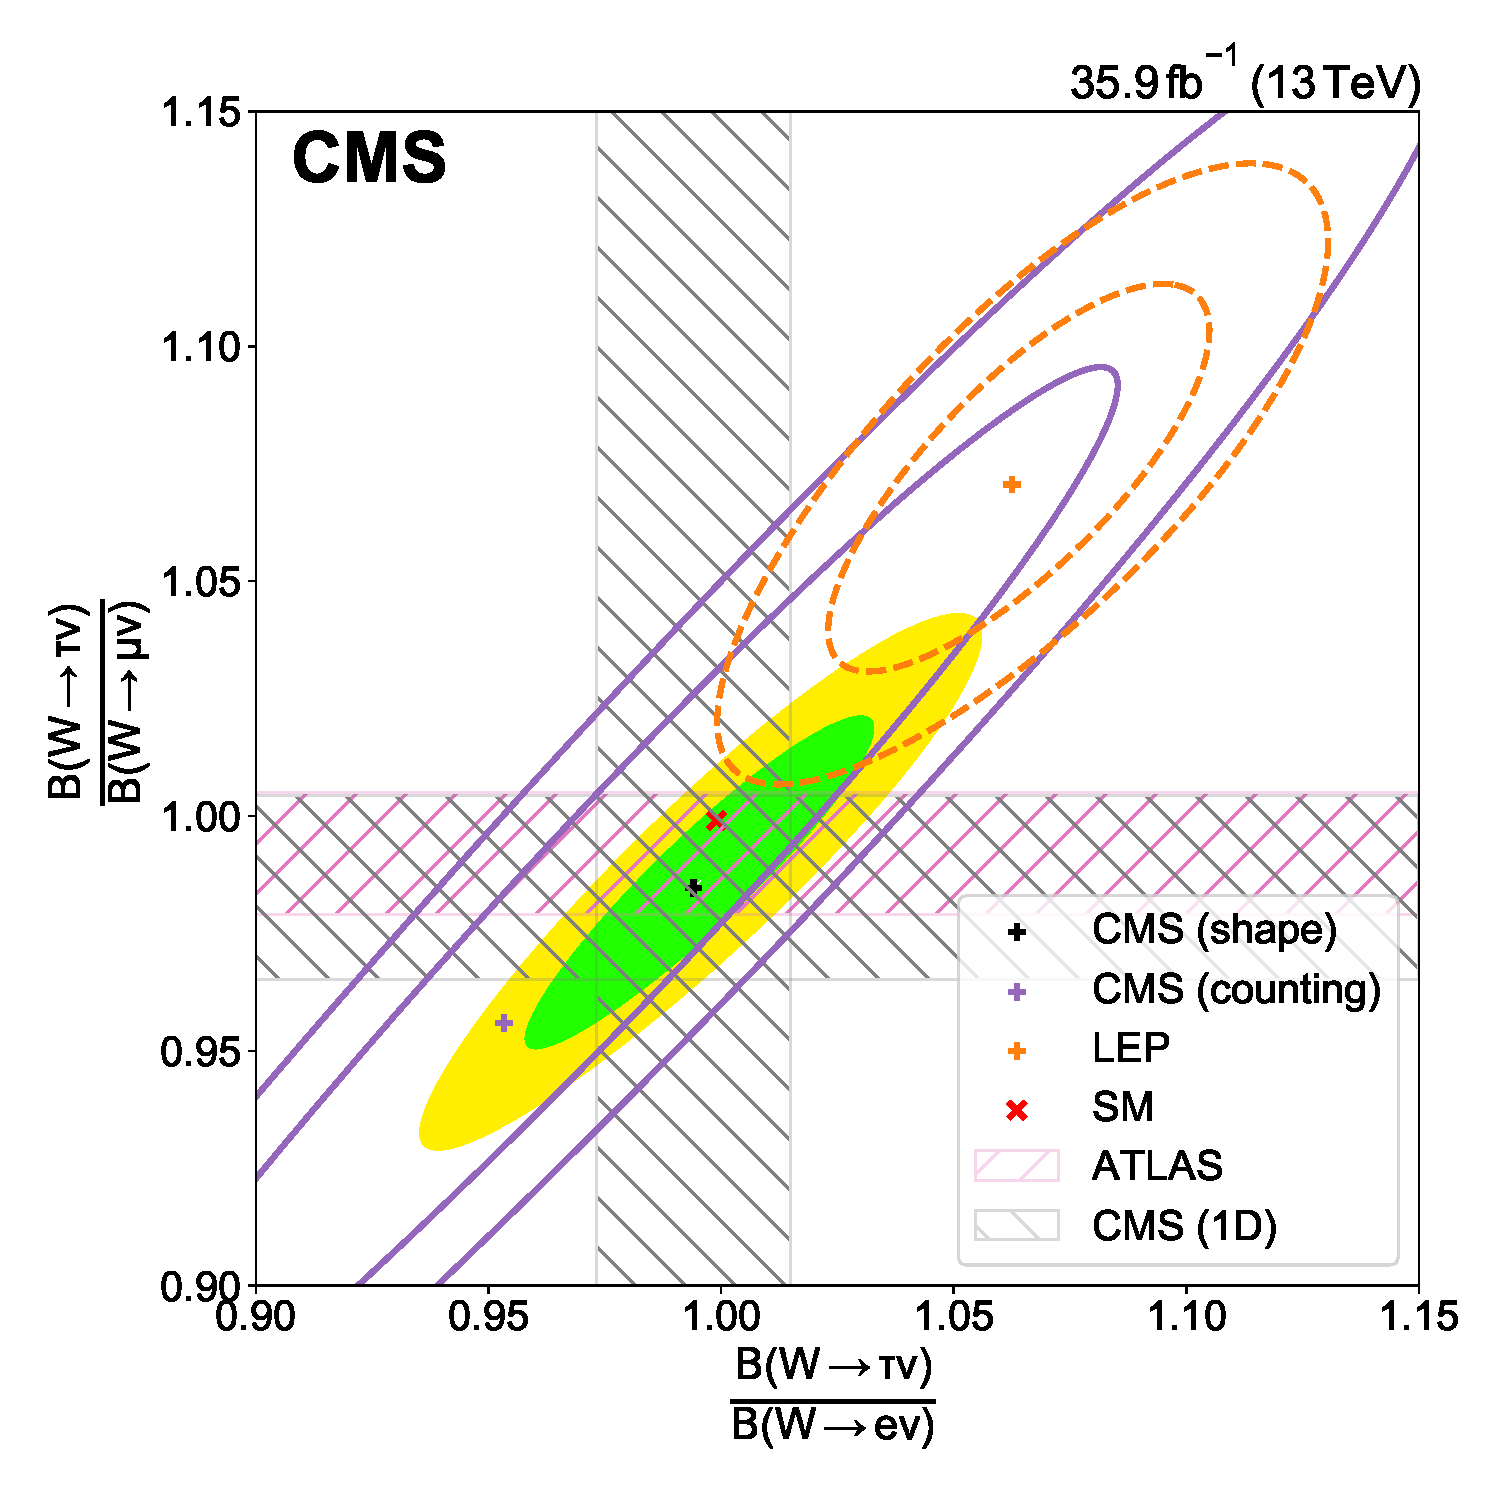
\includegraphics[width=0.6\textwidth]{chapters/Analysis/sectionResult/figures/result_contours_2d_ratio_integral.pdf}
    \end{center}
\end{frame}